\documentclass[11pt,a4paper]{article}

\usepackage[margin=1 in]{geometry}
\usepackage{amsfonts,amsmath,amssymb}
\usepackage[none]{hyphenat}
\usepackage{fancyhdr}
\usepackage{graphicx}
\usepackage{tikz}
\usetikzlibrary{arrows.meta}

% ---------------------------------------------------------------------------
% House diagram style - the same one the probability notes use, so the two
% courses look like they came from the same book. Colours match the accents in
% the web stylesheet; the weight keywords are flattened so no diagram shouts
% next to its neighbour; arrow tips are set once for every picture.
% ---------------------------------------------------------------------------
\definecolor{blue}{HTML}{1D4ED8}
\definecolor{red}{HTML}{B91C1C}
\definecolor{green}{HTML}{12603F}
\definecolor{orange}{HTML}{A16207}
\definecolor{gray}{HTML}{6B7280}

\tikzset{
  every picture/.style={font=\small, line join=round, line cap=round, >=Stealth},
  thin/.style={line width=0.5pt},
  thick/.style={line width=0.9pt},
  very thick/.style={line width=1.1pt},
  ultra thick/.style={line width=1.3pt},
}
\usepackage{color}
\usepackage{xcolor}
\usepackage{array}
\usepackage{float}
\usepackage{multirow}
\usepackage{soul}
\usepackage[nottoc,notlot,notlof]{tocbibind}


% ---------------------------------------------------------------------------
% Tally marks.
%
% These were \StrokeOne .. \StrokeFive from ifsym, which is not installed here
% (it lives in texlive-fonts-extra). Rather than add a dependency that may be
% missing on the next machine, they are drawn with TikZ, which is already
% loaded and which tex4ht converts to SVG for the web.
%
% They matter: the frequency-table sections use them to show how raw
% observations become counts, which is the whole point of the first tally
% column. Dropping them would remove the step being taught.
% ---------------------------------------------------------------------------
\newcommand{\tallystroke}[1]{\draw[line width=.7pt] (#1*0.16,0) -- (#1*0.16,0.32);}
\newcommand{\tallybox}[1]{%
  \raisebox{-0.02em}{\begin{tikzpicture}[baseline=0pt,inner sep=0pt]#1\end{tikzpicture}}%
}
\newcommand{\StrokeOne}  {\tallybox{\tallystroke{0}}}
\newcommand{\StrokeTwo}  {\tallybox{\tallystroke{0}\tallystroke{1}}}
\newcommand{\StrokeThree}{\tallybox{\tallystroke{0}\tallystroke{1}\tallystroke{2}}}
\newcommand{\StrokeFour} {\tallybox{\tallystroke{0}\tallystroke{1}\tallystroke{2}\tallystroke{3}}}
% the fifth stroke crosses the other four, as a tally is actually written
\newcommand{\StrokeFive} {\tallybox{%
  \tallystroke{0}\tallystroke{1}\tallystroke{2}\tallystroke{3}%
  \draw[line width=.7pt] (-0.06,0.04) -- (0.54,0.28);}}



\parindent 0ex

\usetikzlibrary{arrows.meta,shapes,trees,bending,graphs,patterns,quotes,angles}

\pagestyle{fancy}
\fancyhead[R]{}
\renewcommand{\headrulewidth}{0pt}
\fancyfoot[C]{{Page} \thepage}


% ---------------------------------------------------------------------------
% Practice problems, as in the probability notes. These notes define no
% theorem-like environments of their own, so amsthm is loaded here for them.
% build.py collapses each solution into a <details> block on the web, so a
% problem can be attempted before the answer is visible.
% ---------------------------------------------------------------------------
\usepackage{amsthm}
\theoremstyle{definition}
% a plain Definition environment - build.py colours it blue on the web, the
% same as the probability notes
\newtheorem{definition_}{Definition}[section]
\newtheorem{remark_}[definition_]{Remark}
\newtheorem{note_}[definition_]{Note}
\newtheorem{example_}[definition_]{Example}
\newtheorem{problemx}{Problem}[section]
\newenvironment{problem}[1]
  {\begin{problemx}\textup{\small[#1]}\hspace{0.4em}\ignorespaces}
  {\end{problemx}}
\newenvironment{solution}
  {\renewcommand{\qedsymbol}{}\begin{proof}[\textit{Solution}.]}
  {\end{proof}}

% Table rows were padded out with empty '&&&\\' rows to fake vertical
% space. Those render as blank rows on the web; set the spacing properly
% once instead.
\renewcommand{\arraystretch}{1.25}

\begin{document}
% Title page depersonalised for the web: no name, no university, no lecturer,
% no course code. Same treatment as the probability notes - the material is not
% specific to one institution and should not look like an internal handout.
\begin{titlepage}
\begin{center}
\vspace*{4cm}
{\Huge\bfseries Introduction to Statistics}\\[1.2cm]
{\large Lecture Notes}\\[3cm]
\line(1,0){300}
\end{center}
\end{titlepage}

\tableofcontents
\thispagestyle{empty}
\clearpage
\setcounter{page}{1}





\section{Introduction}

\begin{definition_}
\textbf{Statistics} is the science of collecting, organising, analysing and interpreting
data in order to draw conclusions and make decisions in the face of uncertainty.
\end{definition_}

It is convenient to think of the subject in two halves. \textbf{Descriptive statistics} is
concerned with summarising and presenting data that has been collected -- tables, charts,
averages, measures of spread. \textbf{Inferential statistics} goes further, using a sample
to draw conclusions about the larger population it came from, and stating how much
confidence those conclusions deserve.

The whole of this course follows that division: the first chapter is descriptive, and
everything after it is inference.

A statistical investigation ordinarily proceeds through five stages:
\begin{enumerate}
\item \textbf{Collection} -- obtaining the data, by survey, experiment or observation.
\item \textbf{Presentation} -- organising it into tables and charts.
\item \textbf{Analysis} -- computing summaries and fitting models.
\item \textbf{Interpretation} -- deciding what the results actually mean.
\item \textbf{Decision} -- acting on them, which is the point of the exercise.
\end{enumerate}



\begin{definition_}
\textbf{Data} are the recorded values of some characteristic observed on a set of
individuals or items. A single such characteristic is a \textbf{variable}, and each recorded
value is an \textbf{observation}.
\end{definition_}

Data are classified by what can meaningfully be done with the values -- whether they can be
ordered, and whether the gaps between them mean anything. There are four types:
\begin{enumerate}
\item \textbf{Nominal Data}:\\
Used for labelling variables without any quantitative value.\\ Notice that all these labels are mutually exclusive and none of them have numerical significance.
\begin{enumerate}
       \item[$\longrightarrow$] What is your nationality?
       \item[$\longrightarrow$] Where do you live?
\end{enumerate}
\item \textbf{Ordinal Data}\\
With ordinal data it is the order of the values that matters, but the difference between each one is not really known.
\begin{enumerate}
   \item[$\longrightarrow$] How do you feel today?
\end{enumerate}
\item \textbf{Interval Data}\\
Numerical data in which we know not only the order but also the exact difference between the values.
\item \textbf{Ratio Data}\\
These tell us the order and the exact difference between values, and they have a true zero.  There are two types of quantitative data that we are going to study:
\begin{enumerate}
     \item Discrete data
     \item Continuous data\\
\end{enumerate}
\end{enumerate}





In order to develop data analysis skills, it is important to keep the following three points in mind:
\begin{enumerate}
\item For most data sets, there is more than one appropriate and informative way to plot the data.
\item It is valuable to see the same data plotted in several ways, both for the purpose of learning more about data, and because this will help to gain experience in choosing appropriate method of data display and analysis. Professionals routinely do this in order to explore patterns in their data.
\item Creative insights are an asset to good graphing and data analysis. If you invent a different kind of graph that successfully makes a point about the data that can be interpreted by someone else, then the graph is useful.\\
\end{enumerate}















\subsection{Discrete Data}
Discrete data can take only \emph{separate, particular} values, with gaps between them.
Between any two neighbouring values there is nothing a measurement could land on. Such data
usually arise from \textbf{counting}.\\


\textbf{Example}
\begin{enumerate}
\item Marks obtained in a test
\item Number of passengers in  a bus
\item Ages of students in a class.\\
\end{enumerate}



Presentation of discrete data are:
\begin{enumerate}
\item Pie chart
\item Bar chart
\item Pictograph\\
\end{enumerate}

\textbf{Example}
\begin{table}[H]
\begin{tabular}{ccccccccc}
24&42&23&14&20&28&72&13&34\\ 60 &9&4&18&15&13&8&10&51\\
\end{tabular}
\end{table}

The total scores of 30 students out of 5 are given below:
\begin{table}[h!]
\centering
\begin{tabular}{ccccccccccccccc}
3&1&3&2&2&1&1&3&1&1&5&3&3&2&0\\4&2&1&2&5&3&1&2&2&1&1&2&4&2&1\\
\end{tabular}
\end{table}

We can present this type of data in a table called frequency table.\\\\ The difference between the lowest value and highest value is 5


% Table One



\begin{table}[H]
\centering
\begin{tabular}{|c|c|c|}
\hline Score & Tally Mark & $f$ frequency\\
\hline 0& \StrokeOne &1\\
1 & \StrokeFive \StrokeFive & 10\\ 
2 & \StrokeFive \StrokeFour & 9\\
3 & \StrokeFive \StrokeOne  & 6\\
4 & \StrokeTwo              & 2\\ 
5 & \StrokeTwo              & 2\\
\hline
\end{tabular}
\end{table}




\textbf{Bar Chart}


% Diagram 1


\begin{figure}[H]
\centering
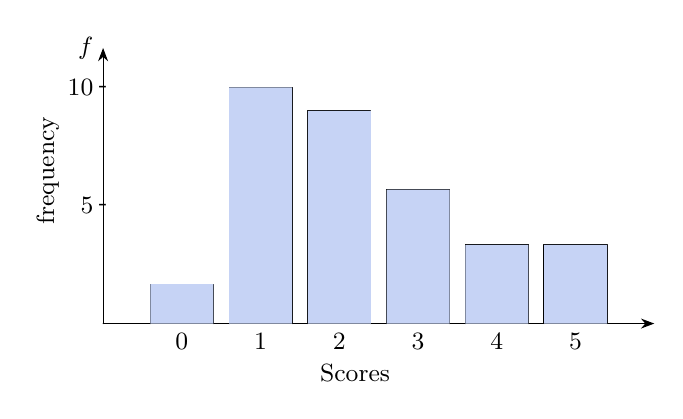
\begin{tikzpicture}
\draw[-Stealth](0,0)--(7,0);
\draw[-Stealth](0,0)--(0,3.5)node[left]{$f$};
\draw(1,0)node[below]{0}
(2,0)node[below]{1}
(3,0)node[below]{2}
(4,0)node[below]{3}
(5,0)node[below]{4}
(6,0)node[below]{5}
(0,1.5)node[left]{5}
(0,3)node[left]{10}
(0,1.5)node[]{-}
(0,3)node[]{-}
(3.2,-0.4)node[below]{Scores};
\draw(0.6,0)--(0.6,0.5)--(1.4,0.5)--(1.4,0)
(1.6,0)--(1.6,3)--(2.4,3)--(2.4,0)
(2.6,0)--(2.6,2.7)--(3.4,2.7)--(3.4,0)
(3.6,0)--(3.6,1.7)--(4.4,1.7)--(4.4,0)
(4.6,0)--(4.6,1)--(5.4,1)--(5.4,0)
(5.6,0)--(5.6,1)--(6.4,1)--(6.4,0);
\path[fill=blue!25]
(0.6,0)--(0.6,0.5)--(1.4,0.5)--(1.4,0)--cycle
(1.6,0)--(1.6,3)--(2.4,3)--(2.4,0)--cycle
(2.6,0)--(2.6,2.7)--(3.4,2.7)--(3.4,0)--cycle
(3.6,0)--(3.6,1.7)--(4.4,1.7)--(4.4,0)--cycle
(4.6,0)--(4.6,1)--(5.4,1)--(5.4,0)--cycle
(5.6,0)--(5.6,1)--(6.4,1)--(6.4,0)--cycle;
\path(-0.7,2)--node[left,sloped]{frequency}(-0.7,3.5);
\end{tikzpicture}
\end{figure}











\subsection{Continuous Data}
Continuous data can take \emph{any} value within a range, with no gaps: between any two
values, however close, another is possible. Such data arise from \textbf{measuring} rather
than counting.

The distinction is about what the quantity \emph{can} be, not how it is written down.
Height recorded to the nearest centimetre is still continuous -- the rounding is a limit of
the ruler, not of the person.\\\\
\textbf{Examples}:
\begin{enumerate}
\item Age
\item Time 
\item Weight
\item Height\\
\end{enumerate}



To present continuous data we also use
\begin{enumerate}
\item Line Plots
\item Histogram
\item Frequency polygon
\item Ogive curve (Cumulative frequency curve)
\item Steam and Leaf plots
\item Two-Way tables
\item Box plots
\item Scatter plots
\item Time-Series plots\\\\
\end{enumerate}



\textbf{Line Plots}
\begin{enumerate}
\item[$\bullet$] Analysis begins by trying to get a good ``picture" of the data.
\item[$\bullet$] A line plot is simply a bar plot (bar graph) where the categories on which we collect data are integers $(0,1,2,3,\cdots,\cdots)$.\\
\end{enumerate}


The method of construction:
\begin{enumerate}
\item[]\textit{Step 1:} Find the smallest and largest values in the data set.
\item[]\textit{Step 2:} Draw a real number line that encompasses these values.
\item[]\textit{Step 3:} Place a mark on the number line corresponding to each data point.\\
\end{enumerate}




\pagebreak
\textbf{Example}\\
A line plot based on  a test:
\begin{figure}[H]
\centering
\begin{tikzpicture}
\draw(0,0)--(9,0)
(1,-0.08)--(1,0.08)
(2,-0.08)--(2,0.08)
(3,-0.08)--(3,0.08)
(4,-0.08)--(4,0.08)
(5,-0.08)--(5,0.08)
(6,-0.08)--(6,0.08)
(7,-0.08)--(7,0.08)
(8,-0.08)--(8,0.08);
\draw(1,-0.08)node[below]{7}
(2,-0.08)node[below]{8}
(3,-0.08)node[below]{9}
(4,-0.08)node[below]{10}
(5,-0.08)node[below]{11}
(6,-0.08)node[below]{12}
(7,-0.08)node[below]{13}
(8,-0.08)node[below]{14};
\draw(2,1)node[below]{*}
(3,1)node[below]{*}
(3,1.5)node[below]{*}
(4,1)node[below]{*}
(4,1.5)node[below]{*}
(4,2)node[below]{*}
(5,1)node[below]{*}
(5,1.5)node[below]{*}
(5,2)node[below]{*}
(5,2.5)node[below]{*}
(5,3)node[below]{*}
(6,1)node[below]{*}
(6,1.5)node[below]{*}
(8,1)node[below]{*}
(8,1.5)node[below]{*}
(8,2)node[below]{*}
(8,2.5)node[below]{*}
(8,3)node[below]{*};
\draw(4.5,-0.7)node[below]{score}
(4.5,3.3)node[above]{class scores on a test};
\end{tikzpicture}
\end{figure}






\vspace{1cm}
\textbf{Frequency, Relative Frequency, and Cumulative Frequency}

\begin{enumerate}
\item[$\bullet$] A frequency is the number of times a given datum occurs in a data set.
\item[$\bullet$] A relative frequency is the fraction of times an answer occurs. To find the relative frequencies, divide each frequency by the total number in the sample.\\
Relative frequencies can be written as fractions, percents, or decimals.

\begin{table}[H]
\centering
\begin{tabular}{|c|c|c|}
\hline
Data Value & Frequency & Relative Frequency\\
\hline
2 & 3 & 3/20\hspace{0.2cm} or\hspace{0.2cm} 0.15\\
3 & 5 & 5/20\hspace{0.2cm} or\hspace{0.2cm} 0.25\\
4 & 3 & 3/20\hspace{0.2cm} or\hspace{0.2cm} 0.15\\
5 & 6 & 6/20\hspace{0.2cm} or\hspace{0.2cm} 0.30\\
6 & 2 & 2/20\hspace{0.2cm} or\hspace{0.2cm} 0.10\\
7 & 1 & 1/20\hspace{0.2cm} or\hspace{0.2cm} 0.05\\
\hline
\end{tabular}
\end{table}

\item[$\bullet$] The sum of the relative frequency column is 20/20, or 1.
\item[$\bullet$] Cumulative relative frequency is the accumulation of the previous relative frequencies.
\begin{table}[H]
\centering
\begin{tabular}{|c|c|c|c|}
\hline
           &           &                    &  Cumulative Relative\\
Data Value & Frequency & Relative Frequency &  Frequency\\           
\hline
2 & 3 & 3/20\hspace{0.2cm} or\hspace{0.2cm} 0.15 & 0.15\\
3 & 5 & 5/20\hspace{0.2cm} or\hspace{0.2cm} 0.25 & 0.15 + 0.25=0.40\\
4 & 3 & 3/20\hspace{0.2cm} or\hspace{0.2cm} 0.15 & 0.40 + 0.15=0.55\\
5 & 6 & 6/20\hspace{0.2cm} or\hspace{0.2cm} 0.30 & 0.55 + 0.30=0.85\\
6 & 2 & 2/20\hspace{0.2cm} or\hspace{0.2cm} 0.10 & 0.85 + 0.10=0.95\\
7 & 1 & 1/20\hspace{0.2cm} or\hspace{0.2cm} 0.05 & 0.95 + 0.05=1.00\\
\hline
\end{tabular}
\end{table}
\end{enumerate}





\textbf{Note:}\\
Because of rounding, the relative frequency column may not always sum to one and the last entry in the cumulative relative frequency column may not be one. However, they each should be close to one.\\\\






We can arrange data into groups or take them as individual values.\\\\
If we consider 5 values, say 3, 5, 0, 2, 6.\\
In grouping data, we can either take individual values or arrange then in intervals called class interval.



% Table 2


\begin{table}[H]
\centering
\begin{tabular}{|c|c|c|}
\hline Value & Tally Marks & $f$\\
\hline 0 & \StrokeFive & 5\\
1 & \StrokeTwo   & 2\\
2 & \StrokeOne   & 1\\ 
3 & \StrokeThree & 3\\
\hline
\end{tabular}
\end{table}




To determine class interval, find the range and divide by 10
% Table 3







\begin{table}[H]
\centering
\begin{tabular}{|c|c|c|c|}
\hline Class & Tally & $f$ & True Class\\
Interval & Marks && Limits\\
\hline 
$1-5$   & \StrokeOne   & 1 & $0.5-5.5$\\
$6-10$  & \StrokeTwo   & 2 & $5.5-10.5$\\
$11-15$ & \StrokeThree & 3 & $10.5-15.5$\\
$16-20$ & \StrokeOne   & 1 & $15.5-20.5$\\
$21-25$ & \StrokeTwo   & 2 & $20.5-25.5$\\
$26-30$ & \StrokeOne   & 1 &$25.5-30.5$\\
 \hline
\end{tabular}
\end{table}





\vspace{0.6cm}

\textbf{Choice Of Class Interval}\\
It is important that the class interval in chosen so that the graph gives a clear representation of the Data. Choice of too large a class interval will lead to loss of details on the other hand too small a class  interval would destroy the originality of the Data. A Convenient rule of thumb is to choose a class  interval so that the Average frequency is about 5.\hspace{0.2cm}\\ i.e. Number of classes = $\dfrac{1}{5}\times$ Total frequency.


\begin{table}[H]
\centering
\caption{Frequency Table}
\label{table: Freguency Table}
\begin{tabular}{|c|c|c|c|}
\hline Class & $f$ & Cumulative & Middle Point\\
Interval && frequency & of the interval\\
\hline $4.0-6$&1&1&5\\
$6.0-8$&3&4&7\\
$8.0-10$&7&11&9\\
$10.0-12$&9&20&11\\
$12.0-14$ &9&29&13\\
$14.0-16$ &12&41&15\\
$16.0-18$&8&49&17\\
$18.0-20$&1&50&19\\
\hline
\end{tabular}
\end{table}


Construct a Histogram using the given table:\\\\





% Diagram 2

\begin{figure}[H]
\centering
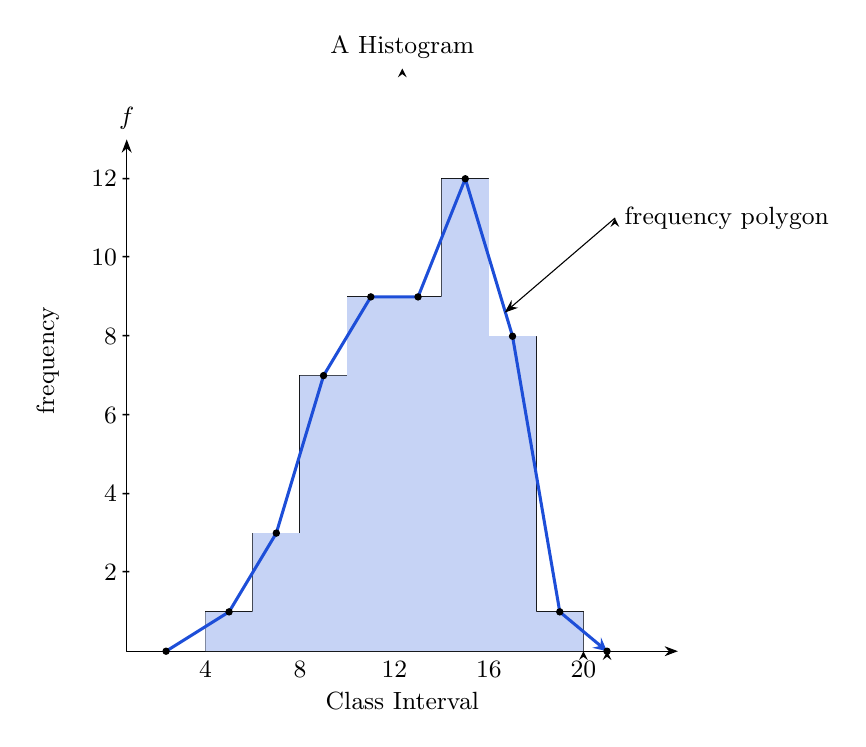
\begin{tikzpicture}[->,>=stealth]
\draw[-Stealth](1,0)--(8,0);
\draw[-Stealth](1,0)--(1,6.5)node[above]{$f$};
\draw(2,0)--(2,0.5)--(2.6,0.5)--(2.6,0)--cycle
(2.6,0)--(2.6,1.5)--(3.2,1.5)--(3.2,0)--cycle
(3.2,0)--(3.2,3.5)--(3.8,3.5)--(3.8,0)--cycle
(3.8,0)--(3.8,4.5)--(4.4,4.5)--(4.4,0)--cycle
(4.4,0)--(4.4,4.5)--(5,4.5)--(5,0)--cycle
(5,0)--(5,6)--(5.6,6)--(5.6,0)--cycle
(5.6,0)--(5.6,4)--(6.2,4)--(6.2,0)--cycle
(6.2,0)--(6.2,0.5)--(6.8,0.5)--(6.8,0)--cycle;
\path[fill=blue!25]
(2,0)--(2,0.5)--(2.6,0.5)--(2.6,0)--cycle
(2.6,0)--(2.6,1.5)--(3.2,1.5)--(3.2,0)--cycle
(3.2,0)--(3.2,3.5)--(3.8,3.5)--(3.8,0)--cycle
(3.8,0)--(3.8,4.5)--(4.4,4.5)--(4.4,0)--cycle
(4.4,0)--(4.4,4.5)--(5,4.5)--(5,0)--cycle
(5,0)--(5,6)--(5.6,6)--(5.6,0)--cycle
(5.6,0)--(5.6,4)--(6.2,4)--(6.2,0)--cycle
(6.2,0)--(6.2,0.5)--(6.8,0.5)--(6.8,0)--cycle;
\draw[very thick,blue](1.5,0)--(2.3,0.5)--(2.9,1.5)--(3.5,3.5)--(4.1,4.5)--(4.7,4.5)--(5.3,6)--(5.9,4)--(6.5,0.5)--(7.1,0);
\draw(1.5,0)node[shape=circle,scale=0.01cm,fill=black]{}
(2.3,0.5)node[shape=circle,scale=0.01cm,fill=black]{}
(2.9,1.5)node[shape=circle,scale=0.01cm,fill=black]{}
(3.5,3.5)node[shape=circle,scale=0.01cm,fill=black]{}
(4.1,4.5)node[shape=circle,scale=0.01cm,fill=black]{}
(4.7,4.5)node[shape=circle,scale=0.01cm,fill=black]{}
(5.3,6)node[shape=circle,scale=0.01cm,fill=black]{}
(5.9,4)node[shape=circle,scale=0.01cm,fill=black]{}
(6.5,0.5)node[shape=circle,scale=0.01cm,fill=black]{}
(7.1,0)node[shape=circle,scale=0.01cm,fill=black]{};
\draw(1,1)node[]{-}
(1,1)node[left]{2}
(1,2)node[left]{4}
(1,2)node[]{-}
(1,3)node[]{-}
(1,3)node[left]{6}
(1,4)node[]{-}
(1,4)node[left]{8}
(1,5)node[]{-}
(1,5)node[left]{10}
(1,6)node[]{-}
(1,6)node[left]{12}
(2,0)node[below]{4}
%(2.6,0)node[below]{6}
(3.2,0)node[below]{8}
%(3.8,0)node[below]{10}
(4.4,0)node[below]{12}
%(5,0)node[below]{14}
(5.6,0)node[below]{16}
%(6.2,0)node[below]{18}
(6.8,0)node[below]{20};
%(7.4,0)node[below]{22};
\draw(4.5,-0.4)node[below]{Class Interval}
(4.5,7.4)node[above]{A Histogram};
\path(0,3)--node[sloped,left]{frequency}(0,6);
\draw[-Stealth](7.2,5.5)--(5.8,4.3);
\draw(7.2,5.5)node[right]{frequency polygon};
\end{tikzpicture}
\end{figure}

\vspace{1cm}













% Diagram 3

\begin{figure}[H]
\centering
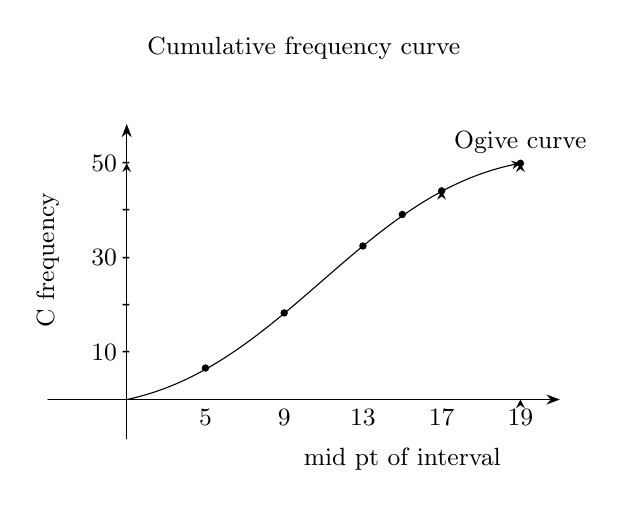
\begin{tikzpicture}[->,>=stealth]
\draw[-Stealth](-1,0)--(5.5,0);
\draw[-Stealth](0,-0.5)--(0,3.5);
\draw(0,0)..controls(2,0.42)and(3,2.64)..(5,3);
\draw(1,0)node[below]{5}
(2,0)node[below]{9}
(3,0)node[below]{13}
(4,0)node[below]{17}
(5,0)node[below]{19};
\draw(0,0.6)node[]{-}
(0,1.2)node[]{-}
(0,1.8)node[]{-}
(0,2.4)node[]{-}
(0,3)node[]{-}
(0,0.6)node[left]{10}
(0,1.8)node[left]{30}
(0,3)node[left]{50};
\draw(2,1.1)node[shape=circle,scale=0.01cm,fill=black]{}
(3.5,2.35)node[shape=circle,scale=0.01cm,fill=black]{}
(3,1.95)node[shape=circle,scale=0.01cm,fill=black]{}
(5,3)node[shape=circle,scale=0.01cm,fill=black]{}
(1,0.4)node[shape=circle,scale=0.01cm,fill=black]{}
(4,2.65)node[shape=circle,scale=0.01cm,fill=black]{};
\draw(2.25,4.2)node[above]{Cumulative frequency curve}
(3.5,-0.5)node[below]{mid pt of interval}
(5,3)node[above]{Ogive curve};
\path(-1,2.5)--node[left,sloped]{C frequency}(-1,3);
\end{tikzpicture}
\end{figure}

















\subsection{Histogram With Unequal Class Intervals}
Grouped frequency table are sometimes given with unequal class intervals because a particular range of the variate may be of special interest.\\ If you do this, care has to be exercised in calculating the true class limits as age in the table below is measured differently from other variates. e.g. $18-20$ includes people who are just 18 to those one day less than 21.\\ Since the eyes compares area and not height in a histogram the areas of the blocks must be proportional to class frequency\\\\
$\therefore$ height of block $\alpha$ $\dfrac{\text{class frequency}}{\text{class width}}$\\\\

The ratio $\dfrac{\text{class frequency}}{\text{class width}}$ is known as the frequency density.\\\\

\begin{table}[H]
\centering
\begin{tabular}{|c|c|c|c|c|c|}
\hline Class & True Class & Class & frequency & frequency & Relative\\
Interval & Limit & Width & $(.000)$ & Density & Frequency\\
\hline $16-17$ & $16-18$ & 2& 4&2 & $8.316\times 10^{-1}$\\
$18-20$ & $18-21$ &3 &73&24.33&0.1518\\
$21-24$ & $21-25$ & 4 & 185& 46.25&0.3846\\
$25-29$&$25-30$&5&104&20.8&0.2162\\
$30-34$&$30-35$&5&34&6.8&0.0707\\
$35-44$&$35-44$&10&33&3.3&0.0686\\
$45-54$&$45-55$&10&22&2.2&0.0457\\
55 and above & 55 and above &20&26&1.3&0.0540\\
$55-75$&$55-75$&&&&\\
\hline
\end{tabular}
\end{table}

Construct a (1) Histogram (2) Ogive curve\\\\\\









\textbf{Stem-and-Leaf Plots}\\
A stem-and-leaf plot provides an alternative to a line plot or histogram for obtaining a picture of the data distribution when data can be represented as integer (counting) numbers.

\begin{figure}[H]
\centering
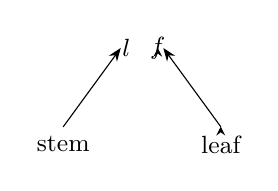
\begin{tikzpicture}[->,>=stealth]
\draw(-0.2,0)node[]{$l$}
(0.2,0)node[]{$f$};
\draw[-Stealth](-1,-1)--(-0.27,0);
\draw[-Stealth](1,-1)--(0.27,0);
\draw(-1,-1)node[below]{stem}
(1,-1)node[below]{leaf};
\end{tikzpicture}
\end{figure}




The method of construction:\\
$\bullet$ Find the largest and smaller scores. They are best explained in the context of an example.\\


\textbf{Example}\\
Make a stem and leaf plot of the algebra test scores given below.
\begin{table}[H]
\centering
\begin{tabular}{ccccccccc}
56 & 65 & 98 & 82 & 64 & 71 & 78 & 77 & 86\\
69 & 70 & 80 & 92 & 76 & 82 & 85 & 91 & 92\\
95 & 99 & 91 & 73 & 59
\end{tabular}
\end{table}



\begin{enumerate}
\item[$\bullet$] Since the data ranges from 56 to 96, the stems range from 5 to 9.
\item[$\bullet$] To plot the data, make a vertical list of the stems.
\item[$\bullet$] Each number is assigned to the graph by pairing the units digit, or leaf, with the correct stem.
\item[$\bullet$] The score 56 is plotted by placing the units digit, 6, to the right of stem 5.
\end{enumerate}


\begin{table}[H]
\centering
\begin{tabular}{c|ccccccc}
Stem & \multicolumn{7}{l}{Leaf}\\
\hline
5 & 6 & 9 &   &  &  & & \\
6 & 4 & 5 & 9 &  &  & & \\
7 & 0 & 1 & 3 & 6 & 7 & 8 & \\
8 & 0 & 2 & 2 & 5 & 6 & & \\
9 & 1 & 1 & 2 & 2 & 5 & 8 & 9\\
\end{tabular}
\end{table}





\begin{enumerate}
\item[$\bullet$] The stem-and-leaf represents a histogram when turned vertically.
\item[$\bullet$] The lowest score on the algebra test is 56.
\item[$\bullet$] The highest score on the algebra test is 99.
\item[$\bullet$] The interval in which most students scored is 90 to 99.\\
\end{enumerate}




Data with more than two digits can be rounded to two digits before plotting or can be truncated to two digits. For a stem and leaf plot, you would truncate everything after the second digit.
\begin{enumerate}
\item[$\bullet$] The number 355 would round to 36.
\item[$\bullet$] The number 355 would truncate to 35.\\\\\\
\end{enumerate}





\textbf{Box Plots}
\begin{enumerate}
\item[$\bullet$] Provides a visual representation of a five-number summary of data, consisting of the median (the midpoint of the data range), the upper and lower quartiles (the numbers below the highest quarter of the data and above the lowest quarter, respectively) and largest and smallest values (the extremes).
\item[$\bullet$] Box plots are particularly useful for comparing distributions of the results from several experimental conditions.\\
\end{enumerate}



``Because box plots are based on simple summaries, they can be used with fairly young children certainly third graders"\\\\




Constructing the graph:
\begin{enumerate}
\item[\textit{Step 1:}] Determine the five-number summary (lower extreme, lower quartile, median,upper quartile and upper extreme).
\item[\textit{Step 2:}] Construct a number line that includes the extremes.
\item[\textit{Step 3:}] Mark the position of the five numbers in the summary a little above the number line.
\item[\textit{Step 4:}] Draw a narrow box that connects the quartiles. Draw a line through the box at the median. Draw lines from the ends of the boxes to the extremes (``Whiskers").\\
\end{enumerate}






\textbf{Example}
\begin{table}[H]
\begin{tabular}{ccccccccc}
\multicolumn{9}{c}{sit-up/min}\\
49 & 58 & 57 & 43 & 46 & 35 & 42 & 56 & 50\\
47 & 45 & 45 & 43 & 51 & 36 & 41 & 50 & 48\\
\end{tabular}
\end{table}





The five number summary. Written in the order of the lower extreme, lower quartile, median, upper quartile, and upper extreme is:
\begin{table}[H]
\centering
\begin{tabular}{ccccc}
34 & 41 & 45.5 & 50 64
\end{tabular}
\end{table}





A box plot of these numbers, plotted above the real number line for reference, would look like the following:


\begin{figure}[H]
\centering
\begin{tikzpicture}
\draw(0,0)--(10,0)
(1,-0.08)--(1,0.08)
(2,-0.08)--(2,0.08)
(3,-0.08)--(3,0.08)
(4,-0.08)--(4,0.08)
(5,-0.08)--(5,0.08)
(6,-0.08)--(6,0.08)
(7,-0.08)--(7,0.08)
(8,-0.08)--(8,0.08)
(9,-0.08)--(9,0.08);
\draw(1,-0.08)node[below]{30}
(3,-0.08)node[below]{40}
(5,-0.08)node[below]{50}
(7,-0.08)node[below]{60}
(9,-0.08)node[below]{70}
(5,-0.5)node[below]{sit-up/min};
\draw(7.9,1)node[shape=circle,scale=0.01cm,fill=black,thick]{}
(5,1)node[shape=circle,scale=0.01cm,fill=black,thick]{}
(4.1,1)node[shape=circle,scale=0.01cm,fill=black,thick]{}
(3.2,1)node[shape=circle,scale=0.01cm,fill=black,thick]{}
(1.8,1)node[shape=circle,scale=0.01cm,fill=black,thick]{};
\draw(7.9,1)--(5,1)
(5,0.7)--(5,1.3)
(4.1,0.7)--(4.1,1.3)
(3.2,0.7)--(3.2,1.3)
(1.8,1)--(3.2,1)
(3.2,0.7)--(5,0.7)
(3.2,1.3)--(5,1.3);
\end{tikzpicture}
\end{figure}









\vspace{0.7cm}




\subsection{Data Collection}
Our interest in this course is quantitative data. Before anything can be done with it, one
question has to be settled: where did it come from? Data are either gathered by the
investigator, or taken from someone who gathered it earlier.

\begin{definition_}[Primary data]
\textbf{Primary data} are collected first-hand, by the investigator, for the specific
purpose at hand.
\end{definition_}

The usual methods are:
\begin{enumerate}
\item \textbf{Questionnaires} -- reach many respondents cheaply, but only the questions
asked get answered, and a badly worded one cannot be repaired afterwards.
\item \textbf{Oral or personal interview} -- allows a vague answer to be followed up, at
the cost of time and of the interviewer's own influence on the reply.
\item \textbf{Observation} -- recording what people do rather than what they say they do,
which avoids the gap between the two.
\item \textbf{Experiment} -- the investigator sets the conditions rather than waiting to
see what occurs, and this is the only method that can establish cause.
\end{enumerate}

\begin{definition_}[Secondary data]
\textbf{Secondary data} were collected by somebody else, for some other purpose, and are
being reused here.
\end{definition_}

Common sources are newspapers, journals, government and agency reports, and published
statistical abstracts.

\begin{remark_}
The trade-off between them is worth stating plainly, because it decides which to use.

Primary data are collected to answer \emph{your} question, so they measure what you want,
on the population you care about, in the form you need. They are expensive and slow.

Secondary data are immediate and often free, and may be far larger than anything you could
gather yourself. But they were defined by someone else's purpose: the categories may not be
the ones you want, the population may not be quite yours, the collection may be out of date,
and you cannot ask how carefully it was done. Whenever secondary data are used, the source
should be recorded along with the figures.
\end{remark_}





\pagebreak

\subsection{Measures Of Central Tendencies}
Central tendency: of a distribution is an estimate of the "center" of a distribution of values.\\ There are three major types of estimates of central tendency
\begin{enumerate}
\item Mean
\item Median
\item Mode\\\\
\end{enumerate}






\begin{enumerate}
\item \textbf{Mean}\\
The mean is probably the most commonly used method of describing central tendency.\\\\ 
\textbf{Definition}\\
The mean is the central value of the given observation.
\begin{align*}
&\textbf{Notation}\\
\sum \hspace{0.3cm}&-\hspace{0.3cm}\text{Sum}\\\
\overline{X}\hspace{0.3cm}&-\hspace{0.3cm}\text{Mean}\\
n\hspace{0.3cm}&-\hspace{0.3cm}\text{Number of observations}
\end{align*}



$$\overline{X}=\frac{1}{n}\sum_1^nX\hspace{1cm}\text{Ungrouped Data}$$
The mean is determined by summing all the observations and dividing by the number of observations.\\




\begin{example_}
Find the mean of the values $0,\ 5,\ 2,\ 3,\ 5$.
\end{example_}

\begin{solution}
$$\overline{X}=\frac{1}{n}\sum_{i=1}^{5}X_i=\frac{0+5+2+3+5}{5}=\frac{15}{5}=3.$$
\end{solution}

For data already summarised in a frequency table, each value is weighted by how often it
occurs:
$$\overline{X}=\frac{\sum fX}{\sum f}.$$

\begin{example_}
Find the mean of the data below.
\begin{table}[H]
\centering
\begin{tabular}{lcccc}
$X$ & 0 & 1 & 2 & 3\\
\hline
$f$ & 3 & 2 & 2 & 1\\
\end{tabular}
\end{table}
\end{example_}

\begin{solution}
Add an $fX$ row and total both:
\begin{table}[H]
\centering
\begin{tabular}{lccccr}
$X$  & 0 & 1 & 2 & 3 & Total\\
\hline
$f$  & 3 & 2 & 2 & 1 & 8\\
$fX$ & 0 & 2 & 4 & 3 & 9\\
\end{tabular}
\end{table}
$$\overline{X}=\frac{\sum fX}{\sum f}=\frac{9}{8}=1.125.$$
\end{solution}

When the data have been grouped into classes the individual values are no longer available,
so each observation is represented by the \textbf{mid-point} of its class.

\begin{example_}
Estimate the mean of the grouped data below.
\begin{table}[H]
\centering
\begin{tabular}{lcccc}
Class interval & $1$--$5$ & $6$--$10$ & $11$--$15$ & $16$--$20$\\
\hline
$f$ & 1 & 3 & 2 & 1\\
\end{tabular}
\end{table}
\end{example_}

\begin{solution}
The mid-point of a class is the average of its two limits: for $1$--$5$ that is
$(1+5)/2=3$, and so on.
\begin{table}[H]
\centering
\begin{tabular}{lrrr}
Class interval & Mid-point $X$ & $f$ & $fX$\\
\hline
$1$--$5$   & 3  & 1 & 3\\
$6$--$10$  & 8  & 3 & 24\\
$11$--$15$ & 13 & 2 & 26\\
$16$--$20$ & 18 & 1 & 18\\
\hline
Total      &    & 7 & 71\\
\end{tabular}
\end{table}
$$\overline{X}=\frac{\sum fX}{\sum f}=\frac{71}{7}=10.14.$$
\end{solution}

\begin{example_}
Calculate the mean for each of the following sets of data.
\begin{enumerate}
\item[(a).] The raw values $15,\ 20,\ 21,\ 20,\ 36,\ 15,\ 25,\ 15$.
\item[(b).] Data summarised in a frequency table:
\begin{table}[H]
\centering
\begin{tabular}{lcccccc}
$X$ & 0 & 1 & 2 & 3 & 4 & 5\\
\hline
$f$ & 3 & 5 & 3 & 2 & 1 & 1\\
\end{tabular}
\end{table}
\item[(c).] Data grouped into classes:
\begin{table}[H]
\centering
\begin{tabular}{lccccccc}
Class interval & $1$--$5$ & $6$--$10$ & $11$--$15$ & $16$--$20$ & $21$--$25$ & $26$--$30$ & $31$--$35$\\
\hline
$f$ & 1 & 3 & 5 & 4 & 2 & 2 & 1\\
\end{tabular}
\end{table}
\end{enumerate}
\end{example_}

\begin{solution}
The three parts are the same calculation at three levels of summary, and each level costs
a little accuracy.

\textbf{(a). Raw values.} Every observation is present, so the mean is exact:
$$\overline{X}=\frac{1}{n}\sum X=\frac{15+20+21+20+36+15+25+15}{8}=\frac{167}{8}=20.875.$$

\textbf{(b). Frequency table.} The individual values are still known; they have only been
counted rather than listed. Multiply each value by how often it occurs:
\begin{table}[H]
\centering
\begin{tabular}{lccccccr}
$X$    & 0 & 1 & 2 & 3 & 4 & 5 & Total\\
\hline
$f$    & 3 & 5 & 3 & 2 & 1 & 1 & 15\\
$fX$   & 0 & 5 & 6 & 6 & 4 & 5 & 26\\
\end{tabular}
\end{table}
$$\overline{X}=\frac{\sum fX}{\sum f}=\frac{26}{15}=1.733.$$
This is still exact -- writing $2$ three times or writing ``$2$, three times'' is the same
information.

\textbf{(c). Grouped data.} Here the individual values are \emph{gone}. All we know is how
many fell in each class, so each observation is taken to sit at its class mid-point:
\begin{table}[H]
\centering
\begin{tabular}{lrrr}
Class interval & Mid-point $X$ & $f$ & $fX$\\
\hline
$1$--$5$   & 3  & 1  & 3\\
$6$--$10$  & 8  & 3  & 24\\
$11$--$15$ & 13 & 5  & 65\\
$16$--$20$ & 18 & 4  & 72\\
$21$--$25$ & 23 & 2  & 46\\
$26$--$30$ & 28 & 2  & 56\\
$31$--$35$ & 33 & 1  & 33\\
\hline
Total      &    & 18 & 299\\
\end{tabular}
\end{table}
$$\overline{X}=\frac{\sum fX}{\sum f}=\frac{299}{18}=16.61.$$

This last answer is an \textbf{estimate}, not the mean of the original data. Treating every
observation in $11$--$15$ as though it were exactly $13$ is only right on average, and the
error does not necessarily cancel. Once data have been grouped, the exact mean cannot be
recovered -- which is worth remembering before grouping data you still need to work with.
\end{solution}






\item \textbf{Median and Interquartile Range}\\

The median is the value found on the middle  of the set of the ordered observations.\\ 
One way to compute the median is to list all scores in numerical order, and locate the score on the middles of the observation.\\ When you order the observations $n$ can either be odd or even
\begin{enumerate}
    \item if $n$ is odd, then the median is one of the observations.
    \item if $n$ is even, the median is not one of the observation.\\
\end{enumerate}


\textbf{Example}\\
Find the medians
\begin{enumerate}
\item 15, 20, 21, 20, 36, 15, 25, 15\\

\begin{table}[H]
\centering
(b) $\hspace{1cm}$
\begin{tabular}{|c|c|}
\hline $X$ & $f$\\
\hline 0&3\\
1&5\\ 2&3\\ 3&2\\ 4&1\\ 5&1\\
\hline
\end{tabular}
$\hspace{2cm}$
(c) $\hspace{1cm}$
\begin{tabular}{|c|c|}
\hline
Class Interval & $f$\\
\hline $1-5$&1\\
$6-10$&3\\
$11-15$&5\\
$16-20$&4\\
$21-25$&2\\
$26-30$&2\\
$31-35$&1\\
\hline
\end{tabular}
\end{table}
\end{enumerate}


\textbf{Solution}
\begin{enumerate}
\item 15, 15, 20, 20, 21, 25, 36
$$\therefore\hspace{1cm} \text{Median}=\frac{20+20}{2}=20$$\\

\begin{table}[H]
\centering
(b)$\hspace{1cm}$
\begin{tabular}{|c|c|c|}
\hline $X$ & $f$ & $Cf$\\
\hline 0&3&3\\
1&5&8\\
2&3&11\\
3&2&13\\
4&1&14\\
5&1&15\\
\hline
\end{tabular}
$\hspace{1cm}$ $n=1\hspace{0.5cm}\implies$ Md = 8$^{\text{th}}$ value = 1\\
\end{table}
\end{enumerate}
\vspace{0.4cm}


\textbf{median from a frequency table for discrete data}\\
If data is not grouped the median can easily be found by arranging the data in order.\\ In the table below we can use the Cf to find the median.\\

\begin{table}[H]
\centering
\begin{tabular}{|c|c|c|}
\hline Score & $f$ & Cf\\
\hline 1&7&7\\
2&15&22\\ 3&10&32\\ 4&3&35\\ 5&9&44\\ 6&6&50\\
\hline
\end{tabular}
\end{table}


$n=50\hspace{0.5cm}\implies$ Md = 25$^{\text{th}}$ value and 26$^{\text{th}}$ value = $\dfrac{3+3}{2}=3$.\\\\

\textbf{Median of a Continuous Data}\\
\begin{table}[H]
\centering
\begin{tabular}{|c|c|c|c|}
\hline C.I & $f$ & Cf & True Upper Class Limits\\
\hline $4.0-5.9$ & 1 & 1 & 5.95\\
$6.0-7.9$ & 3 & 4 & 7.95\\
$8.0-9.9$ & 7 & 11 & 9.95\\
$10.0-11.9$ & 9 & 20 & 11.95\\
$12.0-13.9$ & 9 & 29 & 13.95\\
$14.0-15.9$ & 12 & 41 & 15.95\\
$16.0-17.9$ & 8 & 49 & 17.95\\
$18.0-19.9$ &1 & 50 & 19.95\\
\hline
\end{tabular}
\end{table}

If we assume the curve is linear between $A$ and $B$.\\\\


% Diagram 6

\begin{figure}[H]
\centering
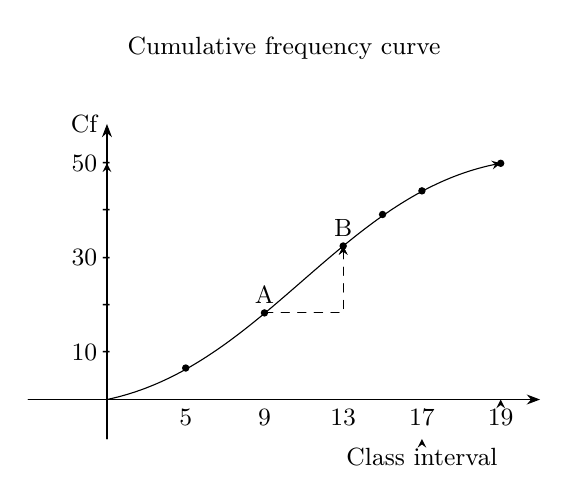
\begin{tikzpicture}[->,>=stealth]
\draw[-Stealth](-1,0)--(5.5,0);
\draw[-Stealth](0,-0.5)--(0,3.5)node[left]{Cf};
\draw(0,0)..controls(2,0.42)and(3,2.64)..(5,3);
\draw(1,0)node[below]{5}
(2,0)node[below]{9}
(3,0)node[below]{13}
(4,0)node[below]{17}
(5,0)node[below]{19};
\draw(0,0.6)node[]{-}
(0,1.2)node[]{-}
(0,1.8)node[]{-}
(0,2.4)node[]{-}
(0,3)node[]{-}
(0,0.6)node[left]{10}
%(0,1.2)node[left]{20}
(0,1.8)node[left]{30}
%(0,2.4)node[left]{40}
(0,3)node[left]{50};
\draw(2,1.1)node[shape=circle,scale=0.01cm,fill=black]{}
(3.5,2.35)node[shape=circle,scale=0.01cm,fill=black]{}
(3,1.95)node[shape=circle,scale=0.01cm,fill=black]{}
(5,3)node[shape=circle,scale=0.01cm,fill=black]{}
(1,0.4)node[shape=circle,scale=0.01cm,fill=black]{}
(4,2.65)node[shape=circle,scale=0.01cm,fill=black]{}
(2,1.1)node[above]{A}
(3,1.95)node[above]{B};
\draw[dashed](2,1.1)--(3,1.1)--(3,1.95);
\draw(2.25,4.2)node[above]{Cumulative frequency curve}
(4,-0.5)node[below]{Class interval};
\end{tikzpicture}
\end{figure}


$\dfrac{50}{2}=25^{\text{th}}$ value and $26^{\text{th}}$ value.













% DIAGRAM 7

\begin{figure}[H]
\centering
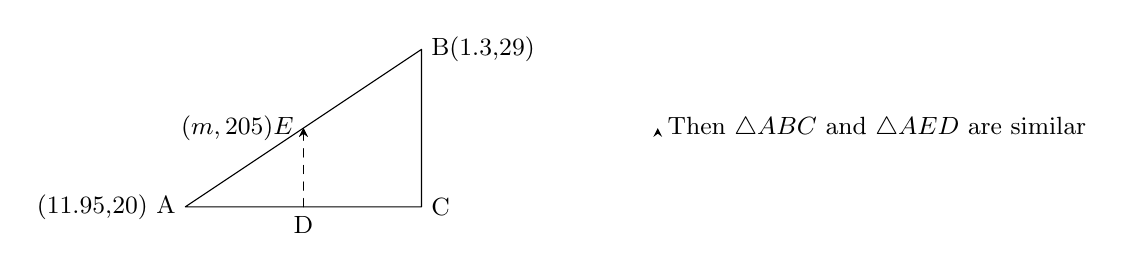
\begin{tikzpicture}[->,>=stealth]
\draw(0,0)--(3,0)--(3,2)--cycle;
\draw[dashed](1.5,0)--(1.5,1);
\draw(0,0)node[left]{(11.95,20) A}
(1.5,0)node[below]{D}
(3,0)node[right]{C}
(3,2)node[right]{B(1.3,29)}
(1.5,1)node[left]{$(m,205)E$};
\draw(6,1)node[right]{Then $\triangle ABC$ and $\triangle AED$ are similar};
\end{tikzpicture}
\end{figure}
$\dfrac{AD}{AC}=\dfrac{ED}{BC}\hspace{1cm}\implies \hspace{0.5cm} m=13.06$\\\\



Median Grouped Data
\begin{enumerate}
\item[\textit{Step 1:}] Construct the cumulative frequency distribution.
\item[\textit{Step 2:}] Decide the class that contain the median. \textit{Class Median} is the first class with the value of cumulative frequency equal at least $n/2$.
\item[\textit{Step 3:}] Find the median by using the following formula:
   $$\text{Median} = L_m + \Bigg(\dfrac{\dfrac{n}{2}-F}{f_m}\Bigg)\, i$$
\end{enumerate}



Where:
\begin{enumerate}
\item[]$n = $ the total frequency
\item[]$F = $ the cumulative frequency before class median
\item[]$f_m = $ the frequency of the class median
\item[]$i = $ the class width
\item[]$L_m = $ the lower boundary of the class median\\
\end{enumerate}




\textbf{Example}\\
Based on the grouped data below, find the median
\begin{table}[H]
\centering
\begin{tabular}{|c|c|}
\hline
Time to travel & \\
to work        & Frequency\\
\hline
$1 - 10$ & 8\\
$11 - 20$ & 14\\
$21 - 30$ & 12\\
$31 - 40$ & 9\\
$41 - 50$ & 7\\
\hline
\end{tabular}
\end{table}
\vspace{0.5cm}





\textbf{Solution:}\\
\textit{Step 1:} Construct the cumulative frequency distribution.


\begin{table}[H]
\centering
\begin{tabular}{|c|c|c|}
\hline
Time to travel &  & Cumulative\\
to work        & Frequency & Frequency\\
\hline
$1 - 10$ & 8    & 8\\
$11 - 20$ & 14  & 22\\
$21 - 30$ & 12  & 34\\
$31 - 40$ & 9   & 43\\
$41 - 50$ & 7   & 50\\
\hline
\end{tabular}
\end{table}

$\displaystyle{\frac{n}{2}=\frac{50}{2}=25}\implies$ Class median is the $3^{\text{rd}}$ class.\\

So\hspace{0.2cm} $F=22,\hspace{0.2cm} f_m=12,\hspace{0.2cm} L_m=21.5\hspace{0.2cm}$ and $\hspace{0.2cm}i=10$.\hspace{0.2cm} Therefore

\begin{align*}
\text{Median} & = L_m + \Bigg(\dfrac{\dfrac{n}{2}-F}{f_m}\Bigg)\, i\\\\
              & = 21.5 + \Bigg(\dfrac{25-22}{12}\Bigg)\times 10\\
              & = 24
\end{align*}
Thus, 25 persons take less than 24 minutes to travel to work and another 25 persons take more than 24 minutes to travel to work.\\\\




\textbf{Quartiles}\\
Using the same method of calculation as in the median. We can get $Q_1$ and $Q_3$ equation as follows:
$$Q_1 = L_{Q_1} + \Bigg(\dfrac{\dfrac{n}{4}- F}{f_{Q_1}}\Bigg) \, i$$

$$Q_3 = L_{Q_3} + \Bigg(\dfrac{\dfrac{3n}{4}- F}{f_{Q_3}}\Bigg) \, i$$\\




\textbf{Example}\\
Based on the grouped data below, find the interquartile range.
\begin{table}[H]
\centering
\begin{tabular}{|c|c|}
\hline
Time to travel & \\
to work        & Frequency\\
\hline
$1 - 10$ & 8\\
$11 - 20$ & 14\\
$21 - 30$ & 12\\
$31 - 40$ & 9\\
$41 - 50$ & 7\\
\hline
\end{tabular}
\end{table}
\vspace{0.5cm}





\textbf{Solution:}\\
\textit{Step 1:} Construct the cumulative frequency distribution.


\begin{table}[H]
\centering
\begin{tabular}{|c|c|c|}
\hline
Time to travel &  & Cumulative\\
to work        & Frequency & Frequency\\
\hline
$1 - 10$ & 8    & 8\\
$11 - 20$ & 14  & 22\\
$21 - 30$ & 12  & 34\\
$31 - 40$ & 9   & 43\\
$41 - 50$ & 7   & 50\\
\hline
\end{tabular}
\end{table}


\textit{Step 2:} Determine the $Q_1$ and $Q_3$\\

Class $\displaystyle{Q_1 = \dfrac{n}{4} = \dfrac{50}{4}=12.5}\implies$ Class $Q_1$ is the $2^{\text{nd}}$ class.  Therefore,
\begin{align*}
Q_1 & = L_{Q_1} + \Bigg(\dfrac{\dfrac{n}{4}-F}{f_{Q_1}}\Bigg)\, i\\\\
    & = 10.5 + \Bigg(\dfrac{12.5-8}{14}\Bigg)\times 10\\\\
\implies Q_1 & = 13.7143\\
\end{align*}



Class $Q_3  = \displaystyle{\dfrac{3n}{4} = \dfrac{3(50)}{4} = 37.5} \implies$ Class $Q_3$ is the $4^{\text{th}}$ class. Therefore,
\begin{align*}
Q_3 & = L_{Q_3} + \Bigg(\dfrac{\dfrac{3n}{4}-F}{f_{Q_3}}\Bigg)\, i\\\\
    & = 30.5 + \Bigg(\dfrac{37.5-34}{9}\Bigg)\times 10\\\\
\implies Q_3 & = 34.3889\\
\end{align*}


Interquartile Range: \hspace{0.2cm} $IQR = Q_3 - Q_1$\\

Calculate the $IQR$
\begin{align*}
IQR & = Q_3 - Q_1\\
    & = 34.3889 - 13.7143\\
    & = 20.6746\\
\end{align*}












\item \textbf{Mode}\\
The mode is the most frequently occurring value in the data set.\\ If the data is not grouped the mode is simply the value that appears most. But if data is grouped in C.I we call this as mode class.\\


\textbf{Example}\\
Find the mode of the following
\begin{enumerate}
  \item 1, 2, 3, 4, 5 $\implies$ Mode = no mode.
  \item 0, 1, 4, 0, 3, 0, 1, 7, 1, 9 $\implies$ Mode is 0 $\&$ 1
 
 
\begin{table}[H]
\centering
\text{(c)}$\hspace{3cm}$
\begin{tabular}{c|c}
$X$ & $f$\\
\hline 0&7\\
1&2\\ 2&1\\ 3&4\\
\end{tabular}
$\hspace{1cm}\implies\hspace{0.3cm}$
Mode = 0\\
\end{table}

\begin{table}[H]
\centering
\text{(d).}$\hspace{3cm}$
\begin{tabular}{c|c}
C.I & $f$\\
\hline
$1-5$&1\\
$6-10$&3\\
$11-15$&3\\
$16-20$&3\\
\end{tabular}
$\hspace{1cm}\implies\hspace{0.3cm}$ Mode = $6-10$ and $11-15$.\\
\end{table}
\end{enumerate}

\vspace{0.5cm}




Mode-Grouped Data
\begin{enumerate}
\item[$\bullet$] For grouped data, class mode (or modal class) is the class with the highest frequency.
\item[$\bullet$] To find mode for grouped data, use the following formula: $$\text{Mode} = L_{m_o} + \Bigg(\dfrac{\Delta1}{\Delta1 + \Delta_2}\Bigg)\, i$$

where:
\begin{enumerate}
\item[$i$] is the class width
\item[$\Delta_1$] is the difference between the frequency of class mode and the frequency of the class after the class mode.
\item[$\Delta_2$] is the difference between the frequency of class mode and frequency of the class before the class mode.
\item[$L_{m_0}$] is the lower boundary of class mode.\\\\
\end{enumerate}




\textbf{Example}\\
Based on the grouped data below, find the mode.
\begin{table}[H]
\centering
\begin{tabular}{|c|c|}
\hline
Time to travel & \\
to work        & Frequency\\
\hline
$1 - 10$ & 8\\
$11 - 20$ & 14\\
$21 - 30$ & 12\\
$31 - 40$ & 9\\
$41 - 50$ & 7\\
\hline
\end{tabular}
\end{table}

\vspace{0.5cm}
\textbf{Solution}\\
Based on the table\hspace{0.3cm} $L_{m_0} = 10.5\hspace{0.1cm},\hspace{0.2cm} \Delta_1 = (14-8)=6\hspace{0.1cm},\hspace{0.2cm}\Delta_2 = (14-12)=2\hspace{0.2cm}$ and $\hspace{0.2cm} i = 10$

\begin{align*}
\text{Mode}  & = 10.5 + \Bigg(\dfrac{6}{6 + 2}\Bigg)\times 10\\
& = 17.5\\
\end{align*}
\end{enumerate}














Selecting among the mode, median and mean. The choice of the measure of central tendency depends on the distribution of the data at hand.\\ If the data at hand is assumed to normally distributed $N\thicksim (0,1)$ mean will give a true reflection of the data, otherwise we consider the mode or median.\\\\
\end{enumerate}

The first consideration is the type of data. If the variable is categorical, the mode is the single measure that best describe the data.\\ The second consideration in selecting the index is to ask whether the total of all observation is of any interest, if the answer is yes, then the mean is the proper index of the central tendency. If the total is of no interest then depending on whether the histogram is symmetric on skewed one must use either mean or median respectively.\\ In all cases the histogram must be unimodal.\\

\subsection{Measure Of Dispersion}
The mean itself is not of good indication of quality of data. You need to know the variance to make an educated assessment.\\ Statistical measures are often used for describing the nature and extend of differences among the information in the distribution.\\ A measure of variability is generally reported together with measure of central tendency.\\ Statistical measures of variation are numerical values that indicate the variability inherent in a set of data measurements.\\ Quality of data is measured by its variability.\\ If the variability is large indicates low quality of data.\\ If the variability is small, the that measures the values are cluster about the mean-good.\\\\ The four common measures of variation are: Range, Variance, Standard deviation and Coefficient of variation.\\

\subsection{Range}
The range is simply the highest value minus the lowest value.\\ The range is not a good indicator of the distribution of the observation since it considers two values only, The highest and the lowest.\\



\textbf{Example}\\
Find the range of the following distribution

\begin{table}[H]
\centering
\begin{tabular}{ccccccccccc}
20,&23,&30,&33,&21,&19,&28,&36,&32,&25,&29\\\\\\
\end{tabular}
\end{table}



\subsection{Standard Deviation}
The standard deviation is a more accurate and detailed estimate of dispersion because an out lies can greatly exaggerate the range.\\ The standard deviation shows the relation that set of scores has to the mean of the sample.\

\begin{align*}
& \textbf{Notation}\\
\sum &- \text{Summation}\\
\sigma^2 &- \text{Variance}\\
\sigma &- \text{Standard Deviation}\\
X &- \text{Variable}\\
\overline{X} &- \text{Mean}\\
n &- \text{Number of observations}\\
\end{align*}

We can calculate the standard deviation from either ungrouped data or grouped data.\\



\begin{enumerate}
\item \textbf{Ungrouped Data}\\
The formula used to calculate s.d. for ungrouped data is $$\sigma =\sqrt{\frac{\sum (X-\overline{X})^2}{n}}$$\\
\textbf{Example}\\ 
Calculate $\sigma$ for the following values: 0, 1, 3, 5, 6\\\\



\textbf{Solution}\\

$\displaystyle{\overline{X}=\frac{0+1+3+5+6}{5}=\frac{15}{5}=3\hspace{1cm}\implies\hspace{0.5cm} \overline{X}=3}$\\

\begin{table}[H]
\centering
\begin{tabular}{|c|c|c|}
\hline Value & $X-\overline{X}$ & $(X-\overline{X})^2$\\
\hline 0& $-3$ &9\\
1 & $-2$ & 4\\ 3&0&0\\ 5&2&4\\ 6&3&9\\
\hline &0&26\\
\hline
\end{tabular}
\end{table}

\begin{align*}
\sigma^2 &=\frac{\sum (X-\overline{X})^2}{n}=\frac{26}{5}\\\\
\implies\hspace{0.5cm} \sigma &=\pm \sqrt{\frac{26}{5}}\\\\
\implies\hspace{0.5cm}\sigma & =2.28035085\hspace{1cm} \implies\hspace{0.5cm} \sigma \approx 2.28\\
\end{align*}

\item Calculation of $\sigma$ from grouped data $$\sigma=\sqrt{\frac{\sum (X-\overline{X})^2}{\sum f}}$$\\







\begin{table}[H]
\centering
\begin{tabular}{|c|c|c|c|c|c|}
\hline $X$& $f$ & $f(X)$&$X-\overline{X}$& $(X-\overline{X})^2$&$f(X-\overline{X})^2$\\
\hline 0&3&0&$-1.1$&1.21&3.63\\
1&4&4&$-0.1$&0.01&0.04\\
2&2&4&0.9&0.81&1.62\\
3&1&3&1.9&3.61&3.61\\
\hline &10&11&&&8.90\\
\hline
\end{tabular}
\end{table}

$$\sigma=\sqrt{\frac{\sum f(X-\overline{X})}{\sum f}}=\sqrt{\frac{8.90}{10}}=0.94\hspace{1cm} \implies\hspace{0.5cm} \sigma =0.94$$\\





\textbf{Example}\\
Calculate the standard deviation for the following the set of values
\begin{table}[H]
\centering
\begin{tabular}{|c|c|}
\hline C.I & $f$\\
\hline $4-6$ & 1\\
$7-9$& 3\\
$10-12$ & 5\\
$13-15$&2\\
$16-18$&1\\
\hline
\end{tabular}
\end{table}
\end{enumerate}




\vspace{0.5cm}

\subsection{Mean Deviation}
This is a measure of dispersion which uses the values of the variance. It is found by finding the deviation of each value of the variate from the mean and find the absolute value of the deviation and then find the mean of those deviations.\\
$$\text{M.D}=\frac{\sum |X-\overline{X}|}{n}\hspace{0.5cm}\text{for ungrouped data}$$\\
$$\text{M.D} = \frac{\sum f|X-\overline{X}|}{\sum f}\hspace{0.5cm}\text{for grouped data}$$\\

\textbf{Examples}\\
Find the mean deviation of the following:
\begin{enumerate}
\item 1, 2, 3, 4, 5, 6, 7\\

\begin{table}[H]
\centering
2. $\hspace{1cm}$
\begin{tabular}{c|c}
$X$ & $f$\\
\hline 1& 4\\
2&6\\
3&12\\
4&6\\
5&6\\
6&1\\
\end{tabular}
$\hspace{3cm}$
3.$\hspace{1cm}$
\begin{tabular}{c|c}
C-I & $f$\\
\hline $1-5$&1\\
$6-10$ & 3\\
$11-15$& 4\\
$16-20$&2\\
\end{tabular}
\end{table}
\end{enumerate}







\vspace{0.2cm}
\subsection{Quartiles}

Quartiles involves dividing the given ordered data into four equal points


% Draw Q



\begin{figure}[H]
\centering
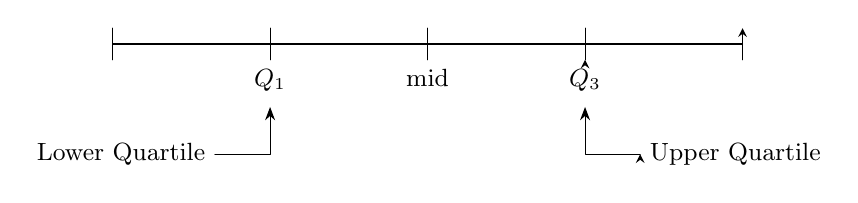
\begin{tikzpicture}[->,>=stealth]
\draw(-4,0)--(4,0)
(-4,-0.2)--(-4,0.2)
(-2,-0.2)--(-2,0.2)
(0,-0.2)--(0,0.2)
(2,-0.2)--(2,0.2)
(4,-0.2)--(4,0.2);
\draw(-2,-0.2)node[below]{$Q_1$}
(0,-0.2)node[below]{mid}
(2,-0.2)node[below]{$Q_3$};
\draw[-Stealth](-2.7,-1.4)--(-2,-1.4)--(-2,-0.8);
\draw[-Stealth](2.7,-1.4)--(2,-1.4)--(2,-0.8);
\draw(-2.7,-1.4)node[left]{Lower Quartile}
(2.7,-1.4)node[right]{Upper Quartile};
\end{tikzpicture}
\end{figure}








\vspace{0.3cm}
\textbf{Interquartile Range}\\
This is a measure of dispersion which extends the ideal of the median. The median divides the data into two equal parts. If we, now find the middle value of each half, we have for the lower half $Q_1=$ lower quartile and the upper half, we have the upper quartile $=Q_3$. These divide the distribution into quartiles.$$\text{Interquartile Range}\hspace{0.3cm}=Q_3-Q_1$$ $$\text{Semi Interquartile Range}\hspace{0.3cm}=\frac{1}{2}(Q_3-Q_1)$$\\
We can see that the quartiles are $\dfrac{1}{4}(n+1)^{\text{th}}$ value and $\dfrac{3}{4}(n+1)^{\text{th}}$ values.\\\\

\textbf{Example}\\
 Find the interquartile range\\

\begin{table}[H]

\begin{tabular}{c|cccccccccc}
$X$&1&2&3&4&5&6&7&8&9&10\\
\hline
$f$&2&8&9&5&4&3&4&1&1&1\\
\end{tabular}
\end{table}
\vspace{0.3cm}


\textbf{Interquartile Range for grouped data}\\
For the data grouped into class interval we can estimate the quartiles from cumulative frequency curve


% Diagram 8

\begin{figure}[H]
\centering
\begin{tikzpicture}[->,>=stealth]
\draw[-Stealth](-1,0)--(4.5,0);
\draw[-Stealth](0,-1)--(0,3.5);
\draw(0,0)..controls(1.5,0.42)and(2,2.64)..(4,3);
\draw[-Stealth,dashed](0,0.75)--(1.14,0.75)--(1.14,0);
\draw[-Stealth,dashed](0,2.25)--(2.5,2.25)--(2.5,0);
\draw(1.14,0)node[below]{$Q_1$}
(2.5,0)node[below]{$Q_3$}
(0,2.25)node[left]{$\frac{3}{4}(n+1)^{\text{th}} Q_3$}
(0,0.75)node[left]{$\frac{1}{4}(n+1)^{\text{th}} Q_1$};
\end{tikzpicture}
\end{figure}








If $\sum f=10$\\\\
$Q_1$ is the $\dfrac{11}{4}^{\text{th}}$ observation $\dfrac{11}{4}=2.75\implies Q_1$ lies between the 2$^{\text{nd}}$ value and the $3^{\text{nd}}$ value.\\\\
$Q_3$ is the $\dfrac{3}{4}\times 11^{\text{th}}$ observation $\dfrac{3}{4}\times 11=\frac{33}{4}=8.25\implies Q_3$ lies between $8^{\text{th}}$ value and $9^{\text{th}}$ value.\\\\

\subsection{Percentiles}

This means we divide the ordered  data into 100 equal parts.

% P


\begin{figure}[H]
\centering
\begin{tikzpicture}[->,>=stealth]
\draw(-4,2)--(4,2)
(-4,1.8)--(-4,2.2)
(-2,1.8)--(-2,2.2)
(0,1.8)--(0,2.2)
(2,1.8)--(2,2.2)
(4,1.8)--(4,2.2);
\draw(-2,1.8)node[below]{$P_{25}$}
(0,1.8)node[below]{$P_{50}$}
(2,1.8)node[below]{$P_{75}$}
(-4.5,2)node[left]{Percentiles};
\draw(-4,0)--(4,0)
(-4,-0.2)--(-4,0.2)
(-2,-0.2)--(-2,0.2)
(0,-0.2)--(0,0.2)
(2,-0.2)--(2,0.2)
(4,-0.2)--(4,0.2);
\draw(-2,-0.2)node[below]{$Q_1$}
(0,-0.2)node[below]{mid}
(2,-0.2)node[below]{$Q_3$}
(-4.5,0)node[left]{Quartiles};
\draw(-4,-2)--(4,-2)
(-4,-1.8)--(-4,-2.2)
(-2,-1.8)--(-2,-2.2)
(0,-1.8)--(0,-2.2)
(2,-1.8)--(2,-2.2)
(4,-1.8)--(4,-2.2);
\draw(-2,-2.2)node[below]{$D_{25}$}
(0,-2.2)node[below]{$D_{50}$}
(2,-2.2)node[below]{$D_{75}$}
(-4.5,-2)node[left]{Deciles};
\end{tikzpicture}
\end{figure}












% The table was printed with headings and every cell empty, so the worked
% example could not be followed. Completed here, taking the assumed mean at the
% middle class, a = 25, with class width h = 10.
Take the assumed mean at the middle class, $a=25$, with class width $h=10$. Write
$D=X-a$ and $U=\dfrac{X-a}{h}$.
\begin{table}[H]
\centering
\begin{tabular}{lrrrrrrrr}
C-I & $f$ & $X$ & $D=X-a$ & $fD$ & $fD^2$ & $U$ & $fU$ & $fU^2$\\
\hline
$0-10$  & 5  & 5  & $-20$ & $-100$ & 2000 & $-2$ & $-10$ & 20\\
$10-20$ & 10 & 15 & $-10$ & $-100$ & 1000 & $-1$ & $-10$ & 10\\
$20-30$ & 15 & 25 & 0     & 0      & 0    & 0    & 0     & 0\\
$30-40$ & 5  & 35 & 10    & 50     & 500  & 1    & 5     & 5\\
$40-50$ & 5  & 45 & 20    & 100    & 2000 & 2    & 10    & 20\\
\hline
Total   & 40 &    &       & $-50$  & 5500 &      & $-5$  & 55\\
\end{tabular}
\end{table}

From the $D$ columns,
$$\overline{X}=a+\frac{\sum fD}{\sum f}=25+\frac{-50}{40}=23.75,$$
$$\sigma^2=\frac{\sum fD^2}{\sum f}-\left(\frac{\sum fD}{\sum f}\right)^{2}
=\frac{5500}{40}-(-1.25)^2=137.5-1.5625=135.94,$$
so $\sigma=\sqrt{135.94}=11.66$.

The $U$ columns give the same answers with smaller numbers, which is the whole reason for
the substitution:
$$\overline{X}=a+h\,\frac{\sum fU}{\sum f}=25+10\left(\frac{-5}{40}\right)=23.75,$$
$$\sigma^2=h^2\left[\frac{\sum fU^2}{\sum f}-\left(\frac{\sum fU}{\sum f}\right)^{2}\right]
=100\left[\frac{55}{40}-\left(\frac{-5}{40}\right)^{2}\right]=100(1.359375)=135.94.$$
Dividing by $h$ before squaring keeps the arithmetic to single digits; multiplying back by
$h^2$ at the end restores the scale. With a hand calculation over many classes that is a
real saving, and it is exactly why the coded method exists.




% The square sat on Xbar rather than on the bracket - the same slip as the
% ANOVA identity had.
$$(1).\hspace{2cm}\sigma^2=\frac{\sum f(X-\overline{X})^2}{\sum f}$$
\begin{align*}
(2).\hspace{1cm} \sigma^2 &= E(X-\overline{X})^2=\frac{1}{n}\sum (X-\overline{X})^2=\frac{1}{n}\sum (X^2-2X\overline{X}+\overline{X}^2)\\\\
&=\frac{1}{n}\Bigg(\sum X^2-2\overline{X}\sum X +\sum \overline{X}^2\Bigg)\\\\
&=\frac{1}{n}\Bigg[\sum X^2-2n\overline{X}^2+n\overline{X}^2\Bigg]\\\\
&=\frac{1}{n}\sum X^2-\overline{X}^2\\\\
\therefore\hspace{0.5cm} \sigma^2&=\frac{\sum X^2}{n}-\Bigg(\frac{\sum X}{n}\Bigg)^2\\
\end{align*}


$$(3).\hspace{3cm} \sigma^2=\frac{\sum fX^2}{\sum f}-\Bigg(\frac{\sum f(X)}{\sum f}\Bigg)^2$$\\
$$(4).\hspace{3cm} \sigma^2=\frac{\sum f D_X^2}{\sum f}-\Bigg(\frac{\sum f D_X}{\sum f}\Bigg)^2$$\\
$$(5).\hspace{2cm}\sigma^2=\Bigg[\frac{\sum f U_X^2}{\sum f}-\Bigg(\frac{\sum f U_X}{\sum f}\Bigg)^2\Bigg]h^2$$
where $h$ is the class interval width.\\


\subsection{Properties of $E(X)$}
\begin{enumerate}
\item If $X\geq 0$, then $E(X)> 0$ and $E(X)=0\implies P(X=0)=1$.
\item $E(X+a)=E(X)+a$ if $=$ constant\\\\
\textbf{Proof}
\begin{align*}
E(X+a) &=\frac{1}{n}\sum (X+a)=\frac{1}{n}\Bigg[\sum X+\sum a\Bigg]\\\\
&=\frac{1}{n}\sum X +\frac{1}{n}\sum a=\frac{1}{n}\sum X +\frac{n}{n}a\\\\
\implies\hspace{0.5cm}E(X+a) &=E(X) +a
\end{align*}
If $C$ is a constant then $E(CX)=CE(X)$ since $E(C)=C$.
\item For the random variable $X$ and $Y$ then $E(X+Y)=E(X)+E(Y)$ property 3 and 4 shows the important property that the operation $E(.)$ is a linear operator.
\item $E(g(X))=\sum\limits_1^ng(x)P(X=x)$
\item $E(XY)=E(X)E(Y)$ if and only if $X$ and $Y$ are independent random variables.\\
\end{enumerate}

\subsection{Properties of Variance}
\begin{enumerate}
\item $\sigma^2=\text{var}(X)=E(X-\overline{X})^2=E(X^2)-(E(X))^2$
\item If $c$ is a constant, then var$(cX)=c^2$var$(X)$.
\item The variance is independent of the origin if $c$ is a constant then var$(X+c)=$ var$(X)$.
\item var$(X)\geq 0$ and var$(X)=0$ if and only if $P(X=0)=1$ for some constant $c$.
\item var$(X+Y)=$ var$(X)$ + var$(Y)$\\\\
\textbf{Proof}\\
By definition of variance var$(X)=E(X-\overline{X})^2$
\begin{align*}
\text{var}(X\pm Y) &=E((X\pm Y)-(\overline{X}\pm \overline{Y}))^2=\frac{1}{N}\sum [(X\pm Y)-(\overline{X}\pm \overline{Y})]^2\\\\
&=\frac{1}{N}\sum [(X-Y]\pm (\overline{X}-\overline{Y})]^2\\\\
&=\frac{1}{N}\sum \Big[(X-\overline{X})^2+(Y-\overline{Y})^2\pm 2(X-\overline{X})(Y-\overline{Y})\Big]\\\\
&=\frac{1}{N}\sum (X-\overline{X})^2+\frac{1}{N}\sum (Y-\overline{Y})^2\pm \frac{2}{N}\sum (X-\overline{X})(Y-\overline{Y})\\
\end{align*}
The term $\frac{2}{N}\sum (X-\overline{X})(Y-\overline{Y})$ consist of $\text{cov}(X,Y)=\sum (X-\overline{X})(Y-\overline{Y})$ if the random variable $X$ and $Y$ are independent then $\sum (X-\overline{X})(Y-\overline{Y})=0$
$$\therefore\hspace{0.5cm} \text{var}(X\pm Y)=\hspace{0.2cm}\text{var}(X)\hspace{0.2cm}+\hspace{0.2cm}\text{var}(Y)$$
\item The expression $E(X-c)^2$ is minimized over the constant $c$ where $c=E(X)$ so that $E(X-c)^2\geq$ var$(X)$ for all $c$ with equality where $c=E(X)$\\
\end{enumerate}




\subsection{Properties of Covariance (Cov$(X,Y)$)}
\begin{enumerate}
\item Cov$(X,Y)=$ Cov$(Y,X)$
\item Cov$(X,Y)=E(X,Y)-E(X)E(Y)$
\item Cov$(X,X)=$ var$(X)$
\item var$(X+Y)=$ var$(X)$ + var$(Y)$ + 2Cov$(X,Y)$ 
\item If $c$ is a constant then,
\begin{enumerate}
      \item Cov$(Xc)=0$
      \item Cov$(X+c,Y)=$ Cov$(X,Y)$
      \item Cov$(cX,Y)=$ $c$Cov$(X,Y)$
\end{enumerate}
\item Cov$(X+Z,Y)=$ Cov$(X+Y)$ + Cov$(Z+Y)$\\
\end{enumerate}


\subsection{Moments}
A moment designates the power to which deviations are raised before arranging them. That is a quantitative measure of the shape of a set pointed.\\ The first raw moment or first moment about zero or simply the first moment referred to as the distribution mean. That is the mean of the distribution of the random variable $X$.\\ In higher order the central moments about the mean provides clear information about the distribution shape.\\\\


\textbf{Moments about the origin}
$$\mu'_0=\frac{\sum X^0}{n}\hspace{1cm}\text{or}\hspace{1cm} \mu'_0=\frac{\sum f X^0}{\sum f}\hspace{1cm}\text{or}\hspace{1cm} \mu'_0=\frac{f (X-a)^0}{\sum f}$$\\
$$\mu^{\prime}_r=\frac{\sum X^r}{n}\hspace{1cm}\text{or}\hspace{1cm} \mu'_r=\frac{\sum f X^r}{\sum f}\hspace{1cm}\text{or}\hspace{1cm} \mu'_r=\frac{\sum f (X-a)^r}{\sum f}\hspace{0.5cm}r=0,1,2,....n$$\\ 

This is known as row moment
$$\mu'_2=\frac{\sum X^2}{n}\hspace{1cm}\text{or}\hspace{1cm} \mu'_2=\frac{\sum f X^2}{\sum f}$$

The central moments
\begin{enumerate}
\item[a).] Direct method
$$\mu_r=\frac{\sum (X-\overline{X})^r}{n}\hspace{1cm}\text{or}\hspace{1cm} \mu_r=\frac{\sum f (X-\overline{X})^r}{\sum f}$$
\item[b).] Indirect method.\\
In which we use the arbitrary value say $a$
$$\mu_1=\frac{\sum (X-\overline{X})}{n}=0$$
\end{enumerate}

$$\mu_2=\sigma^2=\mu'_2-\mu^2_1$$
The conversation formula
$$\mu_r=
\begin{pmatrix}
r\\0\\
\end{pmatrix}
\mu'_r-
\begin{pmatrix}
r\\1\\
\end{pmatrix}
\mu'_{r-1}\mu^{\prime 1}_1+
\begin{pmatrix}
r\\2\\
\end{pmatrix}
\mu'_{r-2}\mu^{\prime 2}_1-
\begin{pmatrix}
r\\3\\
\end{pmatrix}
\mu'_{r-3}\mu^{\prime 3}_1+.............+
\begin{pmatrix}
r\\r\\
\end{pmatrix}
\mu'_{r-r}\mu^{\prime r}_1$$ $$r=0,1,2,3...........,r$$\\


$$\mu_0=
\begin{pmatrix}
0\\0\\
\end{pmatrix}
\mu'_0=\mu'_0$$

\begin{align*}
\mu_1 &=
\begin{pmatrix}
1\\0\\
\end{pmatrix}
\mu'_1-
\begin{pmatrix}
1\\1\\
\end{pmatrix}
\mu'_{1-1}\mu'_1\hspace{1cm} \mu'_0=1\\
&=\mu'_1-\mu'_0\mu'_1=\mu'_1-\mu'_1\\
&=0\\
\end{align*}

\begin{align*}
\mu_2 &=
\begin{pmatrix}
2\\0\\
\end{pmatrix}
\mu'_2-
\begin{pmatrix}
2\\1\\
\end{pmatrix}
\mu'_{2-1}\mu'_1+
\begin{pmatrix}
2\\2\\
\end{pmatrix}
\mu'_{2-2}\mu^{\prime 2}_1\\
&=\mu'_2-2\mu'_1\mu'_1+\mu'_0\mu^{\prime 2}_1\\
&=\mu'_2-2\mu^{\prime 2}_1+\mu'_0\mu^{\prime 2}_1\\
&=\mu'_2-\mu^{\prime 2}_1\\
\end{align*}



\textbf{Example}\\
Calculate $\mu_1, \mu_2, \mu_3, \mu_4$ for the data given below\\
Direct Method\\

\begin{table}[H]
\centering
\begin{tabular}{|c|c|c|c|c|}
\hline $X$&$X-\overline{X}$&$(X-\overline{X})^2$&$(X-\overline{X})^3$&$(X-\overline{X}^4$\\
\hline 10&$-20$&400&$-8 000$&160, 000\\
20&$-10$&100&$-1 000$&10 000\\
30&0&00&000&0000\\
40&10&100&1 000&10 000\\
50&20&400&8 000&160 000\\
\hline 150&0&1000&000& 340 000\\
\hline
\end{tabular}
\end{table}

\textbf{Solution}
$$\overline{X}=\frac{1}{n}\sum X=\frac{1}{5}(5)\hspace{0.5cm}\implies\hspace{0.5cm}\overline{X}=30$$\\
$$\mu_1=\frac{\sum (X-\overline{X})}{n}=\frac{0}{150}=0$$\\
$$\mu_2=\frac{\sum (X-\overline{X})^2}{n}=\frac{1000}{5}=200$$\\
$$\mu_3=\frac{(X-\overline{X})^3}{n}=\frac{0}{5}=0$$\\
$$\mu_4=\frac{\sum (X-\overline{X})^4}{n}=\frac{340,000}{5}=68, 000$$\\


Indirect Method\\
\begin{table}[H]
\centering
\begin{tabular}{|c|c|c|c|c|}
\hline $X$&$D_X=X-a$&$D_X^2$&$D^3_X$&$D_X^4$\\
\hline 10&$-20$&400&$-8 000$& 160, 000\\
20&$-10$&100&$-1 000$&10, 000\\
30&0&00&0&0\\
40&10&100&1 000&10, 000\\
50&20&400&8 000&160, 000\\
\hline &0&1 000&0&340,000\\
\hline
\end{tabular}
\end{table}

$$\mu'_1=\frac{\sum D_X}{n},\hspace{0.8cm} \mu'_2=\frac{\sum D^2_X}{n},\hspace{0.8cm}\mu'_3=\frac{\sum D^3_X}{n},\hspace{0.8cm}\mu'_4=\frac{\sum D^4_X}{n}$$\\
$$\mu_1=\mu'_1-\mu'_1=0$$\\
$$\mu_2=\mu'_2-\mu'_1=\frac{1000}{5}-0=200$$\\
$$\mu_3=\mu'_3-3\mu'_2\mu'_1+2\mu^{\prime 2}_1=0-3(200)(0)+2(0)^2=0$$\\
$$\mu_4=\mu'_4-4\mu'_3\mu'_1+6\mu'_2\mu^{\prime 2}_1-3\mu^{\prime 4}_1=68,000-4(0)(0)+6(200)(0)^2-3(0)^4=68,000$$\\


\subsubsection{Moment Ratios}
$$\beta_1=\frac{\mu^2_3}{\mu^3_2}\hspace{1cm}\text{and}\hspace{1cm} \beta_2=\frac{\mu_4}{\mu^2_2}$$\\

\subsubsection{Skewness}
Skewness is defined as lack of symmetry of the values about some central value i.e. mean, mode, medians



% Diagram 9

\begin{figure}[H]
\centering
\begin{tikzpicture}[->,>=stealth]
\draw(-3.5,0)--(3.5,0);
\draw[smooth,domain=-3:3,variable=\x]plot(\x,{6*1/sqrt(2*pi)*exp(-1/2*\x*\x)});
\draw[dashed](0,0)--(0,2.39);
\draw(4,1.18)node[right]{Normal distribution $N\thicksim (0,1)$}
(0,0)node[below]{Mean}
(0,-0.5)node[below]{Mode,Median};
\end{tikzpicture}
\end{figure}











\vspace{1cm}


% DIAGRAM 10 

\begin{figure}[H]
\centering
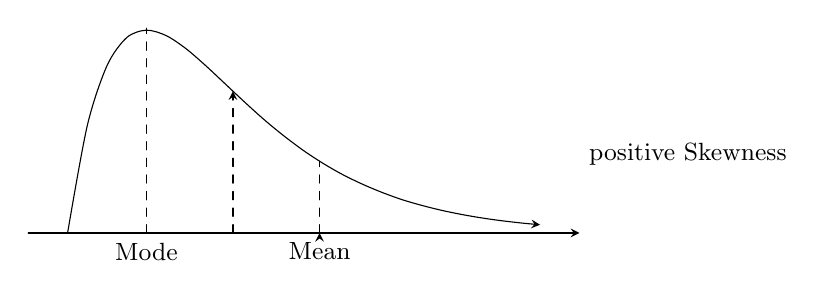
\begin{tikzpicture}[->,>=stealth]
\draw(-0.5,0)--(6.5,0);
\draw[smooth,domain=0:12,scale=0.5,variable=\x]plot(\x,{28*\x*exp(-1/2*\x)/4});
\draw[dashed](1,0)--(1,2.6)
(3.2,0)--(3.2,0.91)
(2.1,0)--(2.1,1.8);
\draw(6.5,1)node[right]{positive Skewness}
(1,0)node[below]{Mode}
(3.2,0)node[below]{Mean};
\end{tikzpicture}
\end{figure}
 
 
 
 
 
 
 
 
 
\vspace{1cm}
 
 
 
% DIAGRAM 11



\begin{figure}[H]
\centering
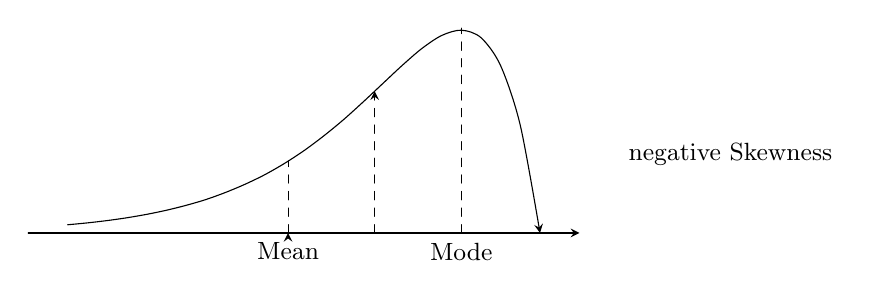
\begin{tikzpicture}[->,>=stealth]
\draw(-6.5,0)--(0.5,0);
\draw[smooth,domain=-12:0,scale=0.5,variable=\x]plot(\x,{-28*\x*exp(1/2*\x)/4});
\draw[dashed](-1,0)--(-1,2.6)
(-3.2,0)--(-3.2,0.91)
(-2.1,0)--(-2.1,1.8);
\draw(1,1)node[right]{negative Skewness}
(-1,0)node[below]{Mode}
(-3.2,0)node[below]{Mean};
\end{tikzpicture}
\end{figure}














Coefficient of skewness measures the degree of lack of symmetry
$$SK=\frac{\text{Mean}\hspace{0.2cm}-\hspace{0.2cm}\text{Mode}}{\sigma}$$\\
$$SK=\frac{3(\text{Mean}\hspace{0.2cm}-\hspace{0.2cm} \text{Median})}{\sigma}$$\\
$$SK=\frac{Q_1+Q_3-2\text{Median}}{Q_3-Q_1}$$\\
$$SK=\frac{\sqrt{\beta_1}(\beta_2+3)}{2(5\beta_2-6\beta_1-a)}$$\\



\textbf{Interpretation}
\begin{enumerate}
\item If $SK=0$, then the distribution  symmetric.
\item If $SK>0$, then the distribution is positively skewed.
\item If $SK<0$, then the distribution is negatively skewed.\\
\end{enumerate}

\textbf{KURTOSIS} is a measure of the degree of peakedness.


% Diagram 12



\begin{figure}[H]
\centering
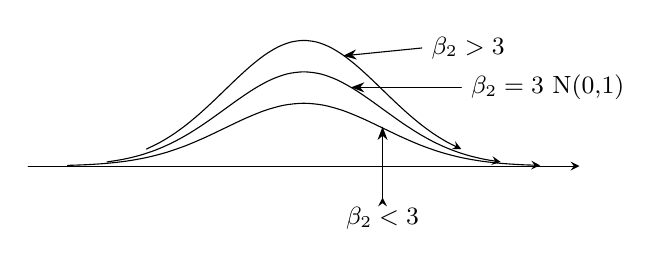
\begin{tikzpicture}[->,>=stealth]
\draw(-3.5,0)--(3.5,0);
\draw[smooth,domain=-3:3,variable=\x]plot(\x,{2*1/sqrt(2*pi)*exp(-1/2*\x*\x)});
\draw[smooth,domain=-2.5:2.5,variable=\x]plot(\x,{3*1/(sqrt(2*pi))*exp(-1/2*\x*\x)});
\draw[smooth,domain=-2:2,variable=\x]plot(\x,{4*1/sqrt(2*pi)*exp(-1/2*\x*\x)});
\draw[-Stealth](1,-0.4)--(1,0.5);
\draw[-Stealth](1.5,1.5)--(0.5,1.4);
\draw[-Stealth](2,1)--(0.6,1);
\draw(1.5,1.5)node[right]{$\beta_2>3$}
(2,1)node[right]{$\beta_2= 3$ N(0,1)}
(1,-0.4)node[below]{$\beta_2<3$};
\end{tikzpicture}
\end{figure}
 

















Coefficient of Kurtosis is calculated as:
$$CK=\frac{\text{Semi Interquartile Range}}{P_{90}-P_{10}}$$
The distribution is normal if $CK=0.263$, otherwise the distribution is not normal.\\\\
\textbf{Example}\\
Given the data below
\begin{table}[h!]
\centering
\begin{tabular}{|c|c|c|}
\hline C-I & $f$ & $X$\\
\hline $0-2$&1&1\\
$2-4$&3&3\\ $4-6$&5&5\\ $6-8$&2&7\\ $8-10$&6&9\\ $10-12$&2&\\ $12-14$&1&\\
\hline
\end{tabular}
\end{table}


Using $a=7$ as un arbitrary value.
\begin{enumerate}
\item Find the first four central moments.
\item Calculate $\beta_1$ and $\beta_2$.
\item Calculate the coefficient of skewness.
\item Calculate the coefficient of Kurtosis.\\
Comment\\
\end{enumerate}















\pagebreak
\subsection{Practice problems}

Past tutorial-sheet questions on sampling and describing data. Try each one before
opening the solution.

\begin{problem}{Tutorial Sheet 1}
Unaware that 45\% of the 20{,}000 voters in his constituency support him, a politician
decides to estimate his political strength. A sample of 200 voters shows that 40\%
support him.
\begin{enumerate}
\item[(a).] What is the population?
\item[(b).] What is the sample?
\item[(c).] What is the parameter of interest? State its value.
\item[(d).] What is the statistic of interest? State its value.
\item[(e).] Compare your answers in (c) and (d). Is it surprising that they differ? If the
politician were to sample another 200 voters, which of the two numbers would be likely to
change? Explain.
\end{enumerate}
\end{problem}

\begin{solution}
\textbf{(a).} The population is all $20{,}000$ voters in the constituency -- every unit we
want a conclusion about, not merely those we happened to ask.

\textbf{(b).} The sample is the $200$ voters actually questioned.

\textbf{(c).} The parameter is the proportion of \emph{all} voters in the constituency who
support him: $p = 0.45$, or $45\%$.

\textbf{(d).} The statistic is the proportion of the \emph{sample} who support him:
$\widehat{p} = 0.40$, or $40\%$.

\textbf{(e).} It is not surprising. A parameter describes the population; a statistic
describes a sample drawn from it. Because the sample is only $200$ of $20{,}000$ voters,
it will rarely reproduce the population proportion exactly, and the gap here -- five
percentage points -- is ordinary sampling variation rather than evidence of a mistake.

If a fresh sample of $200$ were taken, the \textbf{statistic} would almost certainly
change: a different $200$ people give a different count. The \textbf{parameter} would not.
It is a fixed property of the constituency, $0.45$, whether or not anyone measures it.

That asymmetry is the whole basis of what follows in this course. The parameter is fixed
and unknown; the statistic is known and varies. Everything in estimation is an argument
about how far the second can be trusted to say something about the first.
\end{solution}

\begin{problem}{Tutorial Sheet 1}
For the population $\{0,\ 1,\ 2,\ 3,\ 5,\ 7\}$:
\begin{enumerate}
\item[(a).] List all the simple random samples of size 5.
\item[(b).] Give an example of a systematic sample of size 3, where the elements are listed
in the order $0, 1, 2, 3, 5, 7$.
\item[(c).] Give an example of a proportional stratified sample of size 3, where the strata
are $\{0,1,2,3\}$ and $\{5,7\}$.
\item[(d).] Give an example of a cluster sample of size 2, where the clusters are
$\{0,1\}$, $\{2,3\}$ and $\{5,7\}$.
\end{enumerate}
\end{problem}

\begin{solution}
\textbf{(a).} A simple random sample of size 5 is any subset of 5 of the 6 elements, so
there are $\binom{6}{5} = 6$ of them -- one for each element left out:
\[\{0,1,2,3,5\},\quad \{0,1,2,3,7\},\quad \{0,1,2,5,7\},\]
\[\{0,1,3,5,7\},\quad \{0,2,3,5,7\},\quad \{1,2,3,5,7\}.\]

\textbf{(b).} In a systematic sample we take every $k$th element of the ordered list. For a
sample of 3 from 6, $k = 6/3 = 2$. Starting at the first element and taking every second
one gives
\[\{0,\ 2,\ 5\}.\]
Starting at the second instead would give $\{1,3,7\}$; either is a valid answer, and the
starting point should be chosen at random.

\textbf{(c).} Proportional stratified sampling takes from each stratum in proportion to its
size. The strata hold 4 and 2 of the 6 elements, so of a sample of 3 we take
\[\frac{4}{6}\times 3 = 2 \text{ from } \{0,1,2,3\}, \qquad
\frac{2}{6}\times 3 = 1 \text{ from } \{5,7\},\]
choosing at random within each. For example $\{1,\ 3,\ 5\}$.

\textbf{(d).} In cluster sampling we sample \emph{whole clusters}, not individuals. A
sample of size 2 is therefore one entire cluster, for example
\[\{2,\ 3\}.\]
This is the point that separates it from stratified sampling: there, we take some units
from \emph{every} stratum; here, we take \emph{all} units from a few clusters. Stratifying
aims to represent every group; clustering is usually done because reaching a whole group at
once is cheaper.
\end{solution}

\begin{problem}{Tutorial Sheet 1}
The recovery times, in days, for 36 patients are:
\begin{center}
\begin{tabular}{cccccccccccc}
8 & 7 & 6 & 9 & 4 & 5 & 3 & 7 & 8 & 10 & 7 & 7\\
6 & 4 & 10 & 3 & 6 & 8 & 2 & 5 & 4 & 5 & 3 & 8\\
7 & 4 & 6 & 3 & 7 & 12 & 4 & 3 & 6 & 6 & 9 & 4\\
\end{tabular}
\end{center}
\begin{enumerate}
\item[(a).] Construct a frequency distribution.
\item[(b).] What percentage of recovery times are fewer than 6 days?
\item[(c).] Find the mean and median number of days to recovery.
\item[(d).] Find $P_{20}$ and the sample variance $s^{2}$.
\end{enumerate}
\end{problem}

\begin{solution}
\textbf{(a).} Counting each distinct value:
\begin{table}[H]
\centering
\begin{tabular}{lcccccccccc}
Days $x$      & 2 & 3 & 4 & 5 & 6 & 7 & 8 & 9 & 10 & 12\\
\hline
Frequency $f$ & 1 & 5 & 6 & 3 & 6 & 6 & 4 & 2 & 2 & 1\\
\end{tabular}
\end{table}
The frequencies total $36$, which is the first thing to check.

\textbf{(b).} Fewer than 6 days means $x = 2,3,4,5$:
\[1+5+6+3 = 15 \text{ patients}, \qquad \frac{15}{36}\times 100 = 41.67\%.\]

\textbf{(c).} Using $\sum fx$ rather than adding 36 numbers separately:
\[\sum fx = 216, \qquad \bar{x} = \frac{216}{36} = 6 \text{ days}.\]
With $n = 36$ even, the median is the average of the 18th and 19th ordered values. The
cumulative frequencies reach 15 by $x=5$ and 21 by $x=6$, so both the 18th and 19th values
are 6:
\[\text{median} = 6 \text{ days}.\]

\textbf{(d).} $P_{20}$ sits at position $\dfrac{20 \times 36}{100} = 7.2$, that is between
the 7th and 8th ordered values. Cumulatively, 6 observations are at most 3 days and 12 are
at most 4, so the 7th and 8th values are both 4:
\[P_{20} = 4 \text{ days}.\]
For the sample variance, with $\bar{x} = 6$,
\[s^{2} = \frac{\sum f(x-\bar{x})^{2}}{n-1} = \frac{196}{35} = 5.6,
\qquad s = \sqrt{5.6} \approx 2.37 \text{ days}.\]
Note the divisor $n-1$, not $n$: this is a \emph{sample} variance, and dividing by $n$
would underestimate the spread of the population it came from.

That the mean and median are both exactly 6 is a hint about shape -- the distribution is
close to symmetric, which the frequency table bears out: the counts rise to a plateau
around 4 to 7 and fall away on both sides, with one long right tail at 12.
\end{solution}

\begin{problem}{Assignment}
Which of the following variates are discrete and which are continuous?
\begin{enumerate}
\item[(a).] The throw of a die.
\item[(b).] The height of a person.
\item[(c).] The weight of eggs in a basket.
\item[(d).] The number of rooms in a house.
\item[(e).] The age of a car.
\end{enumerate}
\end{problem}

\begin{solution}
The test is whether the possible values can be listed, or whether the variate can take any
value in an interval.
\begin{enumerate}
\item[(a).] \textbf{Discrete} -- only $1,2,3,4,5,6$ are possible.
\item[(b).] \textbf{Continuous} -- height can take any value in a range.
\item[(c).] \textbf{Continuous} -- weight is a measurement.
\item[(d).] \textbf{Discrete} -- a count.
\item[(e).] \textbf{Continuous} -- age is elapsed time, which flows without gaps.
\end{enumerate}
Part (e) is the one that causes argument, because age is usually \emph{stated} as a whole
number of years. But how a value is recorded is not the same as what it can be: a car
three and a half years old has an age, whether or not anybody writes it down that way.
Rounding a measurement does not make the underlying variate discrete -- and the next
question depends on exactly that point.
\end{solution}

\begin{problem}{Assignment}
For the following classes, give the true class limits and the mid-class values.
\begin{enumerate}
\item[(a).] Length in mm, measured to the nearest $0.1$\,mm:
$20.0\text{--}20.4$, $20.5\text{--}20.9$, $21.0\text{--}21.4$, $21.5\text{--}21.9$.
\item[(b).] Length in mm, measured to the nearest $0.01$\,mm:
$20.00\text{--}20.49$, $20.50\text{--}20.99$, $21.00\text{--}21.49$, $21.50\text{--}21.99$.
\item[(c).] Age in years: $1, 2, 3, 4, 5$.
\item[(d).] Weight in kg, to the nearest $1$\,kg: $58, 59, 60, 61, 62, 63$.
\end{enumerate}
\end{problem}

\begin{solution}
A continuous quantity recorded to the nearest unit could really have been anything within
half a unit either side. The \emph{true} class limits stretch the stated ones by that half
unit, so that the classes meet with no gaps between them.

\textbf{(a).} Half of $0.1$ is $0.05$:
\begin{table}[H]
\centering
\begin{tabular}{lcc}
Stated & True limits & Mid-value\\
\hline
$20.0$--$20.4$ & $19.95$--$20.45$ & $20.2$\\
$20.5$--$20.9$ & $20.45$--$20.95$ & $20.7$\\
$21.0$--$21.4$ & $20.95$--$21.45$ & $21.2$\\
$21.5$--$21.9$ & $21.45$--$21.95$ & $21.7$\\
\end{tabular}
\end{table}
Each class ends exactly where the next begins, which is the check that the limits are
right.

\textbf{(b).} Half of $0.01$ is $0.005$, so the limits are $19.995$--$20.495$,
$20.495$--$20.995$, $20.995$--$21.495$ and $21.495$--$21.995$, with mid-values $20.245$,
$20.745$, $21.245$ and $21.745$.

\textbf{(c).} \emph{Age behaves differently, and this is the trap.} Age is not rounded, it
is \emph{truncated}: a person is 1 year old from their first birthday until the day before
their second. So the class ``1'' runs from $1.0$ to $2.0$, not from $0.5$ to $1.5$, and the
mid-value is $1.5$. Likewise the classes are $2.0$--$3.0$, $3.0$--$4.0$, $4.0$--$5.0$ and
$5.0$--$6.0$, with mid-values $2.5$, $3.5$, $4.5$ and $5.5$.

\textbf{(d).} Weight \emph{is} rounded, so the half-unit rule applies again: $57.5$--$58.5$,
$58.5$--$59.5$, and so on up to $62.5$--$63.5$, with mid-values equal to the stated values
$58, 59, \ldots, 63$.

Parts (c) and (d) look alike and are not. Ask how the number was arrived at -- rounded to
the nearest unit, or counted down to the last one completed -- because the mid-values feed
straight into the mean, and getting them half a unit out shifts the answer.
\end{solution}

\begin{problem}{Assignment}
For the data below, give the true class limits, mid-values and relative frequencies.
\begin{table}[H]
\centering
\begin{tabular}{lc}
Height in cm (nearest cm) & Frequency\\
\hline
$120$--$129$ & 2\\
$130$--$139$ & 12\\
$140$--$149$ & 17\\
$150$--$159$ & 18\\
$160$--$169$ & 7\\
$170$--$179$ & 1\\
\end{tabular}
\end{table}
\end{problem}

\begin{solution}
Heights are recorded to the nearest cm, so the true limits run half a centimetre either
side of the stated ones. The frequencies total $n = 57$.
\begin{table}[H]
\centering
\begin{tabular}{lccccc}
Stated & True limits & Mid-value & $f$ & Relative $f$ & Cumulative $f$\\
\hline
$120$--$129$ & $119.5$--$129.5$ & $124.5$ & 2  & $0.035$ & 2\\
$130$--$139$ & $129.5$--$139.5$ & $134.5$ & 12 & $0.211$ & 14\\
$140$--$149$ & $139.5$--$149.5$ & $144.5$ & 17 & $0.298$ & 31\\
$150$--$159$ & $149.5$--$159.5$ & $154.5$ & 18 & $0.316$ & 49\\
$160$--$169$ & $159.5$--$169.5$ & $164.5$ & 7  & $0.123$ & 56\\
$170$--$179$ & $169.5$--$179.5$ & $174.5$ & 1  & $0.018$ & 57\\
\end{tabular}
\end{table}
The relative frequencies sum to 1 and the cumulative frequency ends at 57; both are worth
checking before going further.

For a histogram, the bars are drawn against the \emph{true} limits so that they touch --
gaps between bars would wrongly suggest heights that cannot occur. The cumulative frequency
curve is plotted against the \emph{upper} true limit of each class, since that is the point
by which the accumulated count has been reached.

Using the mid-values, the mean height is estimated as
\[\bar{x} = \frac{\sum fx}{\sum f} = \frac{8426.5}{57} \approx 147.8 \text{ cm}.\]
This is an estimate, not the mean of the original data: once measurements are grouped, the
individual values are gone, and every observation in a class is treated as sitting at its
mid-value.
\end{solution}

\section{Estimation and Sampling Distributions}

\subsection{The Four Distributions You Will Need}

Everything that follows -- confidence intervals, hypothesis tests, analysis of variance,
regression -- is built from four distributions. They are introduced together here because
the hardest part is not the arithmetic but knowing \emph{which one applies}, and that is
easier to see when they are side by side.

\subsubsection{The normal distribution}

A continuous variable $X$ with mean $\mu$ and variance $\sigma^2$ is normal, written
$X\sim N(\mu,\sigma^2)$, if its curve is the familiar symmetric bell centred at $\mu$.
Its properties:
\begin{enumerate}
\item It is symmetric about $\mu$, so mean, median and mode coincide there.
\item The total area under the curve is 1, and $\sigma$ controls the spread -- a larger
$\sigma$ gives a flatter, wider curve.
\item Probabilities are areas: $P(a<X<b)$ is the area under the curve between $a$ and $b$.
\end{enumerate}

There is a different normal curve for every pair $(\mu,\sigma)$, so tables for each are out
of the question. Instead we \textbf{standardise}:
$$Z=\frac{X-\mu}{\sigma} \sim N(0,1).$$
$Z$ counts how many standard deviations a value sits from its mean, which is a pure number
with no units. The \textbf{standard normal} $N(0,1)$ is centred at 0 with
$P(Z<0)=P(Z>0)=0.5$, and it is the one distribution that needs tabulating.

The notation $Z_{\alpha}$ means the value with area $\alpha$ to its \emph{right}, so
$P(Z>Z_{\alpha})=\alpha$. The ones worth knowing by heart are
$$Z_{0.05}=1.645, \qquad Z_{0.025}=1.96, \qquad Z_{0.005}=2.576,$$
which give the $90\%$, $95\%$ and $99\%$ two-sided intervals. Because the curve is
symmetric, $Z_{1-\alpha}=-Z_{\alpha}$ -- one table serves both tails.

\subsubsection{Why the sample mean is normal: the Central Limit Theorem}

The reason the normal distribution dominates a course about \emph{samples} is that
$\overline{X}$ tends to be normal even when the individual observations are not. If a
sample of size $n$ is drawn from a population with mean $\mu$ and variance $\sigma^2$, then
$$E(\overline{X})=\mu, \qquad \operatorname{Var}(\overline{X})=\frac{\sigma^2}{n},
\qquad\text{so}\qquad Z=\frac{\overline{X}-\mu}{\sigma/\sqrt{n}}\sim N(0,1)$$
for large $n$, whatever the shape of the population. In practice $n\geq 30$ is the usual
rule of thumb.

Two consequences worth noticing. The spread of $\overline{X}$ is $\sigma/\sqrt{n}$, not
$\sigma$ -- averages vary less than individual observations, which is why sampling works at
all. And the $\sqrt{n}$ means precision improves slowly: to halve the standard error you
must \emph{quadruple} the sample.

\subsubsection{The $t$-distribution}

The formula above needs $\sigma$, which is almost never known. Replacing it by the sample
value $\widehat{S}$ introduces a second source of variation, and the result is no longer
normal:
$$t=\frac{\overline{X}-\mu}{\widehat{S}/\sqrt{n}} \sim t_{n-1}.$$
Its properties:
\begin{enumerate}
\item It is symmetric about 0, like the standard normal, but with \textbf{heavier tails} --
wider, to pay for the extra uncertainty in estimating $\sigma$.
\item It has one parameter, the \textbf{degrees of freedom}, here $n-1$. One is lost
because $\overline{X}$ had to be estimated before $\widehat{S}$ could be computed.
\item As the degrees of freedom grow, $t$ approaches $N(0,1)$. By about $n=30$ the
difference hardly matters, which is why large-sample work uses $Z$.
\end{enumerate}
So $t_{n-1,\alpha}$ is always a little larger than $Z_{\alpha}$, and confidence intervals
built with $t$ are correspondingly wider. That is not a defect: it is the price of not
knowing $\sigma$.

\subsubsection{The chi-square distribution}

Where the normal and $t$ concern \emph{means}, the chi-square distribution, $\chi^2_{v}$,
concerns \emph{squared} quantities -- variances and counts.
\begin{enumerate}
\item It takes only non-negative values, since it is built from squares, and it is
\textbf{not symmetric}. It is skewed to the right, becoming more symmetric as the degrees
of freedom increase.
\item Because it is not symmetric, the two tails must be looked up \emph{separately}:
$\chi^2_{1-\alpha/2}$ and $\chi^2_{\alpha/2}$ are not negatives of one another, and there
is no shortcut of the kind symmetry allows for $Z$ and $t$.
\end{enumerate}
It appears twice in this course: for inference about a variance, where
$(n-1)\widehat{S}^2/\sigma^2\sim\chi^2_{n-1}$, and in the goodness-of-fit and independence
tests, where the statistic sums squared discrepancies between observed and expected counts.

\subsubsection{The $F$-distribution}

The $F$-distribution arises when \emph{two} variances are compared, as a ratio:
$$F=\frac{\widehat{S}_1^2/\sigma_1^2}{\widehat{S}_2^2/\sigma_2^2}
\sim F_{v_1,\,v_2}.$$
\begin{enumerate}
\item It has \textbf{two} degrees-of-freedom parameters -- numerator $v_1$ and denominator
$v_2$ -- and the order matters: $F_{5,20}$ is not $F_{20,5}$.
\item It is positive and right-skewed, being a ratio of non-negative quantities.
\item Tables usually give only the upper tail. The lower tail is recovered from
$$F_{1-\alpha,\,v_1,v_2}=\frac{1}{F_{\alpha,\,v_2,v_1}},$$
noting that the degrees of freedom swap.
\end{enumerate}
It is used for testing the equality of two variances, and -- as the next chapter shows --
throughout the analysis of variance, where the whole method rests on comparing variation
between groups with variation within them.

\subsubsection{Choosing between them}

\begin{table}[H]
\centering
\begin{tabular}{lll}
Question & Distribution & Degrees of freedom\\
\hline
A mean, $\sigma$ known & $Z$ & --\\
A mean, $\sigma$ unknown & $t$ & $n-1$\\
A proportion, $n$ large & $Z$ & --\\
A single variance & $\chi^2$ & $n-1$\\
Two variances compared & $F$ & $v_1, v_2$\\
Counts against expected counts & $\chi^2$ & $k-1-m$ or $(r-1)(c-1)$\\
Several means compared & $F$ & $k-1,\ n-k$\\
\end{tabular}
\end{table}

\begin{align*}
\textbf{Notation:} & \\ 
\overline{X}&=\hspace{0.3cm}\text{Sample Mean}\\
S^2&=\hspace{0.3cm}\text{Sample Variance}\\
S&=\hspace{0.3cm}\text{Sample s.d.}\\
\mu &=\hspace{0.3cm}\text{Population Mean}\\
\sigma^2&=\hspace{0.3cm}\text{Population Variance}\\
\sigma &=\hspace{0.3cm}\text{Population s.d.}\\
\end{align*}



We have the theory of probability and now we want the objective of statistics.\\\\ Statistics is about making inference about a population based on information contained in a sample.\\ Generally, population are characterized by numerical descriptive measures and the objective of many investigation is to make an inference about one or more population parameters\\\\ Methods of making inference about population parameters falls in one of two categories:
\begin{enumerate}
\item estimation of parameters.
\item decision making concerning the value of the parameter.\\
\end{enumerate}
Methods of estimation can be classified into:
\begin{enumerate}
\item point estimation
\item interval estimation\\
\end{enumerate}
A point estimation procedure utilize information in a sample to arrive at s single number or point which estimates the target population.\\




\textbf{Definition}\\
An estimate is a rule that tells how to calculate an estimate and on the measurement contained in a sample.\\

In a point estimation we find a single point or single value to estimate a certain unknown parameter say $\theta$. (Point estimate of a population parameter is a value of the corresponding sample statistic)\\

The procedure used to find such a value is called an estimation usually denoted by $\widehat{\theta}$.\\

Interval estimate, and interval is constructed around the point estimate, and it is stated that this interval is likely to contain the corresponding population parameter.\\







\begin{center}
 \subsubsection{{Properties of Estimation}}
\end{center}
Suppose we want to estimate a population parameter $\theta$. The estimation of $\theta$ will be indicated by the symbol $\widehat{\theta}$. We would like the distribution of estimates of the probability distribution of the estimation to center about the target parameters.




% Diagrm 13

\begin{figure}[H]
\centering
\begin{tikzpicture}[->,>=stealth]
\draw(-3.5,0)--(3.5,0);
\draw[smooth,domain=-3:3,variable=\x]plot(\x,{6*1/sqrt(2*pi)*exp(-1/2*\x*\x)});
\draw[dashed](0,0)--(0,2.39);
\draw(0,0)node[below]{$E(\widehat{\theta})$}
(-1.5,0)node[below]{$\theta$};
\draw[dashed](-1.5,0)--(-1.5,0.75);
\end{tikzpicture}
\end{figure}














Probability distribution for a positively biased estimator.\\


\textbf{Definition}\\
Let $\widehat{\theta}$ be an estimation of the parameter $\theta$. Then $\widehat{\theta}$ is an unbiased estimator if $E(\widehat{\theta})=\theta$. Otherwise, $\widehat{\theta}$ is said to be biased.\\



\textbf{Definition}\\
The bias $B$ of an estimator $\widehat{\theta}$ is given by $B=E(\widehat{\theta})-\theta$.\\ 

In addition to unbiasedness we like the spread of a distribution of estimation to be as small as possible. That is, we want var$(\widehat{\theta})$ to be a minimum. Given two unbiased estimators of a parameter $\theta$, and all other things equal, we would select the estimator with a small variance other than the biased and variance to determine goodness of an estimation, we can also look at the expected value of $(\widehat{\theta}-\theta)^2$ the square of distance between $\widehat{\theta}$ and the target parameters.\\



\textbf{Definition}\\
Then mean square error of an estimator $\widehat{\theta}$ is defined to be the expected value of $(\widehat{\theta}-\theta)^2$
\begin{align*}
\text{MSE}(\widehat{\theta}) &=E(\widehat{\theta}-\theta)^2\\
&=\text{var}(\widehat{\theta})+B^2
\end{align*}





\textbf{Example}\\
Suppose a population consists of $\{2,4,6\}$ values. Take all sample of size 2 which can be drawn.
\begin{enumerate}
\item Without replacement (combinations).
\item With replacement
\end{enumerate}
Estimate the populations mean and variance.\\


\textbf{Solution}
\begin{enumerate}
\item The number of sample that can be drawn is $
\begin{pmatrix}
3\\2\\
\end{pmatrix}
=3$.
\begin{table}[H]
\centering
\begin{tabular}{c|c|c}
Samples &$\overline{X}$&\\
\hline 2\,,\,4&3&$\overline{X}_1$\\2\,,\,6&4&$\overline{X}_2$\\4\,,\,6&5&$\overline{X}_3$\\
\end{tabular}
\hspace{1cm}
$E(\overline{X})=\mu \implies \mu =\dfrac{2+3+6}{3}=4$\\
\end{table}




\begin{table}[H]
\centering
\begin{tabular}{c|c}
$X$&$(X-\overline{X})^2$\\
\hline 2&4\\ 4&0\\ 6&4\\
\hline &8\\
\end{tabular}
\hspace{1cm}
$\sigma^2=\frac{\sum (X-\overline{X})^2}{n}=\dfrac{8}{3},\hspace{1cm} E(S^2)=\sigma^2$
\end{table}


\begin{align*}
E(\widehat{\overline{X}} &=\frac{\overline{X}_1+\overline{X}_2+\overline{X}_3}{3}=\frac{3+4+5}{3}\\\\
\implies\hspace{1cm} E(\widehat{\overline{X}})&=4
\end{align*}


$\therefore$ Sampling without replacement $E(\widehat{\overline{X}})=\mu$.\\


\item Samples with replacement $=(N)^n=3^2=9$ samples
\begin{table}[H]
\centering
\begin{tabular}{c|c|c}
Samples & $\overline{X}$&\\
\hline 2\,,\,2 &2&$\overline{X}_1$\\2\,,\,4&3&$\overline{X}_2$\\2\,,\,6&4&$\overline{X}_3$\\4\,,\,2&3&$\overline{X}_4$\\4\,,\,4&4&$\overline{X}_5$\\4\,,\,6&5&$\overline{X}_6$\\6\,,\,2&4&$\overline{X}_7$\\6\,,\,4&5&$\overline{X}_8$\\6\,,\,6&6&$\overline{X}_9$
\end{tabular}
\end{table}

\begin{align*}
E(\widehat{\overline{X}}) &=\frac{\overline{X}_1+\overline{X}_2+\dots \overline{X}_9}{9}\\\\ &=\frac{2+3+4+3+5+5+4+6}{9}\\ \implies \hspace{0.5cm} E(\widehat{\overline{X}}) &=4\\
\end{align*}
$\therefore$ Sampling with replacement of $E(\widehat{\overline{X}})=\mu$.\\\\
$\therefore$ The sample mean is an unbiased estimator of the population mean $E(\widehat{\overline{X}})=\mu$.\\\\
$$S^2=\frac{\sum (X-\overline{X})^2}{n},\hspace{1cm} S^2=\frac{\sum (X-\overline{X})^2}{n-1}$$\\



\begin{table}[H]
\centering
\begin{tabular}{|c|c|c|c|}
\hline
Samples &$\overline{X}$&$S^2=\dfrac{\sum (X-\overline{X})^2}{n-1}$&$S^2=\dfrac{\sum (X-\overline{X})^2}{n}$\\
\hline 
&&$S^2_1=\dfrac{(2-3)^2+(4-3)^2}{2-1}$&$S^2_1=\dfrac{(2-3)^2+(4-3)^2}{2}$\\
\hline 
2\,,\,4&3&&\\
2\,,\,6&4&&\\ 4\,,\,6&5&&\\
\hline
\end{tabular}
\end{table}
\end{enumerate}


\vspace{0.2cm}



\begin{enumerate}
\item Without replacement:\hspace{0.3cm} $E(\widehat{S}^2) =\dfrac{S_1^2+S_2^2+S_3^2}{N}=\dfrac{2+8+2}{3}$
$$\implies\hspace{0.5cm} E(\widehat{S}^2)=4$$



\item With replacement
\begin{align*}
E(\widehat{S}^2) &=\frac{S_1^2+S_2^2+........+S_9^2}{9}=\frac{0+2+8+2+0+2+8+2+0}{9}=\frac{24}{9}\\
\implies\hspace{0.5cm} E(\widehat{S}^2) &=\frac{8}{3}
\end{align*}
\end{enumerate}

Sampling with replacement the $\widehat{S}^2=\dfrac{\sum (X-\overline{X})^2}{n-1}$ is an unbiased estimator of the population variance.\\
 
However, sampling without replacement will give us an unbiased estimation of $\sigma^2$ for\\ $\widehat{S}^2=\dfrac{\sum (X-\overline{X})^2}{n-1}$ because there exist a factor $\dfrac{n-1}{n-1}$ which can be multiplied to $\widehat{S}^2$ to give us an unbiased estimator of $\sigma^2$.\\\\
$\widehat{S}^2=\dfrac{n-1}{n}\,\cdot \,4$,  $n=2$ sample size.\\\\
By the central limit theorem, The sampling distribution of the mean tends to Normal distribution as $n\longrightarrow N$
$$\widehat{S}^2=\frac{N-1}{N}\,\cdot \,4=\frac{3-1}{3}\,\cdot\,4=\frac{8}{3},\hspace{0.6cm}\implies E(\widehat{S}^2)=\sigma^2$$\\

\textbf{Theorem}\\
If all possible random samples, size $n$ are drawn (with replacement) from a population mean $\mu$ and s.d. $\sigma$, then the mean of the samples  have a probability distribution known as sampling distribution of the mean with mean $\mu$ and s.d. $\sigma /\sqrt{n}$.\\ The s.d. of the sampling distribution of the mean is known as the standard error $(s.e)$ of the mean.\\\\





\pagebreak
\textbf{Proof}\\
We know that $E(X)=\mu$ and $E(X)$ is the mean of the sampling distribution of the mean. Therefore, the variance of sampling distribution is var$(\overline{X})$.
\begin{align*}
\text{var}(\overline{X}) &=\text{var}\Bigg\{\frac{\sum X}{n}\Bigg\}=\frac{1}{n^2}\,\,\text{var}\Bigg\{\sum X \Bigg\}\\
&=\frac{1}{n^2}\,\{\text{var}(X_1)+\text{var}(X_2)+............+\text{var}(X_n)\}
=\frac{1}{n^2}\hspace{0.1cm}\cdot\hspace{0.1cm}n\sigma^2\\
&=\frac{\sigma^2}{n}.
\end{align*}
\begin{equation}\label{eq:var-xbar}
\operatorname{var}(\overline{X})=\frac{\sigma^2}{n}
\end{equation}
$$\text{The s.e}=\frac{\sigma}{\sqrt{n}}\hspace{0.3cm}\text{of the sampling distribution of means.}$$
If the sampling is without replacement from a population of size $N$, the variance acquires
a \textbf{finite population correction}:
% This read (N-n)/(N-n), which is 1 and so corrects nothing. The correction
% factor is (N-n)/(N-1).
\begin{equation}\label{eq:var-xbar-fpc}
\operatorname{var}(\overline{X})=\frac{\sigma^2}{n}\left(\frac{N-n}{N-1}\right)
\end{equation}
The factor is less than 1, so sampling without replacement gives a \emph{more} precise mean
than sampling with replacement -- each observation drawn is one that cannot be drawn again,
so the sample carries more information about the population. If $n$ is very much smaller
than $N$ the factor is close to 1 and \eqref{eq:var-xbar-fpc} gives approximately
\eqref{eq:var-xbar}. In the extreme case $n=N$ the whole population has been measured, the
factor is 0, and there is no sampling error at all -- which is exactly as it should be.\\ Whether the sampling is with or without replacement var$(\overline{X})$ decreases as the sample size increases.\\ That means the lager the sample size the closer the sample mean is likely to the population mean
% These were both written as E(S^2) = ..., but they are definitions of the
% estimator, not its expectation.
$$S^2=\frac{\sum (X-\mu)^2}{n}\hspace{1cm}\text{(unbiased, but needs }\mu\text{)}$$
$$S^2=\frac{\sum (X-\overline{X})^2}{n}\hspace{1cm}\text{(biased)}$$

However, $S^2=\dfrac{\sum (X-\overline{X})^2}{n}$ is not an unbiased estimator of population variance.\\\\ We want to find an unbiased estimator of $\sigma^2$
\begin{align*}
\sigma^2 &=E\Bigg[\frac{\sum (X-\mu)^2}{n}\Bigg]=E\Bigg[\frac{\sum\Big\{(X-\overline{X})-(\mu -\overline{X)}\Big\}^2}{n}\Bigg]\\\\
&=E\Bigg[\frac{\sum [(X-\overline{X})^2-2(X-\overline{X})(\mu-\overline{X})+(\mu -\overline{X})^2]}{n}\Bigg]\\\\
&=E\Bigg[\frac{\sum (X-\overline{X})^2}{n}-\frac{2(\mu-\overline{X})\sum (X-\overline{X})}{n}+\frac{\sum (\mu-\overline{X})^2}{n}\Bigg]\\\\
&=E\Bigg[\frac{\sum (X-\overline{X})^2}{n}\Bigg]+E(\mu-\overline{X})^2\\\\ \implies\hspace{0.5cm} \sigma^2 &=E(S^2)+E(\mu-\overline{X})^2\\
\end{align*}
The second term $E(\mu-\overline{X})^2$ is var$(\overline{X})$. i.e. var$(\overline{X})=\dfrac{\sigma^2}{n}.$

\begin{align*}
\sigma^2 &=E(S^2)+\frac{\sigma^2}{n}\hspace{0.5cm}\implies\hspace{0.5cm} \sigma^2-\frac{\sigma^2}{n}=E(S^2)\\\\
\sigma^2\frac{(n-1)}{n}&=E(S^2)\hspace{0.5cm}\implies\hspace{0.5cm} \sigma^2=\frac{n}{n-1}E(S^2)\\\\
\sigma^2 &=\frac{n}{n-1}(E(S^2))\\\\ \sigma^2 &=\frac{n}{n-1}\Bigg(\frac{\sum (X-\overline{X})^2}{n}\Bigg)\\\\ \sigma^2 &=E\Bigg(\frac{\sum (X-\overline{X})^2}{n-1}\Bigg)\\\\ \implies\hspace{0.5cm} \sigma^2&=E(\widehat{S}^2)\\
\end{align*}
This gives us unbiased estimator of variance, it is denoted by $\widehat{S}^2$ $$\therefore\hspace{0.3cm} \widehat{S}^2=\frac{\sum (X-\overline{X})^2}{n-1}$$ and $\widehat{S}^2$ and $S$ are related by \hspace{0.2cm}$\displaystyle{\widehat{S}^2=\frac{n}{n-1}S^2,\hspace{1cm} \sigma^2=\widehat{S}^2}$\\

The term $n-1$ is called the degree of freedom an its symbol is $v$. Degrees of freedom means if we know $\mu$, then the variance can be calculated from $n$ independent deviation using $\dfrac{\sum (X-\mu)^2}{N}$\,, if instead we measure the deviation from $\overline{X}$, then we have only $n-1$ independent deviations can be deduced from the fact that $\sum (X-\overline{X})=0$. One d.f has to be lost since only $n-1$ of the deviation can be varied independently.\\













\begin{center}
\subsubsection{An Unbiased Estimation of Population Proportion}
\end{center}
If the probability that a member of a population posses an attributes $P$, then we know that $X$ the number of members of sample size $n$ which possess this attribute is Binomially distributed $B(n,P)$, we expect $P_s=X/n$.\\ The proportion in the sample which shows the attribute to be an unbiased estimator of $P$ and we can show it as;
\begin{align*}
E(P_s) &=E(X/n)=\frac{1}{n}E(X)\\
&=\frac{1}{n}\hspace{0.1cm}\cdot\hspace{0.1cm} nP\\\\
\implies\hspace{0.5cm} E(P_s) &=P\\
\end{align*}
$E(P_s)=P\implies P_s$ is an unbiased estimator of the population proportion $P$.\\\\ We can also find the value of the sampling distribution of $P_s$ since
\begin{align*}
\text{var}(P_s) &=\text{var}(X/n)=\frac{1}{n^2}\text{var}(X)\\ &=\frac{1}{n^2}\hspace{0.1cm} nP(1-P)\\\\ \implies\hspace{0.5cm} \text{var}(P_s) &=\frac{P(1-P)}{n}\\
\end{align*}
when $n$ is large the sampling distribution of $X$ tends to a normal distribution. Thus, the sampling distribution of $P_s$ tends to $N(0,1)$ with mean $X/n$ and variance $\dfrac{P(1-P)}{n}$ and standard error of proportion as $\sqrt{\dfrac{P(1-P)}{n}}$.\\\\\\




\subsubsection{Expected Values And Variances of Some Common Point Estimators}


\begin{table}[H]
\centering
\begin{tabular}{|c|c|c|c|c|}
\hline Target & Sample & Point & Expected & Variance\\
Parameter & size & estimator & value &\\
$\theta$ & $n$ & $\widehat{\theta}$ & $\widehat{\theta}$ & $\widehat{\theta}$\\
\hline $\mu$ & $n$ & $\overline{X}$ & $\mu$ & $\sigma^2/n$\\
$P$ & $n$ & $\widehat{P}=X/n$ & $P$ & $Pq /n$\\
$\mu_1-\mu_2$ & $n_1\, \&\, n_2$ & $\overline{X}_1-\overline{X}_2$ & $\mu_1-\mu_2$& $\dfrac{\sigma^2_1}{n_1}+\dfrac{\sigma^2_2}{n_2}$\\
$P_1-P_2$ & $n_1\,\&\, n_2$ & $\widehat{P}_1-\widehat{P}_2$ & $P_1-P_2$ & $\dfrac{P_1q_1}{n_1}+\dfrac{P_2q_2}{n_2}$\\
\hline
\end{tabular}
\end{table}



\vspace{0.3cm}
\textbf{Definition}\\
The error of estimation $\epsilon$ is the distance between an estimator and its target parameter, that is $\epsilon =|\widehat{\theta}-\theta|$.



% Diagram 14


\begin{figure}[H]
\centering
\begin{tikzpicture}[->,>=stealth]
\draw[-Stealth](-3.4,-0.5)--(-3.4,2.8)node[above]{$\epsilon(\theta)$};
\draw[-Stealth](-3.5,0)--(3.8,0)node[right]{$\widehat{\theta}$};
\draw[smooth,domain=-3.5:3.5,variable=\x]plot(\x,{6*1/sqrt(2*pi)*exp(-1/2*\x*\x)});
\draw[dashed](0,0)--(0,2.39)
(-1.5,0)--(-1.5,0.75)
(1.5,0)--(1.5,0.75);
\draw(-1.5,0)node[below]{$\theta-b$}
(0,0)node[below]{$\theta$}
(1.5,0)node[below]{$\theta + b$}
(0,1)node[above]{$P(\epsilon > b)$};
\end{tikzpicture}
\end{figure}












The probability distribution of an estimator $\widehat{\theta}$, whether we know the probability distributes of $\widehat{\theta}$ or not; an approximated bound on $\epsilon$ for unbiased estimators can be found by expressing $b$ as a multiple s.d. of $\widehat{\theta}$ say $b=k\sqrt{\widehat{\theta}}$ and the default for $k=2$, $b=2\sqrt{\widehat{\theta}}$.\\








\textbf{Examples}
\begin{enumerate}
\item A sample of $n=1000$ voters randomly selected a city showed $Y=560$ in favor of candidate $A$. Estimate the fraction of votes in the population favoring $A$, $P$ and place a bound on the error of estimation.
\item Five measurements of the volume of acid required in a titration are; 25.1, 25.2, 25.2, 25.0, 25.5 cm$^3$.\\ Use these results to obtain estimation for the mean and s.d. of the volume required.\\
\end{enumerate} 




\textbf{Solutions}
\begin{enumerate}
\item This is a proportion question and we want to estimate $P$. \hspace{0.2cm}$P_s=Y/n$\, we use $P_s$ to estimate.\\

$\therefore$ The estimate of $P$ i.e. fraction of voters following candidate $A$ is $$P_s=Y/n=\frac{560}{1000}=0.56$$ $56\%$ of the population favored candidate $A$.\\ 
The probability distribution of $P_s$ will be approximated by the normal distribution because $n=1000$. Large or small is $n=30$. If $n\geq 30$, it is assumed $N(0,1)$ large sample size.\\ 

If $n<30$ - small sample size. $P_s=P$ because $P_s$ is an unbiased estimator.\\ 

$\therefore$ we want $b=2\sqrt{\widehat{\theta}}\hspace{0.6cm}\implies b=2\sqrt{\dfrac{Pq}{\sigma}}$.\\ 

Binomial distribution  s.e $=\sqrt{\dfrac{Pq}{n}}$. $$b=2\sqrt{\frac{(0.56)(0.44)}{1000}}=0.03$$
$\therefore$ The probability that the error of estimation is less than 0.03 is approximately 0.95, we are confident that our estimate of 0.56 is within 0.03 of the population value of $P$. \,$(95\%\hspace{0.3cm}\text{confident})$,$$0.56-0.03<P<0.56+0.03$$\\

\begin{table}[H]
(2)$\hspace{3cm}$
\centering
\begin{tabular}{|c|c|c|c|c|}
\hline 
$X$ & $f$ & $f(X)$ & $X-\overline{X}$ & $(X-\overline{X})^2$\\
\hline 25.1&1&25.1& $-0.1$ & 0.01\\
25.2& 2& 50.4&0&0\\
25.0 &1& 25.0& $-0.2$& 0.04\\
25.5&1&25.5&0.3&0.09\\
\hline &5&126.0&&0.14\\
\hline
\end{tabular}
\end{table}



\begin{align*}
\overline{X} &=\frac{\sum f(X)}{\sum f}=\frac{126}{5}\\ &=25.2\hspace{0.2cm}\text{cm}^2\\\\
\therefore \hspace{0.5cm} E(\overline{X})&=\mu=25.2\text{cm}^2\\
\end{align*}
$E(\overline{X})$ is an unbiased estimator of population mean, $E(\overline{X})=\mu$.\\
$$S^2=\frac{\sum (X-\overline{X})^2}{n}\hspace{1cm}\text{or}\hspace{1cm} \widehat{S}^2=\frac{\sum (X-\overline{X})^2}{n-1}$$
\begin{align*}
\widehat{S}^2 &=\frac{0.14}{4}=0.035\hspace{1cm}\implies \widehat{S}=\sqrt{0.035}\\\\
E(\widehat{S}) &=\frac{\widehat{S}}{\sqrt{n}}=\frac{\sqrt{0.035}}{\sqrt{5}}=0.083666002\approx 0.084\\
\end{align*}
The other formula $E(\widehat{S})=\dfrac{S}{\sqrt{n-1}}$\\ $$\epsilon \hspace{0.5cm} \text{at}\hspace{0.5cm} b=2\times \sqrt{\frac{0.035}{5}}$$\\
\end{enumerate}










\subsubsection{Confidence Interval}
An interval estimate gives a range of values which has a certain probability of containing the population parameter. We find the interval estimates for population mean $\mu$ where $\sigma=$ unknown or $\sigma=$ unknowing.\\ Also we consider the sample size $n\geq 30$ is called large sample size and we use $Z$ - table.\\ We can use this distribution to find a range of the value for which $\overline{X}$ will lie within a certain probability.



% Diagram 15

\begin{figure}[H]
\centering
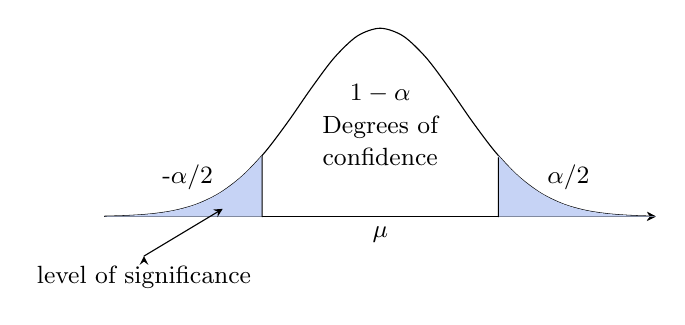
\begin{tikzpicture}[->,>=stealth]
\draw(-3.5,0)--(3.5,0);
\draw[smooth,domain=-3.5:3.5,variable=\x]plot(\x,{6*1/sqrt(2*pi)*exp(-1/2*\x*\x)});
\path[fill=blue!25, smooth, domain=1.5:3.5, variable=\x]plot(\x,{6*1/sqrt(2*pi)*exp(-1/2*\x*\x)})--(3.5,0)--(1.5,0)--(1.5,0.75);
\path[fill=blue!25, smooth, domain=-3.5:-1.5, variable=\x]plot(\x,{6*1/sqrt(2*pi)*exp(-1/2*\x*\x)})--(-1.5,0.75)--(-1.5,0)--(-3.5,0);
\draw(-1.5,0)--(-1.5,0.77)
(1.5,0)--(1.5,0.75)
(-3,-0.5)--(-2,0.1);
\draw(0,0)node[below]{$\mu$}
(0,1.8)node[below]{$1-\alpha$}
(0,1.4)node[below]{Degrees of}
(0,1)node[below]{confidence}
(-2,0.5)node[left]{-$\alpha/2$}
(2,0.5)node[right]{$\alpha/2$}
(-3,-0.5)node[below]{level of significance};
\end{tikzpicture}
\end{figure}





















$\alpha=$ proportion of missing the correct value. $\alpha$ level of significance.\\\\ Our confidence interval is given by: \hspace{0.2cm}$\overline{X}\pm Z_{\alpha/2}\times \text{SE}$

\begin{align*}
\overline{X} &=\hspace{0.3cm} \text{Sample mean}\\
Z_{\alpha/2} &=\hspace{0.3cm}\text{degree of confidence table value with given}\hspace{0.2cm}\alpha.\\
\text{SE} &=\hspace{0.3cm}\text{Standard error}\\
\end{align*}







\subsubsection{Properties of Confidence Intervals}

Which multiplier to use, $Z$ or $t$, is decided by one question only: \textbf{is $\sigma$
known?} It is \emph{not} decided by the sample size. The $t$-distribution exists because
replacing $\sigma$ by an estimate $\widehat{S}$ adds a second source of uncertainty, and
$t$ is wider than $Z$ to pay for it. If $\sigma$ is genuinely known there is nothing extra
to pay for, so $Z$ is correct however small the sample.

Sample size decides something different: whether the interval is trustworthy at all. For
small $n$ these formulas need the population to be roughly normal; for large $n$ the
Central Limit Theorem makes that assumption unnecessary.

\begin{enumerate}
\item $\sigma$ known, any $n$ (population normal, or $n$ large):
$$\overline{X}\pm Z_{\alpha/2}\times \frac{\sigma}{\sqrt{n}}$$

\item $\sigma$ unknown, $n$ large:
$$\overline{X}\pm Z_{\alpha/2}\times \frac{\widehat{S}}{\sqrt{n}}
\hspace{0.5cm}\text{equivalently}\hspace{0.5cm}
\overline{X}\pm Z_{\alpha/2}\times \frac{S}{\sqrt{n-1}}$$
The two forms agree because $S$ is computed with divisor $n$ and $\widehat{S}$ with
divisor $n-1$, so $\widehat{S}/\sqrt{n}=S/\sqrt{n-1}$. Strictly $t$ is correct here too,
but for large $n$ the two are indistinguishable.

\item $\sigma$ unknown, $n$ small (population normal):
$$\overline{X}\pm t_{n-1,\,\alpha/2}\times \frac{\widehat{S}}{\sqrt{n}}
\hspace{0.5cm}\text{equivalently}\hspace{0.5cm}
\overline{X}\pm t_{n-1,\,\alpha/2}\times \frac{S}{\sqrt{n-1}}$$
This is the only case that calls for $t$.

\item C.I.\ for a proportion, $n$ large enough that $n\widehat{P}\geq 5$ and
$n(1-\widehat{P})\geq 5$:
$$\widehat{P}\pm Z_{\alpha/2}\times \sqrt{\frac{\widehat{P}(1-\widehat{P})}{n}}$$
Note it is the \emph{sample} proportion $\widehat{P}$ throughout: if $P$ were known there
would be nothing to estimate. When the sample is too small for that condition, $t$ does
\textbf{not} rescue it -- a proportion is a count from a binomial, and there is no
estimated variance for $t$ to correct. The proper remedies are the Wilson score interval
or the exact Clopper--Pearson interval, both beyond this course.

\item C.I.\ for the difference between two means, $\sigma_1$ and $\sigma_2$ known:
$$(\overline{X}_1-\overline{X}_2)\pm Z_{\alpha/2}\times
\sqrt{\frac{\sigma_1^2}{n_1}+\frac{\sigma_2^2}{n_2}}$$

\item C.I.\ for the difference between two proportions:
$$(\widehat{P}_1-\widehat{P}_2)\pm Z_{\alpha/2}\times
\sqrt{\frac{\widehat{P}_1(1-\widehat{P}_1)}{n_1}+\frac{\widehat{P}_2(1-\widehat{P}_2)}{n_2}}$$

\item C.I.\ for the difference between two means when $\sigma_1=\sigma_2$ but both are
unknown. The two samples are pooled into a single estimate of the common standard
deviation:
$$(\overline{X}_1-\overline{X}_2)\pm t_{n_1+n_2-2,\,\alpha/2}\times
S_p\sqrt{\frac{1}{n_1}+\frac{1}{n_2}}
\hspace{0.4cm}\text{where}\hspace{0.4cm}
S_p=\sqrt{\frac{(n_1-1)\widehat{S}^2_1+(n_2-1)\widehat{S}^2_2}{n_1+n_2-2}}$$
The multiplier is $t$, not $Z$, because $\sigma$ is unknown -- the same rule as case 3 --
and the degrees of freedom are $n_1+n_2-2$, one lost from each sample. Pooling is only
reasonable if the two variances really are close; a common rough check is
$$\frac{1}{2}<\frac{\widehat{S}^2_1}{\widehat{S}^2_2}<2.$$
\end{enumerate}







\begin{enumerate}
\item[$\bullet$] The number we add to and subtract from the point estimate is called the ``margin of error".
$$\text{Point estimate}\, \pm \, \text{Margin error}$$
confidence level is denoted by $\hspace{0.2cm}(1-\alpha)\, 100\%$
\item[$\bullet$] Margin of error for the estimate for $\mu$ denoted by $E$, is the quantity that is subtracted from and added to the value of $\overline{X}$ to obtain a confidence interval for $\mu$. Thus $$E = Z\,\cdot\,\sigma_{\overline{X}} = Z\,\cdot \, \dfrac{\sigma}{n}$$\\
\end{enumerate}











\textbf{Example}
\begin{enumerate}
\item The s.d. for a method of measuring the concentration of nitrate ions in water is known to be 0.05 PPM. If 100 measurements give a mean of 1.13 PPM. Calculate the $95\%$ confidence interval for the true mean.
\item Fifty children were selected at random from the pupils at a school and each was asked how many hours he/she spent watching TV. The mean of the sample was 17.2 hrs and the s.d. was 5.3 hrs. Calculate $95\%$ confidence interval for the mean number of hrs spent a week watching TV for the population of all children in the school.
\item The masses in grams of thirteen ball bearings taken at random from a batch are:



\begin{table}[H]
\centering
\begin{tabular}{ccccccc}
21.4, &23.1,& 25.9,& 24.7,& 23.4,& 24.5, & 25.0\\ 22.5,&26.9,&26.4,&25.8,& 23.2,&21.9&\\
\end{tabular}
\end{table}

Calculate $99\%$ C.I for the mean mass of the population supposed normal from which there masses where drawn.
\item Out of a random sample of 50 children from a school, 24 where found to have being vaccinated against whoop cough. Calculate the $95\%$ C.I for the proposition of children of the school who have been vaccinated against whoop cough.
\item Mothers breast milk includes Calcium some of that Calcium comes from the food the mother eat and some comes from the mothers bones.\\ Research measured the percent change in Calcium content in the spines of a random sample of 47 mothers during the three months of breast feeding immediately after the baby was born. Calculate $95\%$ C.I of the percent change Calcium level for the population of nursing mothers.\\
\end{enumerate}

\textbf{Solutions}
\begin{align*}
(1)\hspace{0.5cm}\hspace{0.5cm} \text{Given}\hspace{0.3cm} \sigma &=0.05\hspace{0.2cm}\text{PPM}\hspace{0.3cm} (\sigma =\hspace{0.3cm}\text{known) large sample size}\\
n&=100\\ \overline{X}&=1.13\hspace{0.2cm}\text{PPM}\\\\
\overline{X} &\pm Z_{\alpha/2}\hspace{0.1cm}.\hspace{0.1cm}\text{SE}\hspace{0.5cm}\implies \hspace{0.5cm} \overline{X}\pm Z_{\alpha/2}\hspace{0.1cm}.\hspace{0.1cm}\frac{\sigma}{\sqrt{n}}\\\\
Z_{0.025}&=1.96
\end{align*}



% Diagram 16

\begin{figure}[H]
\centering
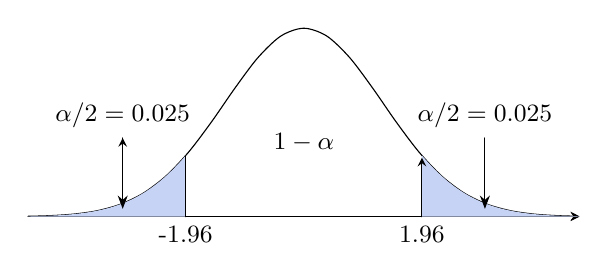
\begin{tikzpicture}[->,>=stealth]
\draw(-3.5,0)--(3.5,0);
\draw[smooth,domain=-3.5:3.5,variable=\x]plot(\x,{6*1/sqrt(2*pi)*exp(-1/2*\x*\x)});
\path[fill=blue!25, smooth, domain=1.5:3.5, variable=\x]plot(\x,{6*1/sqrt(2*pi)*exp(-1/2*\x*\x)})--(3.5,0)--(1.5,0)--(1.5,0.75);
\path[fill=blue!25, smooth, domain=-3.5:-1.5, variable=\x]plot(\x,{6*1/sqrt(2*pi)*exp(-1/2*\x*\x)})--(-1.5,0.75)--(-1.5,0)--(-3.5,0);
\draw(-1.5,0)--(-1.5,0.77)
(1.5,0)--(1.5,0.75);
\draw(-1.5,0)node[below]{-1.96}
(0,1.18)node[below]{$1-\alpha$}
(1.5,0)node[below]{1.96}
(2.3,1)node[above]{$\alpha/2=0.025$}
(-2.3,1)node[above]{$\alpha/2=0.025$};
\draw[-Stealth](-2.3,1)--(-2.3,0.1);
\draw[-Stealth](2.3,1)--(2.3,0.1);
\end{tikzpicture}
\end{figure}



















\begin{align*}
P(Z>Z_1) &=0.025\\ 1.13&\pm 1.96\times \frac{0.05}{\sqrt{100}}\hspace{0.5cm}\implies\hspace{0.5cm} 1.13\pm 1.96\times \frac{0.05}{10}\\
1.13 &\pm 0.0098\\\\
1.13-0.0098\leq &\mu \leq 1.13+0.0098\\
\implies\hspace{0.5cm} 1.1202\leq &\mu \leq 1.1398
\end{align*}
we are $95\%$ confident that the true mean lie in the interval as $[1.1202,1.1398]$\\\\

$$(2). \hspace{1cm} n=13,\hspace{0.5cm} <30,\hspace{0.5cm} \overline{X}=\frac{\sum X}{n}, \hspace{0.5cm} S=\frac{\sqrt{\sum (X-\overline{X})^2}}{n}\hspace{0.5cm}\text{and}\hspace{0.5cm} \widehat{S}=\sqrt{\frac{\sum(X-\overline{X})^2}{n=1}}$$
\begin{align*}
\sigma &=\text{unknown}\\
\overline{X}&\pm t_{n-1,\alpha/2}\times \frac{S}{\sqrt{n-1}}\\\\ \overline{X}&\pm t_{n-1,\alpha/2}\times \frac{\widehat{S}}{\sqrt{n}}\\
\end{align*}
% THE END






\pagebreak


\section{Statistical Hypothesis Testing}
Deals with proving whether the given statement is true or false.\\

$H_0:$ This is a positive statement which needs to be proved right or wrong (Null hypothesis).\\


\textbf{Example}\\
Children watch TV for 3 hours\\

$H_0:$ children in Zambia watch TV for 3 hours per week.\\
$H_0: \mu=3$\\


$H_0:$ There is no difference in performance between boys and girls.\\
$H_0: \mu_1=\mu_2$.\\

$H_1:$ Is called alternative hypothesis. [Negative Statement]\\\\
\textbf{Example}\\
$H_1 : \mu\neq 3$\\
$H_1: \mu_1 \neq \mu_2$\\\\


\textbf{The Four Steps of Hypothesis Testing}
\begin{enumerate}
\item Set up the hypothesis\\
$H_0:$ Null hypothesis which is positive statement to be proved.\\
$H_1:$ Alternative hypothesis
\item Set up the level of significance \hspace{0.2cm}$\alpha =\hspace{0.3cm}\text{level of significance}$
\item Test statistic\\ We calculate the statistic and possible statistic are
\begin{enumerate}
  \item \hspace{0.2cm} $\displaystyle{Z=\frac{\overline{X}-\mu}{\text{S.e}}=\frac{\overline{X}-\mu}{\sigma/\sqrt{n}}\hspace{1cm}\text{or}\hspace{1cm}\frac{\overline{X}-\mu}{S/\sqrt{n-1}}\hspace{1cm}\text{or}\hspace{1cm}\frac{\overline{X}-\mu}{\widehat{S}/\sqrt{n}}}$\\\\
  
  \item \hspace{0.2cm}$\displaystyle{Z=\frac{\overline{X}-\mu}{\sigma/\sqrt{n}}\hspace{0.6cm}\text{for}\hspace{0.3cm}n= \text{large},\hspace{0.3cm} \sigma= \text{known}}$\\\\
  
  $\displaystyle{t_{n-1}=\frac{\overline{X}-\mu}{\sigma/\sqrt{n}}\hspace{0.6cm}\text{for}\hspace{0.3cm} n<30,\hspace{0.3cm} \sigma =\text{unknown}}$\\\\
  
  
  $\displaystyle{t_{n-1}=\frac{\overline{X}-\mu}{\widehat{S}/\sqrt{n}}\hspace{1cm}\text{and}\hspace{1cm}t_{n-1}=\frac{\overline{X}-\mu}{\sigma/\sqrt{n}}}$\\
  \item Difference between two means.\\ When $n$ is large and $\sigma_1$ and $\sigma_2$ are known.
  $$Z=\frac{(\overline{X}_1-\overline{X}_2)-(\mu_1-\mu_2)}{\sqrt{\dfrac{\sigma^2_1}{n_1}+\dfrac{\sigma^2_2}{n_2}}},\hspace{2cm} Z=\frac{\overline{X}_1-\overline{X}_2}{\sqrt{\dfrac{\sigma^2_1}{n_1}+\dfrac{\sigma^2_2}{n_2}}}$$\\
  $$t_{n_1+n_2-2}=\frac{\overline{X}_1-\overline{X}_2}{\sqrt{\dfrac{n_1S^2_1+n_2S^2_2}{n_1+n_2-2}\Bigg(\dfrac{1}{n_1}+\dfrac{1}{n_2}\Bigg)}}\hspace{0.6cm}n<30,\hspace{0.4cm}\sigma= \text{unknown}$$\\
  
  Paired Test: $\hspace{0.5cm} \displaystyle{t_{n-1}=\frac{\mu-\overline{d}}{\dfrac{\text{SD}}{\sqrt{n-1}}}}$\\\\
  
  
  $\text{Significance of a proportion}\hspace{0.4cm} \displaystyle{Z=\frac{\widehat{P}-P}{\sqrt{\dfrac{P(1-P)}{n}}}}\hspace{0.3cm}\text{for large sample size.}$\\
\end{enumerate}
\item Critical Region


% DIAGRAM 17

\begin{figure}[H]
\centering
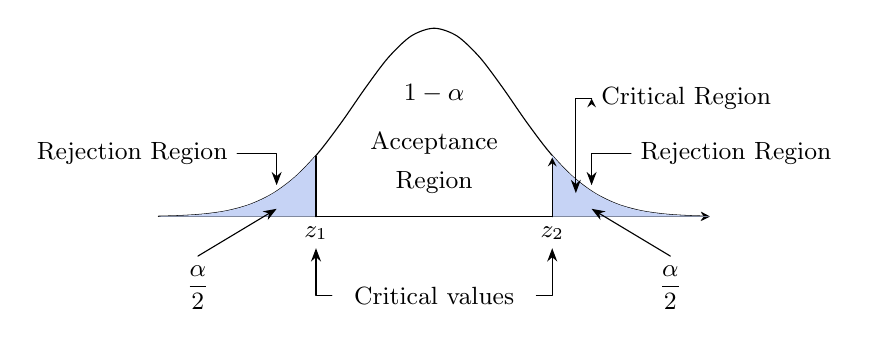
\begin{tikzpicture}[->,>=stealth]
\draw(-3.5,0)--(3.5,0);
\draw[smooth,domain=-3.5:3.5,variable=\x]plot(\x,{6*1/sqrt(2*pi)*exp(-1/2*\x*\x)});
\path[fill=blue!25, smooth, domain=1.5:3.5, variable=\x]plot(\x,{6*1/sqrt(2*pi)*exp(-1/2*\x*\x)})--(3.5,0)--(1.5,0)--(1.5,0.75);
\path[fill=blue!25, smooth, domain=-3.5:-1.5, variable=\x]plot(\x,{6*1/sqrt(2*pi)*exp(-1/2*\x*\x)})--(-1.5,0.75)--(-1.5,0)--(-3.5,0);
\draw(-1.5,0)--(-1.5,0.77)
(1.5,0)--(1.5,0.75);
\draw[-Stealth](-3,-0.5)--(-2,0.1);
\draw[-Stealth](3,-0.5)--(2,0.1);
\draw
(0,1.8)node[below]{$1-\alpha$}
(0,1.2)node[below]{Acceptance}
(0,0.7)node[below]{Region}
(-3,-0.5)node[below]{$\dfrac{\alpha}{2}$}
(3,-0.5)node[below]{$\dfrac{\alpha}{2}$}
(2.5,0.8)node[right]{Rejection Region}
(-2.5,0.8)node[left]{Rejection Region}
(-1.5,0)node[below]{$z_1$}
(1.5,0)node[below]{$z_2$}
(0,-1)node[]{Critical values}
(2,1.5)node[right]{Critical Region};
\draw[-Stealth](-2.5,0.8)--(-2,0.8)--(-2,0.4);
\draw[-Stealth](2.5,0.8)--(2,0.8)--(2,0.4);
\draw[-Stealth](1.3,-1)--(1.5,-1)--(1.5,-0.4);
\draw[-Stealth](-1.3,-1)--(-1.5,-1)--(-1.5,-0.4);
\draw[-Stealth](2,1.5)--(1.8,1.5)--(1.8,0.3);
\end{tikzpicture}
\end{figure}
















\end{enumerate}

$Z_{\alpha/2}$ undirected hypothesis tests, two tailed test $\alpha=5\%$.\\

\textit{Interpretation}: if the statistic $Z$ falls in the critical region we
\textbf{reject} $H_0$ in favour of $H_1$. If it does not, we \textbf{fail to reject}
$H_0$.

Say it that way, and not ``$H_1$ is true'' or ``$H_0$ is true''. A test never establishes
either hypothesis. Rejecting $H_0$ says the data would be unusual if $H_0$ held, which is
evidence against it -- not proof of $H_1$. Failing to reject says only that the data are
consistent with $H_0$; they may be consistent with a great many other values too,
particularly when the sample is small. Absence of evidence is not evidence of absence.\\

We can use the P-value for interpretation given statistic $\alpha=0.025$ \hspace{0.1cm},\hspace{0.2cm}$Z=2.13$


% Daigram 18

\begin{figure}[H]
\centering
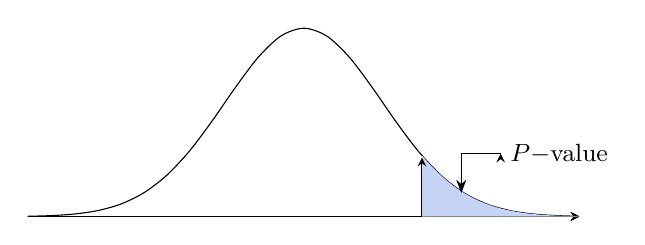
\begin{tikzpicture}[->,>=stealth]
\draw(-3.5,0)--(3.5,0);
\draw[smooth,domain=-3.5:3.5,variable=\x]plot(\x,{6*1/sqrt(2*pi)*exp(-1/2*\x*\x)});
\path[fill=blue!25, smooth, domain=1.5:3.5, variable=\x]plot(\x,{6*1/sqrt(2*pi)*exp(-1/2*\x*\x)})--(3.5,0)--(1.5,0)--(1.5,0.75);
\draw(1.5,0)--(1.5,0.75);
\draw[-Stealth](2.5,0.8)--(2,0.8)--(2,0.3);
\draw(2.5,0.8)node[right]{$P-$value};
\end{tikzpicture}
\end{figure}









\begin{align*}
P(Z>2.13) &=1-P(Z\leq 2.13)=1-0.9834\\
&=0.016
\end{align*}

Because the test is two-tailed, a result this far from the centre is equally surprising in
either direction, so the $P$-value is \emph{both} tails together:
$$P\text{-value} = 2\times P(Z>2.13) = 2\times 0.0166 = 0.033.$$
Since $0.033 < \alpha = 0.05$, we reject $H_0$.

\subsection{The $P$-value}

\begin{definition_}
The \textbf{$P$-value} is the probability of obtaining a result at least as extreme as the
one observed, \emph{assuming the null hypothesis is true}.
\end{definition_}

Every word of that matters, and the last clause most of all. The $P$-value is computed in a
world where $H_0$ holds. It answers ``if nothing were going on, how often would I see
something this striking?'' -- a small value means the data sit awkwardly with $H_0$.

\textbf{The decision rule.} Reject $H_0$ when
$$P\text{-value} < \alpha.$$
Always compare with $\alpha$ itself, never with $\alpha/2$. The halving belongs to the
\emph{critical value} in a two-tailed test, where each tail gets $\alpha/2$. It is applied
once, not twice:
\begin{itemize}
\item \textbf{One-tailed test:} $P = P(Z > z_{\text{obs}})$, the single tail beyond the
statistic.
\item \textbf{Two-tailed test:} $P = 2\times P(Z > |z_{\text{obs}}|)$ -- double it, because
a departure of that size in the opposite direction would have been just as surprising.
\end{itemize}
Doubling the tail \emph{and} halving $\alpha$ would penalise the same two-sidedness twice.

The two approaches always agree. The critical-value method asks whether the statistic is
beyond the boundary; the $P$-value method asks how far beyond it is. The $P$-value carries
more information -- $P = 0.049$ and $P = 0.001$ both ``reject at $5\%$'' while saying very
different things about the strength of the evidence.

\subsubsection{What the $P$-value does not mean}

These misreadings are common enough to be worth stating plainly.

\begin{enumerate}
\item \textbf{It is not the probability that $H_0$ is true.} $H_0$ is either true or it is
not; it has no probability. The $P$-value is a probability about \emph{the data}, computed
assuming $H_0$ -- not a probability about the hypothesis.

\item \textbf{It is not the probability that the result is due to chance.}

\item \textbf{$1-P$ is not the probability that $H_1$ is true.} A $P$-value of $0.03$ does
not make $H_1$ $97\%$ likely.

\item \textbf{A large $P$-value does not show $H_0$ is true.} It shows the data are
consistent with $H_0$. With a small sample, they would be consistent with much else
besides.

\item \textbf{Statistical significance is not practical importance.} A large enough sample
will return a small $P$-value for a difference far too slight to matter. Always ask how
big the effect is, not merely whether it is significant.

\item \textbf{$\alpha=0.05$ is a convention, not a law of nature.} There is nothing
qualitatively different between $P = 0.049$ and $P = 0.051$, and reporting the actual
$P$-value is more honest than reporting only ``significant'' or ``not significant''.
\end{enumerate}







\textbf{Directed Hypothesis Test}\\
One tailed test\\
$H_0:\mu =a\hspace{1cm} H_0:\mu_1=\mu_2$\\
$H_1:\mu >a\hspace{1cm} H_1:\mu_1>\mu_2$\\
$H_1:\mu <a\hspace{1cm} H_1:\mu_1<\mu_2$\\\\




\textbf{Example}\\
Let $n=9$, $\overline{X}=1003$g, $\mu =1 000$g, s.d. = 5g

\begin{enumerate}
\item
\begin{enumerate}
   \item Set up the hypothesis\\
$H_0:$ The machine is correctly set.\\
$H_1:$ The machine is not correctly set.\\\\
or\\
$H_0: \mu =$ 1 000g\\
$H_1: \mu \neq$ 1 000g\\

\item Set up the level of significance $\alpha =5\%$
\item Test statistic\\
This is a small sample size since $n=9<30$ and our S.E $=\dfrac{\sigma}{\sqrt{n}}$.
\begin{align*}
t &=\frac{\overline{X}-\mu}{\dfrac{\sigma}{\sqrt{n}}}=\frac{1003-1000}{5/\sqrt{9}}=\frac{3}{5}\times 3\\\\ \implies\hspace{0.6cm} t&=1.8\\\\
t_{8,0.025}&=2.306\\
\end{align*}
\item Critical region


% Diagram 19


\begin{figure}[H]
\centering
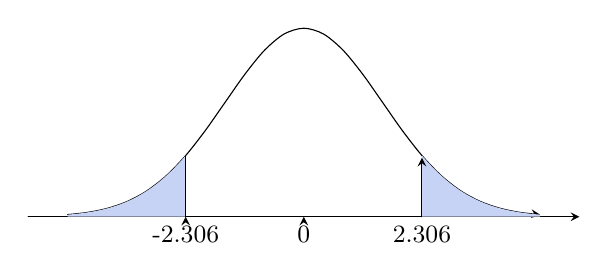
\begin{tikzpicture}[->,>=stealth]
\draw(-3.5,0)--(3.5,0);
\draw[smooth,domain=-3:3,variable=\x]plot(\x,{6*1/sqrt(2*pi)*exp(-1/2*\x*\x)});
\path[fill=blue!25, smooth, domain=1.5:3, variable=\x]plot(\x,{6*1/sqrt(2*pi)*exp(-1/2*\x*\x)})--(3,0)--(1.5,0)--(1.5,0.75);
\path[fill=blue!25, smooth, domain=-3:-1.5, variable=\x]plot(\x,{6*1/sqrt(2*pi)*exp(-1/2*\x*\x)})--(-1.5,0.75)--(-1.5,0)--(-3,0);
\draw(-1.5,0)--(-1.5,0.77)
(1.5,0)--(1.5,0.75);
\draw(0,0)node[below]{0};
\draw(1.5,0)node[below]{2.306}
(-1.5,0)node[below]{-2.306};
\end{tikzpicture}
\end{figure}









\textit{Interpretation}: our statistic $t=1.8$ lies in the acceptance region. That means we accept $H_0$ and reject $H_1$. That is the machine is correctly set up  the level of significance set at $\alpha =5\%$.\\
\end{enumerate}




\pagebreak
\item $H_0: \mu =$ 1 000g\\ $H_1:\mu >$ 1 000g\\\\
$\alpha =5\%$\\\\
$t=1.8$


% Diagram 20


\begin{figure}[H]
\centering
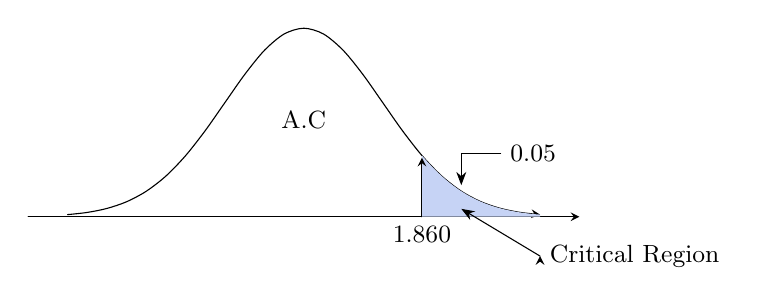
\begin{tikzpicture}[->,>=stealth]
\draw(-3.5,0)--(3.5,0);
\draw[smooth,domain=-3:3,variable=\x]plot(\x,{6*1/sqrt(2*pi)*exp(-1/2*\x*\x)});
\path[fill=blue!25, smooth, domain=1.5:3, variable=\x]plot(\x,{6*1/sqrt(2*pi)*exp(-1/2*\x*\x)})--(3,0)--(1.5,0)--(1.5,0.75);
\draw(1.5,0)--(1.5,0.75);
\draw[-Stealth](2.5,0.8)--(2,0.8)--(2,0.4);
\draw[-Stealth](3,-0.5)--(2,0.1);
\draw(1.5,0)node[below]{1.860}
(0,1)node[above]{A.C}
(2.5,0.8)node[right]{0.05}
(3,-0.5)node[right]{Critical Region};
\end{tikzpicture}
\end{figure}







$t=1.8$ which is less than $t_{8,0.05}=1.860\implies t$ lies in the acceptance region i.e. Accept $H_0$ and reject $H_1$.\\
$\implies$ This machine is correctly set.\\
\end{enumerate}

\textbf{Example}\\
Let $\hspace{0.3cm} \overline{X}=64,\hspace{0.4cm} \mu =60,\hspace{0.4cm} S=6.3,\hspace{0.4cm} n=50$
\begin{enumerate}
\item Set up the hypothesis\\\\
$H_0:\mu =60$\\
$H_1:\mu >60$\\
\item Set up the level of significance at $\alpha=1\%$
\item Test statistic
$$n=50>30\hspace{0.5cm}\implies\hspace{0.5cm}\text{large sample size}$$
\begin{align*}
Z &=\frac{\overline{X}-\mu}{\dfrac{\sigma}{\sqrt{n-1}}}=\frac{64-60}{6.3/\sqrt{49}}=\frac{4\times 7}{6.3}=\frac{28}{6.3}\\\\ \implies\hspace{0.6cm} Z &=4.44\\
\end{align*}
\item Critical region



% Diagram 21

\begin{figure}[H]
\centering
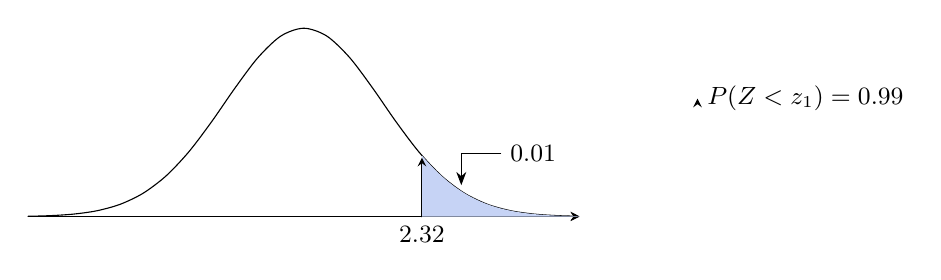
\begin{tikzpicture}[->,>=stealth]
\draw(-3.5,0)--(3.5,0);
\draw[smooth,domain=-3.5:3.5,variable=\x]plot(\x,{6*1/sqrt(2*pi)*exp(-1/2*\x*\x)});
\path[fill=blue!25, smooth, domain=1.5:3.5, variable=\x]plot(\x,{6*1/sqrt(2*pi)*exp(-1/2*\x*\x)})--(3.5,0)--(1.5,0)--(1.5,0.75);
\draw(1.5,0)--(1.5,0.75);
\draw[-Stealth](2.5,0.8)--(2,0.8)--(2,0.4);
\draw(2.5,0.8)node[right]{0.01}
(1.5,0)node[below]{2.32}
(5,1.5)node[right]{$P(Z<z_1)=0.99$};
\end{tikzpicture}
\end{figure}










\end{enumerate}











\subsection{Test for the Variance and Standard Deviation}
When analysing numerical data sometimes you want to draw conclusion about the population variance on s.d. For example if you are told that in a cereal filling process the population s.d. $\sigma$ is equal to 15 grams. To see if the variability of the process has changed you need to test whether the s.d. has changed from the previous specified level of 15 grams.\\ Assume that the data are normally distributed, you use the $\chi^2$ test for the variance $\sigma$ s.d. to test whether the population variance is equal to specified value.\\\\

\textbf{Procedure}
\begin{enumerate}
\item Set up the hypothesis.
\item Set $\alpha$\\\\
$H_0: \sigma^2 = S^2$\\
$H_1: \sigma^2\neq S^2$ for two tailed test.\\\\
$H_1:\sigma^2>S^2$ for the upper one handed test.\\
$H_1: \sigma^2<S^2$ for the lower one handed test.
\item Test statistic $$\chi^2=(n-1)\frac{S^2}{\sigma^2}$$
\item Critical Region

% Diagram 22


\begin{figure}[H]
\centering
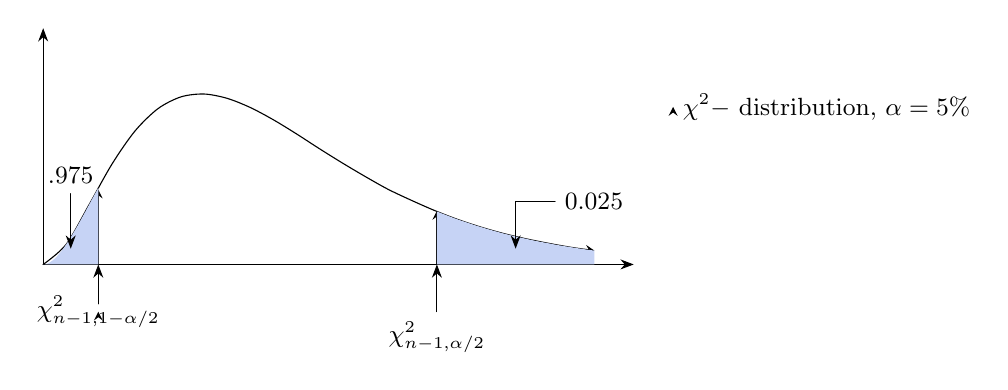
\begin{tikzpicture}[->,>=stealth]
\draw[-Stealth](0,0)--(7.5,0);
\draw[-Stealth](0,0)--(0,3);
\draw[smooth,domain=0:14,scale=0.5,variable=\x]plot(\x,{8*\x*\x*exp(-1/2*\x)/4});
\draw(5,0)--(5,0.68);
\draw(8,2)node[right]{$\chi^2-$ distribution, $\alpha = 5\%$};
\draw(0.7,0)--(0.7,0.95);
\path[fill=blue!25, smooth, domain=10:14,scale=0.5,variable=\x]plot(\x,{8*\x*\x*exp(-1/2*\x)/4})--(14,0.18)--(14,0)--(10,0)--(10,0.68)--cycle;
\path[fill=blue!25, smooth, domain=0:1.4,scale=0.5,variable=\x]plot(\x,{8*\x*\x*exp(-1/2*\x)/4})--(1.4,0.95)--(1.4,0)--(0,0)--cycle;
\draw[-Stealth](0.35,0.9)--(0.35,0.2);
\draw[-Stealth](6.5,0.8)--(6,0.8)--(6,0.2);
\draw[-Stealth](0.7,-0.5)--(0.7,0);
\draw[-Stealth](5,-0.6)--(5,0);
\draw(6.5,0.8)node[right]{0.025}
(0.35,0.9)node[above]{.975}
(5,-0.6)node[below]{$\chi^2_{n-1,\alpha /2}$}
(0.7,-0.6)node[]{$\chi^2_{n-1,1-\alpha /2}$};
\end{tikzpicture}
\end{figure}





The formula for the hypothesis can easily be converted to form an interval estimate for the variance 
$$\frac{(n-1)S^2}{\chi^2_{\alpha/2,n-1}}\leq \sigma^2\leq \frac{(n-1)S^2}{\chi^2_{1-\alpha/2,n-1}}$$\\



Confidence interval for the ratio of variances $$\dfrac{S_1^2}{S^2_2}\,\cdot\,\dfrac{1}{F_{\frac{\alpha}{2},n_1-1,n_2-1}}\leq \dfrac{\sigma^2_1}{\sigma_2^2}\leq \dfrac{S_1^2}{S_2^2}\,\cdot\, F_{\frac{\alpha}{2},n_2-1,n_1-1}$$
\end{enumerate}






\pagebreak
\textbf{Chi-Square Tests}\\

$\chi^2$ distribution
\begin{enumerate}
\item[$\bullet$] It has only one parameter, called the degrees of freedom (df)
\item[$\bullet$] The random variable $\chi^2$ assumes non negative values only.
\item[$\bullet$] The shape of a Chi-square distribution curve is skewed to the right for small df and becomes symmetric for large df.
\item[$\bullet$] The entire $\chi^2$-distribution curve lies to the right of the vertical axis.
\end{enumerate}






\textbf{Example}\\
Find the value of $\chi^2$ for 7 degrees of freedom and an area of 0.10 in the right tail of the Chi square distribution curve.\\

\textbf{Solution}\\
From the table, locate 7 in the column for df and 0.10 in top row


\begin{figure}[H]
\centering
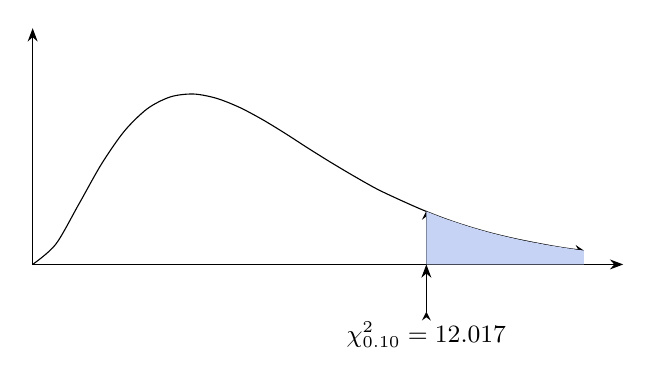
\begin{tikzpicture}[->,>=stealth]
\draw[-Stealth](0,0)--(7.5,0);
\draw[-Stealth](0,0)--(0,3);
\draw[smooth,domain=0:14,scale=0.5,variable=\x]plot(\x,{8*\x*\x*exp(-1/2*\x)/4});
\draw(5,0)--(5,0.68);
\path[fill=blue!25, smooth, domain=10:14,scale=0.5,variable=\x]plot(\x,{8*\x*\x*exp(-1/2*\x)/4})--(14,0.18)--(14,0)--(10,0)--(10,0.68)--cycle;
\draw[-Stealth](5,-0.6)--(5,0);
\draw(5,-0.6)node[below]{$\chi^2_{0.10}=12.017$};
\end{tikzpicture}
\end{figure}





\textbf{Example}\\
Find the value of $\chi^2$ for 12 degrees of freedom and an area of 0.5 in the left tail of the Chi-square distribution curve.\\

\textbf{Solution}\\
Area in the right tail = $1 - $ Area in the left $= 1 - 0.05=0.95$\\

Next, we locate 12 in the column for df and 0.950 in the top row \hspace{0.2cm}$\chi^2_{.950,12}=5.226$\\\\











\textbf{Example}\\
A dairy processing company claims that the variance of the amount of fat in the whole milk processed by the company is no more than 0.25. You suspect this is wrong and find that a random sample of 41 milk contains has a variance of 0.27. At $\alpha =5\%$ is this enough evidence to reject the company's claims? Assume the population is normally distributed.\\\\

\textbf{Solution}
\begin{enumerate}
\item Set up the hypothesis\\\\
$H_0:\sigma^2 \leq 0.25$\\ $H_1:\sigma^2>0.25$\\
\item Set $\alpha =5\%$ level of significance.
\item Test Statistic\\
We have $n=41,\hspace{0.4cm} \sigma^2=0.25,\hspace{0.4cm} S^2=0.27,\hspace{0.4cm}$ df = 40
\begin{align*}
\chi^2 &=(n-1)\frac{S^2}{\sigma^2}=\frac{(41-1)(0.27)^2}{(0.25)^2}\\\\ \implies\hspace{0.6cm} \chi^2 &\approx 43.2\\
\end{align*}



\item Critical Region


% Diagram 23

\begin{figure}[H]
\centering
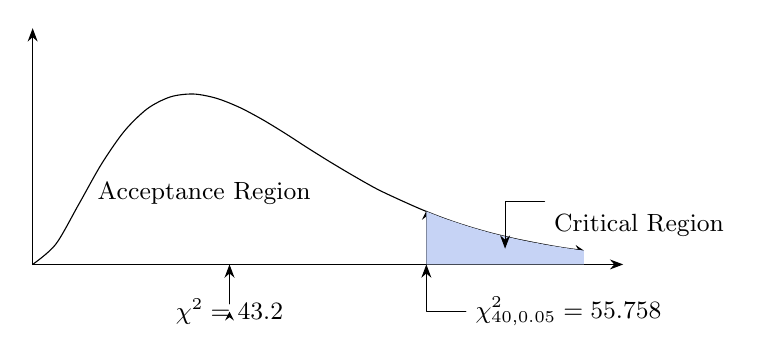
\begin{tikzpicture}[->,>=stealth]
\draw[-Stealth](0,0)--(7.5,0);
\draw[-Stealth](0,0)--(0,3);
\draw[smooth,domain=0:14,scale=0.5,variable=\x]plot(\x,{8*\x*\x*exp(-1/2*\x)/4});
\draw(5,0)--(5,0.68);
\path[fill=blue!25, smooth, domain=10:14,scale=0.5,variable=\x]plot(\x,{8*\x*\x*exp(-1/2*\x)/4})--(14,0.18)--(14,0)--(10,0)--(10,0.68)--cycle;
\draw[-Stealth](6.5,0.8)--(6,0.8)--(6,0.2);
\draw[-Stealth](2.5,-0.5)--(2.5,0);
\draw[-Stealth](5.5,-0.6)--(5,-0.6)--(5,0);
\draw(6.5,0.5)node[right]{Critical Region}
(0.7,0.9)node[right]{Acceptance Region}
(5.5,-0.6)node[right]{$\chi^2_{40,0.05}=55.758$}
(2.5,-0.6)node[]{$\chi^2=43.2$};
\end{tikzpicture}
\end{figure}









Interpretation: Our statistic $\chi^2=43.2$ is less than the critical value, $\chi^2_{0.05}=55.758$. That is our statistic lies in the Acceptance region.\\\\ We accept $H_0$ and reject $H_1$, that is the company's claims is true.\\
\end{enumerate}

\textbf{Example}\\
A cereal process is set at the s.d. of 15 grams. A sample of 25 packets has a s.d. of 17.7 grams, is there enough evidence that the process has changed?\\


\subsection{Type I and Type II Errors}
When we test a null hypothesis by applying a significant test to a sample, we can never be certain that our conclusion is correct.\\ All we know is that our decision is probably correct.\\ That is when we reject $H_0$, it is because our statistic lies in the CR and this event is unlikely if the null hypothesis is true we can make two types of errors.\\\\
Type I error: The null hypothesis is rejected when in fact it is true $(\alpha)$.\\\\
Type II error: The null hypothesis is retained when in fact it is false $(\beta)$.\\\\
The probability of type II error can not be generally calculated because it depends  on the population mean which is unknown. $\beta$ can be computed if $\mu$, $\sigma^2$, $n$ are given.\\ The power of a hypothesis test is simply $1-\beta$. And this is basically (power of a test) is  the probability that we make the right decision when the null hypothesis is not correct (we correctly reject $H_0$).\\\\

\textbf{Example}\\\\
$H_0: \mu \geq 30$\\
$H_1:\mu <30$\\\\

we are given $\sigma^2=10 000$, $n=100$ $$\sigma^2_{\overline{X}}=\frac{\sigma^2}{n}=\frac{10 000}{100}$$\\ $$\implies\hspace{0.5cm}\sigma_{\overline{X}}=\frac{\sigma}{\sqrt{n}}=10$$
What we want is to calculate $\beta$ conditional on particular value of $\mu$. Let $\mu =26$ and $\alpha =5\%$\\\\
We know:
\begin{enumerate}
\item This is a one tailed test (left).
\item We will fail to reject $H_0$ if we get a statistic greater than $Z_{0.05}$.
\item C.V is $-1.64$. This corresponds to $\overline{X}$ value.\\
\end{enumerate}

$$P(Z-\text{statistic} \geq -1.64)=P\Big(\overline{X}>\overline{X}_i|\mu =30,\hspace{0.2cm} \sigma_{\overline{X}}\Big)=0.95$$

\begin{align*}
Z_c &\frac{\overline{X}_c-\mu}{\sigma_{\overline{X}}}\hspace{0.6cm}\implies\hspace{0.5cm} -1.64=\frac{\overline{X}_c-30}{10}\\\\
\implies\hspace{0.6cm}\overline{X}_c &=13.6\\
\end{align*}

So we will incorrectly fail to reject $H_0$ as long as a draw of sample mean is greater than 13.6.\\\\
So we calculate the probability of drawing a sample mean greater than 13.6, $\mu =26$, $\sigma_{\overline{X}}=10$\\\\ Probability of $\beta$ is
\begin{align*}
P\Big(\overline{X}>13.6|\mu =26,\hspace{0.2cm}\sigma_{\overline{X}=10}\Big) &=P\Bigg(Z>\frac{13.6-26}{10}\Bigg)\\\\
&=P(Z>-1.26)\\
&=0.8925=\beta\\
\end{align*}
and the power of the test is 0.1075, $(1-\beta)=$ power of the test.\\\\










\subsection{Test of Independence and Goodness of Fit Test}
The $\chi^2$ test is used to determine whether there is a significant difference between the observed and expected frequencies in one or more categories.\\\\
Do the number of individuals or objects that fall in each category differ significantly from the number you would expect? Is the difference merely sampling error, or is it real? That is what the test decides.\\\\
\textbf{$\chi^2$ Test}
\begin{enumerate}
\item Quantitative data
\item One or more categories
\item Independent observations
\item Enough sample size (at least 10)
\item Simple random sampling
\item Data frequencies\\
\end{enumerate}
% The exponent here read (O-E)^1, and the formula was then restated correctly
% just below with a lower-case e. Squared, and the notation made consistent.
$$\text{Test statistic}\hspace{0.4cm}
\chi^2=\sum \frac{(O-E)^2}{E}$$
Where:\\\\
$O-$ the observed frequency in a category\\
$E-$ the expected frequency in that category, if $H_0$ were true\\
$\chi^2-$ the test statistic.\\

The differences are \emph{squared}, so that shortfalls and excesses both count against
$H_0$ rather than cancelling, and each is divided by $E$ so that a discrepancy is judged
against the size of the category it occurs in -- being 10 out on an expected 20 matters far
more than being 10 out on an expected 2000.

\textbf{Degrees of freedom.} These are not $n-1$, where $n$ is the sample size. They count
the categories, not the observations:
\begin{itemize}
\item \textbf{Goodness of fit:} $\text{df} = k-1-m$, where $k$ is the number of categories
and $m$ the number of parameters estimated from the data. The $-1$ appears because the
expected frequencies are constrained to the same total as the observed ones, so once $k-1$
of them are fixed the last is determined.
\item \textbf{Test of independence:} $\text{df} = (r-1)(c-1)$ for an $r\times c$
contingency table, since the row and column totals are fixed.
\end{itemize}

The $\chi^2$ - test should be used when the sampling distribution $\chi^2\approx \chi^2_c$ distribution.\\

The conditions for these are:
\begin{enumerate}
\item The total frequencies is not less than 50.
\item The expected class frequencies are not less than 5.\\
\end{enumerate}

If the second condition is not met it can be improved where $v=1$ by making an adjustment known as YATES correction which involves reducing value of $|O-e|$ by 1/2.\\\\




\textbf{Example}\\
Four coins where tossed 160 times , the results are given below showing the number of heads is this evidence that this coin is balanced.

\begin{table}[H]
\centering
\begin{tabular}{c|ccccc}
number of heads & 0& 1& 2& 3&4\\
\hline $O$ & 15& 46& 54& 35& 10\\
\end{tabular}
\end{table} 




\vspace{3cm}
\textbf{Solution}
\begin{enumerate}
\item Set up the hypothesis\\\\
$H_0: P=1/2$ vs $H_1:P>1/2$
\item Set $\alpha =0.05$
\item Test statistic:\hspace{0.3cm}
$\displaystyle{\chi^2=\frac{\sum (O-e)^2}{e}}$


\begin{table}[H]
\centering
\begin{tabular}{|c|c|c|c|c|}
\hline No of Heads & $O$ &$e$& $(O-e)^2$ &$\dfrac{(O-e)^2}{e}$\\
\hline 0&15& $160\times P(0)=10$ &&\\
1&46&$160\times P(1)=40$&&\\
2&54&= 60&&\\
3&35&= 40&&\\
4&10&= 10&&\\
\hline &&&&4.625\\
\hline
\end{tabular}
\end{table}

\begin{align*}
P(x) &=
\begin{pmatrix}
n\\4\\
\end{pmatrix}
P^x(1-P)^{n-x}\\\\
e(0)=160\times P(0) &=160\times
\begin{pmatrix}
4\\0\\
\end{pmatrix}
\Big(\frac{1}{2}\Big)^0\Big(\frac{1}{2}\Big)^4=160\times \frac{1}{16}=10\\
\end{align*}
Our statistic is $\chi^2=4.625$\\


\item Critical Region


% Diagram 25


\begin{figure}[H]
\centering
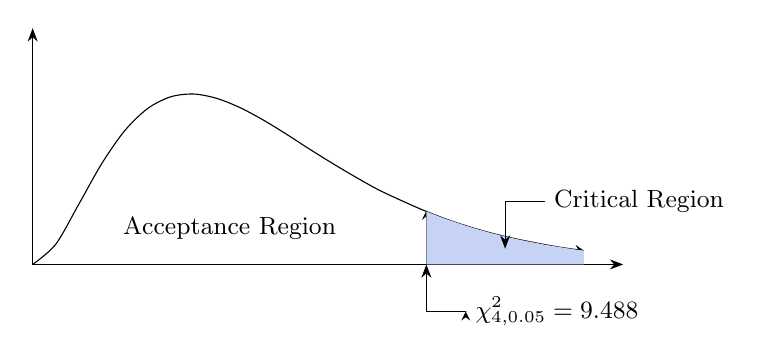
\begin{tikzpicture}[->,>=stealth]
\draw[-Stealth](0,0)--(7.5,0);
\draw[-Stealth](0,0)--(0,3);
\draw[smooth,domain=0:14,scale=0.5,variable=\x]plot(\x,{8*\x*\x*exp(-1/2*\x)/4});
\draw(5,0)--(5,0.68);
\path[fill=blue!25, smooth, domain=10:14,scale=0.5,variable=\x]plot(\x,{8*\x*\x*exp(-1/2*\x)/4})--(14,0.18)--(14,0)--(10,0)--(10,0.68)--cycle;
\draw[-Stealth](6.5,0.8)--(6,0.8)--(6,0.2);
\draw[-Stealth](5.5,-0.6)--(5,-0.6)--(5,0);
\draw(6.5,0.8)node[right]{Critical Region}
(2.5,0.2)node[above]{Acceptance Region}
(5.5,-0.6)node[right]{$\chi^2_{4,0.05}=9.488$};
\end{tikzpicture}
\end{figure}


















Interpretation: Our statistic $\chi^2=4.625$ lies in the acceptance region.\\\\
We accept $H_0$ and reject $H_1$. That is the distribution follows a Binomial with $P=1/2$, $n=4$.\\ $\therefore$ The coin is balanced, P-value is 0.075\\\\
Since the P-value is greater than 0.05 $\implies$ Accept $H_0$ and reject $H_1$.\\
\end{enumerate}



\textbf{Example}\\
On a national bases the success rate for the people taking the driving test for the first time is $40\%$. A driving instructors records show that for the 50 pupils of his who took the test for the first time last year 25 passed.\\ Does his success rate differ from the national success rate?\\

\textbf{Solution}
\begin{enumerate}
\item Set up the hypothesis\\
$H_0: P=0.40$\\
$H_1: P\neq 0.40$

\item Set up level of significance $\alpha =0.05$
\item Test statistic \hspace{0.2cm}$\displaystyle{\chi^2=\frac{\sum (O-e)^2}{e}}$

\begin{table}[H]
\centering
\begin{tabular}{|c|c|c|c|c|c|}
\hline & $O$ & $e$ & $|O-e|$ & $|O-e|-\frac{1}{2}$ & $(|O-e|-1/2)^2$\\
\hline Passed & 25 &20 & 5 & 4.5 & 1.0015\\
fail & 25 & 30 &&&\\
\hline &&&&&1.6875\\
\hline
\end{tabular}
\end{table}

\item Critical Region


% Diagram 26


\begin{figure}[H]
\centering
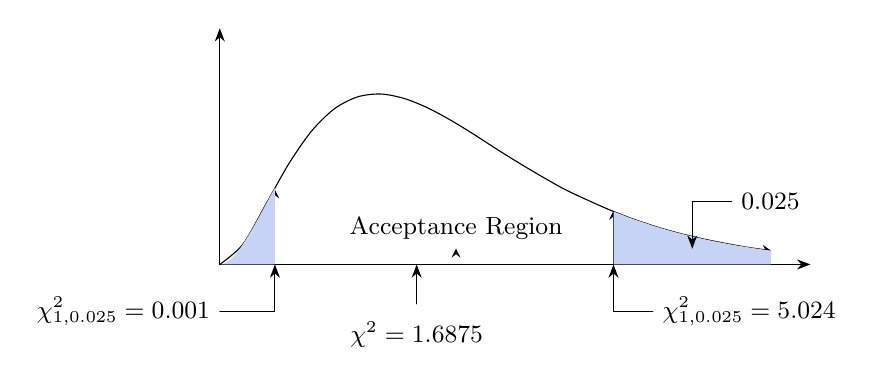
\begin{tikzpicture}[->,>=stealth]
\draw[-Stealth](0,0)--(7.5,0);
\draw[-Stealth](0,0)--(0,3);
\draw[smooth,domain=0:14,scale=0.5,variable=\x]plot(\x,{8*\x*\x*exp(-1/2*\x)/4});
\draw(5,0)--(5,0.68);
\draw(0.7,0)--(0.7,0.95);
\path[fill=blue!25, smooth, domain=10:14,scale=0.5,variable=\x]plot(\x,{8*\x*\x*exp(-1/2*\x)/4})--(14,0.18)--(14,0)--(10,0)--(10,0.68)--cycle;
\path[fill=blue!25, smooth, domain=0:1.4,scale=0.5,variable=\x]plot(\x,{8*\x*\x*exp(-1/2*\x)/4})--(1.4,0.95)--(1.4,0)--(0,0)--cycle;
\draw[-Stealth](6.5,0.8)--(6,0.8)--(6,0.2);
\draw[-Stealth](2.5,-0.5)--(2.5,0);
\draw[-Stealth](5.5,-0.6)--(5,-0.6)--(5,0);
\draw[-Stealth](0,-0.6)--(0.7,-0.6)--(0.7,0);
\draw(6.5,0.8)node[right]{0.025}
(5.5,-0.6)node[right]{$\chi^2_{1,0.025}=5.024$}
(2.5,-0.6)node[below]{$\chi^2=1.6875$}
(0,-0.6)node[left]{$\chi^2_{1,0.025}=0.001$}
(3,0.2)node[above]{Acceptance Region};
\end{tikzpicture}
\end{figure}









P-value is 0.975\\
Since P -value is greater than 0.025 $\implies$ We accept $H_0$ and reject $H_1$.\\
\end{enumerate}
% THE END






\pagebreak
\subsection{Practice problems}

\begin{problem}{Exercises on Hypothesis Testing}
A machine should be set to produce bags of sugar whose weights are normally distributed
with mean $1000$\,g and standard deviation $5$\,g. To check the setting, a sample of nine
bags is taken and the mean is found to be $1003$\,g.
\begin{enumerate}
\item[(a).] Is the machine correctly set? (Assume the standard deviation cannot change.)
\item[(b).] Is the machine set too high?
\end{enumerate}
\end{problem}

\begin{solution}
Note first that $\sigma = 5$ is \emph{known} and cannot change, so the test statistic is
$Z$ -- not $t$, despite $n = 9$ being small. The population is stated to be normal, which
is what a small sample requires.
$$Z=\frac{\overline{X}-\mu_0}{\sigma/\sqrt{n}}
 =\frac{1003-1000}{5/\sqrt{9}}=\frac{3}{5/3}=1.80.$$

\textbf{(a).} ``Correctly set'' means neither too high nor too low, so this is
\textbf{two-tailed}:
$$H_0:\mu=1000 \qquad\text{against}\qquad H_1:\mu\neq 1000.$$
At $\alpha=0.05$ the critical values are $\pm 1.96$. Since $|1.80|<1.96$ we
\textbf{fail to reject} $H_0$. Equivalently, the $P$-value is
$2\times P(Z>1.80)=0.072$, which exceeds $0.05$. There is no evidence that the machine is
incorrectly set.

\textbf{(b).} ``Set too high'' names a direction, so this is \textbf{one-tailed}:
$$H_0:\mu=1000 \qquad\text{against}\qquad H_1:\mu>1000.$$
The critical value is now $Z_{0.05}=1.645$, and $1.80>1.645$, so we \textbf{reject} $H_0$.
The $P$-value is $P(Z>1.80)=0.036$, below $0.05$.

\medskip
The two parts use the \emph{same data} and reach \emph{opposite conclusions}, and that is
the point of the question. A one-tailed test puts the whole of $\alpha$ into one tail, so
it is more willing to reject in that direction -- $1.645$ against $1.96$. The price is that
it cannot detect a departure the other way at all: had the mean come out at $997$, part (b)
would have found nothing whatever.

This is why the alternative hypothesis must be chosen \emph{before} seeing the data. Picking
the one-tailed version after noticing the mean came out high is not a stronger test; it is
a way of manufacturing significance.
\end{solution}

\begin{problem}{Exercises on Hypothesis Testing}
The times taken by a salesman to travel between two shops on 50 occasions averaged 64
minutes with a standard deviation of $6.3$ minutes. He claims that this is evidence that the
journey takes longer since he changed to a smaller car, as before he averaged 60 minutes.
Do you agree with the salesman?
\end{problem}

\begin{solution}
Here $\sigma$ is unknown, but $n=50$ is large, so $Z$ serves. Testing
$H_0:\mu=60$ against $H_1:\mu>60$:
$$Z=\frac{64-60}{6.3/\sqrt{50}}=\frac{4}{0.891}=4.49.$$
This is far beyond $1.645$; the $P$-value is about $0.0000036$. The journey time has
certainly increased.

\medskip
\textbf{But that is not what the salesman claimed.} He claimed the journey takes longer
\emph{because he changed to a smaller car}. The test establishes that the times are longer;
it says nothing whatever about the cause. These are observational data, not an experiment:
the car was not assigned at random, and nothing was held constant. Traffic may have grown
heavier, the route may have changed, roadworks may have appeared, he may be older or busier.

So: agree that the journey now takes significantly longer. Do not agree that the car is the
reason. A statistical test can tell you that something changed; only a controlled comparison
can tell you what changed it.
\end{solution}

\begin{problem}{Exercises on Hypothesis Testing}
A manufacturer claims that his light bulbs have an average lifetime of $1500$ hours. A
purchaser checks this and finds that six bulbs last
$$1472,\quad 1486,\quad 1401,\quad 1350,\quad 1610,\quad 1590 \text{ hours}.$$
Does this evidence support the manufacturer's claim?
\end{problem}

\begin{solution}
With $n=6$ and $\sigma$ unknown, this calls for $t$ with $n-1=5$ degrees of freedom.
$$\overline{X}=\frac{8909}{6}=1484.83, \qquad \widehat{S}=102.08.$$
Testing $H_0:\mu=1500$ against $H_1:\mu\neq 1500$:
$$t=\frac{1484.83-1500}{102.08/\sqrt{6}}=\frac{-15.17}{41.67}=-0.364.$$
The critical value is $t_{5,\,0.025}=2.571$, and $|-0.364|$ is nowhere near it. The
$P$-value is $0.73$. We fail to reject $H_0$: the evidence is consistent with the claim.

\medskip
Consider \emph{why} it is consistent. The sample mean is 15 hours below the claim, but the
bulbs themselves range from 1350 to 1610 -- a standard deviation of over 100 hours. Against
that much variation, and with only six observations, a shortfall of 15 hours is nothing.

Note what this does \emph{not} say. It does not show the claim is true. With six bulbs the
test would also have failed to detect a genuine mean of 1450, or 1550. The purchaser has not
confirmed the manufacturer's figure; they have merely failed to contradict it, which is a
much weaker thing and would take a far larger sample to improve.
\end{solution}

\begin{problem}{Exercises on Hypothesis Testing}
A firm employs 300 women and 100 men. The mean number of days absent last year for the women
was $5.3$ with a standard deviation of $2.2$; for the men the figures were $6.2$ and $2.9$.
Is the difference between the means significant?
\end{problem}

\begin{solution}
Two independent samples, both large, so $Z$ applies. Testing
$H_0:\mu_M=\mu_W$ against $H_1:\mu_M\neq\mu_W$, the standard error of the difference is
$$SE=\sqrt{\frac{s_M^2}{n_M}+\frac{s_W^2}{n_W}}
=\sqrt{\frac{2.9^2}{100}+\frac{2.2^2}{300}}=\sqrt{0.0841+0.0161}=0.317,$$
and
$$Z=\frac{6.2-5.3}{0.317}=2.84.$$
Since $|2.84|>1.96$ we reject $H_0$ at the $5\%$ level; the $P$-value is $0.0045$. The
difference is statistically significant.

\medskip
Whether it \emph{matters} is a separate question. The difference is $0.9$ of a day per year.
Whether that is worth acting on is a judgement about the firm, not a statistical one -- and
with 400 employees the study is large enough to detect differences far too small to be of
any practical use. Significance and importance are not the same thing.
\end{solution}

\begin{problem}{Exercises on Hypothesis Testing}
A market gardener tests a new pesticide, which the manufacturers claim increases yields, by
applying it to one of his two orchards. The treated orchard contains twenty trees, with mean
yield $98$\,kg and standard deviation $10$\,kg. The untreated orchard contains fifteen trees,
with corresponding values $94$\,kg and $8$\,kg. Test whether these results are consistent
with the yields being drawn from the same population.
\end{problem}

\begin{solution}
Both samples are small and $\sigma$ is unknown, so this is a pooled two-sample $t$-test. The
variances are close enough to pool -- $\tfrac{100}{64}=1.56$, comfortably inside the
$\tfrac12$ to $2$ guideline:
$$S_p^2=\frac{(n_1-1)\widehat{S}_1^2+(n_2-1)\widehat{S}_2^2}{n_1+n_2-2}
=\frac{19(100)+14(64)}{33}=\frac{2796}{33}=84.73, \qquad S_p=9.20.$$
$$SE=S_p\sqrt{\frac{1}{20}+\frac{1}{15}}=9.20\times 0.342=3.14,
\qquad t=\frac{98-94}{3.14}=1.27$$
with $n_1+n_2-2=33$ degrees of freedom. The critical value is $t_{33,\,0.025}=2.035$, and
the $P$-value is $0.21$. We fail to reject $H_0$: the results are consistent with both
orchards being drawn from the same population.

\medskip
Two remarks. First, the treated orchard did yield $4$\,kg more on average -- but with trees
varying by $8$ to $10$\,kg about their own means, a gap that size is unremarkable. The
pesticide has not been shown to work.

Second, and more seriously, \textbf{the experiment cannot answer the question even in
principle}. One whole orchard was treated and the other was not, so ``pesticide'' is
completely confounded with ``orchard'' -- with its soil, drainage, aspect, age of trees and
everything else. Had the difference been significant, we still could not have attributed it
to the pesticide. A sound design would assign treatment to \emph{individual trees at random
within both orchards}, which is exactly what the next chapter's randomised block design
sets out to do.
\end{solution}

\section{Analysis of Variance}
\subsection{Contingency Table }
A contingency table is used when results are put in cells as: Rows and Columns.

\begin{table}[H]
\centering
\begin{tabular}{|c|c|c}
\hline a&b& $R_1$\\
c&d&$R_2$\\
\hline $C_1$& $C_2$ &$g$
\end{tabular}
$\hspace{0.5cm}$ This is a $2\times 2$ contingency table df $=(r-1)(c-1)$\\
\end{table}

$\therefore$ a $2\times 2$ contingency table has 1 df.\\

\begin{table}[H]
\centering
\begin{tabular}{|c|c|}
\hline $c_1R_1/g$ & $c_1R_2/g$\\
\hline $c_1R_2/g$ & $c_2R_2/g$\\
\hline
\end{tabular}
$\hspace{1cm}$ Expected values\\
\end{table}



The table below shows the result of prevention of a disease by vaccination
\begin{table}[H]
\centering
\begin{tabular}{c|c|c|c}
\cline{2-3}
 & Attacked & Not Attacked &\\
\hline Vaccinated & 20 & 50 & 70\\
% &&&\\
Not Vaccinated & 15 & 15 & 30\\
\hline & 35 & 65 & 100\\
\end{tabular}
\end{table}

Test the hypothesis that vaccination is effective against the disease.\\\\


\textbf{Solution}


\begin{table}[H]
Expected\hspace{1cm}
\begin{tabular}{|c|c|}
\hline 
$\dfrac{35\times 70}{100}$ & $\dfrac{65\times 70}{100}$\\
\hline 
$\dfrac{35\times 30}{100}$ & $\dfrac{65\times 30}{100}$\\
\hline
\end{tabular}
\end{table}



\vspace{1cm}
The $\chi^2$ distribution depends on the df, therefore we write $\chi^2_v$. That is $v=n-1$ is called degree of freedom is the number of expected frequencies which can be varied independently $2\times 2$ contingency table has $v=1$ df because a column loses 1 df and the rows lose 1 df to give $v=(2-1)(2-1)$. The table below shows the seven results for a random sample of 4146 people on the type of house and compound.


\begin{table}[H]
\centering
\begin{tabular}{c|ccc|c}
& Detail & Data & Flats & Total\\
\hline Chelstone & 95 & 297 & 362 & 754\\
Northmead & 175 & 417 & 362 & 954\\
Kabwata & 703 & 994 & 861 & 2556\\
\hline Total & 973 & 1708 &  1585 & 4266\\
\end{tabular}
\end{table}

Does the type of housing vary between the compounds.\\\\\\


$H_0:$ The type of housing and compound are independent.\\
$H_1:$ The type of housing and compound are dependent.\\
$$\chi^2=\frac{\sum (O-e)^2}{e}=33.48$$ $$\chi^2_{4,0.05}=$$\\

\textbf{F Value = 0.01}\\
The P-value of 0.01 is less than our level of significance = 0.05 $\implies$ reject $H_0$ and accept $H_1$.


% Diagram 27

\begin{figure}[H]
\centering
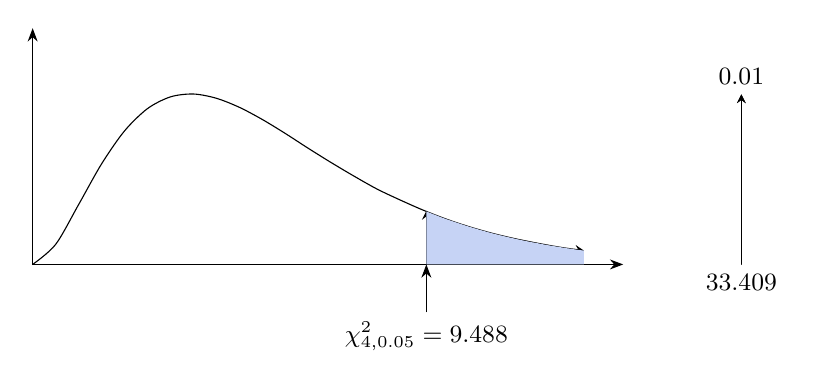
\begin{tikzpicture}[->,>=stealth]
\draw[-Stealth](0,0)--(7.5,0);
\draw[-Stealth](0,0)--(0,3);
\draw[smooth,domain=0:14,scale=0.5,variable=\x]plot(\x,{8*\x*\x*exp(-1/2*\x)/4});
\draw(5,0)--(5,0.68);
\path[fill=blue!25, smooth, domain=10:14,scale=0.5,variable=\x]plot(\x,{8*\x*\x*exp(-1/2*\x)/4})--(14,0.18)--(14,0)--(10,0)--(10,0.68)--cycle;
\draw[-Stealth](5,-0.6)--(5,0);
\draw
(5,-0.6)node[below]{$\chi^2_{4,0.05}=9.488$}
(9,0)node[below]{33.409}
(9,2.16)node[above]{0.01};
\draw(9,0)--(9,2.16);
\end{tikzpicture}
\end{figure}


















Analysis of variance is used to check the variability of more than two samples since we can not use the four\\\\

$H_0:\mu_1=\mu_2$\\
$H_1:\mu_1\neq \mu_2$\\

$\mu_1>\mu_2$\\ $\mu_1<\mu_2$\\\\

$(*)$ One way ANOVA is used for either column or row\\ $(*)$ Two way ANOVA is used fro resting both rows and columns.\\\\
$H_0:$ There is no difference between fertilizers\\ $\mu_1=\mu_2=\mu_3=\mu_4$, $(\mu_i=\mu)\hspace{0.1cm}i=1,2,3,4$\\\\
$H_1:$ At least two fertilizers are different $(\mu_i \neq \mu)$\\\\

\textbf{Example}

\begin{table}[H]
\begin{tabular}{ccc}
$F_1$ & $F_2$ & $F_3$\\
\hline 3 & 2 & 5\\
2 & 4 & 2\\
1 & 3 & 4\\
2 & 5 & 1\\
\hline
\end{tabular}
\end{table}

\begin{align*}
T(\text{sum of all n observations}) & = T =\sum x_{ij}\\\\
SS_T  = \text{Total sum of squares} &= SS_T = \sum x^2_{ij}-\frac{T^2}{n}\\\\
% This read T^2/n_j, using the GRAND total in every term. It must be the total
% of each group, T_j, or the quantity is not a between-groups sum of squares at
% all - on a worked check it came out 46896 against a true 55.6.
SS_B = \text{Between samples sum of squares} & = SS_B = \sum_{j=1}^{k}\frac{T_j^2}{n_j}-\frac{T^2}{n}\\\
SS_W = \text{Within sample sum of squares} &= SS_W =SS_T - SS_B\\\\
MS_{\varepsilon} & =\text{mean square error} = \frac{SS_W}{n-k}\\
\end{align*}





\begin{table}[H]
\centering
ANOVA TABLE (one way variation)\\
\begin{tabular}{|c|c|c|c|c|}
\hline
Squares of Variance & SS & df & MS & F-statistics\\
\hline
Between Sample & $SS_B$ & $v_1=k-1$ & $\dfrac{SS_B}{k-1}=MS_B$ & $F-\dfrac{MS_B}{MS_{\varepsilon}}$\\
Within Sample & $SS_{\varepsilon}$ & $v_2=n-k$ & $\dfrac{SS_{\varepsilon}}{n-k}=MS_{\varepsilon}$ &\\
\hline
Total & $SS_T$ & $n-1$ &&\\
\hline
\end{tabular}
\end{table}



\hspace{1cm}


% Diagram 28


\begin{figure}[H]
\centering
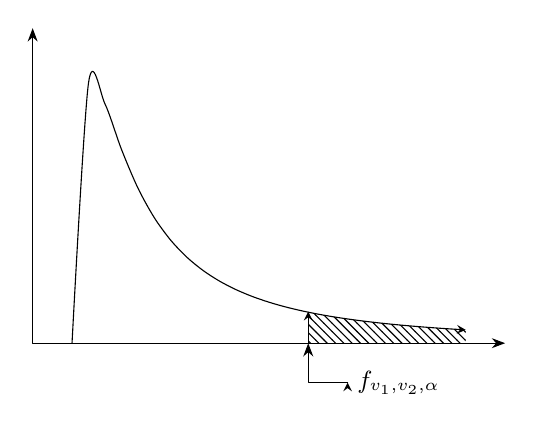
\begin{tikzpicture}[->,>=stealth]
\draw[-Stealth](-0.5,0)--(5.5,0);
\draw[-Stealth](-0.5,0)--(-0.5,4);
\draw[smooth, domain=0:10, scale=0.5,variable=\x]plot(\x,{45*\x/((1 + \x)*(1+\x)*(1+\x))});
\draw(3,0)--(3,0.4);
\path[pattern = north west lines, smooth, domain=6:10, scale=0.5,variable=\x]plot(\x,{45*\x/((1 + \x)*(1+\x)*(1+\x))})--(10,0.17)--(10,0)--(6,0)--(6,0.4)--cycle;
\draw[-Stealth](3.5,-0.5)--(3,-0.5)--(3,0);
\draw(3.5,-0.5)node[right]{$f_{v_1,v_2,\alpha}$};
\end{tikzpicture}
\end{figure}









\textbf{Assumptions Made In Analysis Of Variance}
\begin{enumerate}
\item The $k$ parent population from which the samples are drawn are normally distributed with respective means $\mu_1, \mu_2,....... , \mu_n$.
\item The samples drawn are randomly and independently.
\item The population have equal and stable variances (Homoscedasticity). 
\item The effects are additive. This means that $x_{ij}$, the j$^{\text{th}}$ observation in the i$^{\text{th}}$ sample or the class or made up of class an overall effect $\mu$.\\
\end{enumerate}

Sum of squares identity $SS_T = SS_C + SS_E$
% As printed this identity was false three ways: the square sat on xbar rather
% than on the bracket, the between-groups term was missing its n_i factor, and
% the within-groups term measured deviations from the GRAND mean instead of each
% group mean. Numerically the two sides did not balance. The derivation that
% follows below had it right all along.
$$\underbrace{\sum_{i=1}^k \sum_{j=1}^{n_i}(x_{ij}-\overline{\overline{x}})^2}_{SS_T}
=\underbrace{\sum_{i=1}^k n_i(\overline{x}_i-\overline{\overline{x}})^2}_{SS_B}
+\underbrace{\sum_{i=1}^k\sum_{j=1}^{n_i}(x_{ij}-\overline{x}_i)^2}_{SS_W}$$

Read it as the sentence it is: the total spread of every observation about the grand mean
splits exactly into the spread \emph{between} group means and the spread \emph{within}
groups. The two right-hand terms must use different centres -- the grand mean
$\overline{\overline{x}}$ for the first, each group's own mean $\overline{x}_i$ for the
second -- and that is the whole content of the identity. Using the same centre in both
would not add up.




\textbf{Proof}
\begin{align*}
\sum^k_{i=1}\sum_{j=1}^k(x_{ij}-\overline{\overline{x}})^2 & =\sum^k_i\sum^n_j(\overline{x}_i-\overline{x})+(x_{ij}-\overline{x}_i)^2\\\\
& = \sum^k_i \sum^n_j \Bigg[(\overline{x}_i-\overline{\overline{x}})^2+(x_{ij}-\overline{x}_i)^2+2(\overline{x}_i-\overline{\overline{x}})(x_{ij}-\overline{x}_i)\Bigg]\\\\
& = \sum^k_i n (\overline{x}_i-\overline{\overline{x}})^2+\sum^k_i\sum^n_j(x_{ij}-\overline{x}_i)^2+2\sum^k_j\sum_j^n(\overline{x}_i-\overline{x})(x_{ij}-\overline{x}_i)
\end{align*}

$$\implies \hspace{1cm} SS_T = SS_C + SSE$$\\


\begin{table}[H]
\centering
\begin{tabular}{c|ccccc|c}
&\multicolumn{5}{c|}{Treatment} & \\
& $T_1$ & $T_2$ & $T_3$ & $T_4$ & $T_5$ &\\
\hline
$R_1$ & 5&9&3&2&7&26\\
$R_2$ &4&7&5&3&7&26\\
$R_3$ & 8&8&2&4&9&31\\
$R_4$ &6&6&3&1&4&20\\
$R_5$ & 3&9&7&4&7&30\\
\hline
&26&39&20&14&34& 133 = q\\
& $C_1$ & $C_2$ & $C_3$ & $C_4$ &$C_5$ &\\
\end{tabular}
\end{table}


Test whether there is any significance difference between the treatment and $\alpha = 0.025$
\begin{enumerate}
\item Set up the hypothesis\\
$H_0:$ $\mu_1=\mu_2=\mu_3=\mu_4=\mu_5$\\
$H_1:$ At least two are different\\
\item We set $\alpha = 0.05$\\
$N=rc=5\times 5=25$
$$\text{Correction factor}\hspace{0.5cm}=\frac{g^2}{N}=\frac{133^2}{25}\hspace{1cm}\implies cf = 707.56$$
\item Test statistic
\begin{align*}
SS_T & =\sum \sum x^2_{ij}-cf\\
&=\Big[5^2+9^2+3^2+2^2+...............+7^2\Big]-707.56\\
&=863-707.56\\
\implies \hspace{1cm} SS_T &=155.5
\end{align*}

\begin{align*}
SS_C & = \frac{1}{r}\sum t_i^2-cf\\
&=\frac{1}{5}\Big[26^2+39^2+20^2+14^2+34^2\Big]-707.56\\
&=\frac{1}{5}[3949]-707.56\\\\
\implies \hspace{0.5cm }SS_C &=82.3
\end{align*}

\begin{align*}
SS_T &=SS_C +SS_E\\\\
\implies \hspace{0.5cm} SS_E &= SS_T-SS_C\\
&=155.5-82.3 \\ &=73.2
\end{align*}
\end{enumerate}
\vspace{1cm}




\begin{table}[H]
\centering
ANOVA TABLE
\begin{tabular}{|c|c|c|c|c|}
\hline
Source of  Variation & df & SS & MS & F\\
\hline
Columns & $c-1=4=v_1$ & 82.3 & $MS=\dfrac{82.3}{4}=20.57$ & $F=\dfrac{MSC}{MSE}=\dfrac{20.57}{3.66}$\\
Error & $(rc-1)-(c-1)$ & 73.2 & $MSE=\dfrac{73.2}{20}=3.60$ & $F=5.62$\\
&$=24-4=20=v_2$&&&\\
\hline
\end{tabular}
\end{table}


$$F_{v_1,v_2,{\alpha}}=F_{4,20,0.05}=5.80$$


% Diagram 28


\begin{figure}[H]
\centering
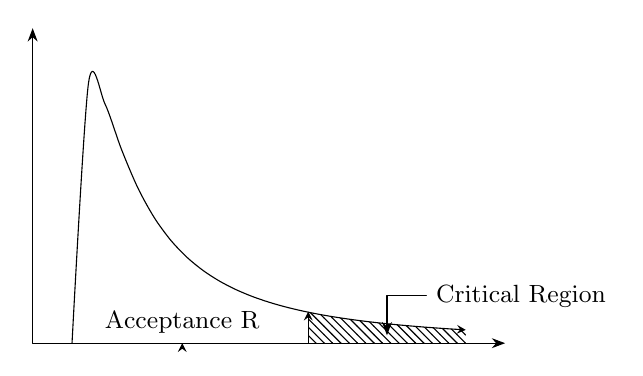
\begin{tikzpicture}[->,>=stealth]
\draw[-Stealth](-0.5,0)--(5.5,0);
\draw[-Stealth](-0.5,0)--(-0.5,4);
\draw[smooth, domain=0:10, scale=0.5,variable=\x]plot(\x,{45*\x/((1 + \x)*(1+\x)*(1+\x))});
\draw(3,0)--(3,0.4);
\path[pattern = north west lines, smooth, domain=6:10, scale=0.5,variable=\x]plot(\x,{45*\x/((1 + \x)*(1+\x)*(1+\x))})--(10,0.17)--(10,0)--(6,0)--(6,0.4)--cycle;
\draw[-Stealth](4.5,0.6)--(4,0.6)--(4,0.1);
\draw(4.5,0.6)node[right]{Critical Region}
(1.4,0)node[above]{Acceptance R};
\end{tikzpicture}
\end{figure}













We accept $H_0$ and $H_1$, since our statistic $F=5.60$ lies in the acceptance  region.\\
$\implies \hspace{0.5cm}$ There is no difference between them.\\\\


\begin{table}[H]
\centering
TWO WAY ANOVA\\
\begin{tabular}{|c|c|c|c|c|}
\hline
Source of Variation & df & SS & MS & F\\
\hline
Between Rows & $r-1=v_1=3$ & $SS_R$ & $\dfrac{SS_R}{r-1}=MS_R$ & $F_R=\dfrac{MS_R}{MSE}$\\
Withing the Columns & $c-1=v_2=2$ & $SS_C$ & $\dfrac{SS_C}{c-1}=MS_C$ & $F_C=\dfrac{MS_C}{MSE}$\\
Errors & $(rc-1)-(c-1)-(r-1)$ & $SSE$ & $\dfrac{SSE}{v_3}=MSE$ &\\
\hline
Total & $rc-1=v_3=6$&&&\\
\hline
\end{tabular}
\end{table}



$$SSE = SST-SS_R-SS_C$$\\

The data below gives the results of variate of the maize against these types of fertilizers.\\

\begin{table}[H]
\centering
fertilizer types
\begin{tabular}{c|ccc|c}
&&variate &&\\
&$v_1$&$v_2$&$v_3$&\\
\hline
$f_1$ & 17 &25&25&69\\
$f_2$ &8 & 10 & 0& 18\\
$f_3$ & 12 & 19 & 11 & 42\\
$f_4$ & 11 &10 &6 & 27\\
\hline
Total &&&&156\\
\end{tabular}
\end{table}

Do the data provide evidence at $\alpha =1\%$ that
\begin{enumerate}
\item[$\longrightarrow$] there is a different between the variates
\item[$\longrightarrow$] there is a difference between the fertilizers\\
\end{enumerate}


\begin{enumerate}
\item Calculate the correction factor \hspace{0.2cm}$\displaystyle{cf=\frac{g^2}{rc}}$
\item Total sum of the squares \hspace{0.2cm}$\displaystyle{SS_T=\sum \sum^k_{ij}x^2_{ij}-cf}$
\item Sum of squares of columns \hspace{0.2cm}$\displaystyle{SS_C=\frac{1}{r}\sum c^2-cf}$
\item Sum of square of rows \hspace{0.2cm}$\displaystyle{SS_R=\frac{1}{c}\sum r^2_i-cf}$
\item $SSE=SS_T-SS_R-SS_C$
\end{enumerate}


$$df: v_1=2, v_2=3, v_3=6$$
\begin{align*}
&(rc-1)-(r-1)-(c-1)\\
&(12-1)-(4-1)-(3-1)\\
&11-3-5\\
&6=v_3
\end{align*}

$$\text{We have that}\hspace{0.3cm} F(\text{Row})=F_{{0.05},3,6}=4.76\hspace{0.3cm} \text{and}\hspace{0.3cm}F(\text{Column})=F_{0.05,2,6}=5.14$$\\
Reject $H_0$\\\\

\textbf{The Least Significant Difference Test (LSD)}
$$\text{The test statistic for the LSD is}\hspace{0.5cm} \text{LSD}=t_{\alpha,v}\hspace{0.1cm}\times \hspace{0.1cm}\sqrt{\frac{1}{n_1}+\frac{1}{n_2}}\hspace{0.3cm},\hspace{0.5cm} v=(n_1+n_2)-2$$ 

We shall use $\widehat{S}=MSE$\\ When $H_0$ is rejected we proceed further for LSD test otherwise not

\begin{table}[H]
\centering
\begin{tabular}{c|cccccc|c}
&\multicolumn{6}{c}{Variates}&\\
&1&2&3&4&5&6&\\
\hline
1&1&3&6&4&3&2&\\
2&1&4&4&8&5&1&\\
3&3&6&7&8&4&3&\\
4&2&3&2&3&2&1&\\
\hline
&7&16&19&23&14&7&81\\
Mean&1.75&4.0&4.75&5.75&3.5&1.75&\\
Total &&&&&&&\\
\end{tabular}
\end{table}
 

\begin{align*}
(1)\hspace{0.4cm} v_1\hspace{0.2cm}Vs\hspace{0.2cm} v_2\hspace{0.2cm}: v_2-v_1=2.25\\\\
(2)\hspace{0.4cm}v_1\hspace{0.2cm}Vs\hspace{0.2cm} v_3\hspace{0.2cm}:1,v_3=3\\\\
(3)\hspace{0.4cm} v_1\hspace{0.2cm}Vs\hspace{0.2cm} v_4 \hspace{0.2cm}: v_1,v_4=4
\end{align*} 


\begin{align*}
t_{0.05,6} & =1.943\\\\
LSD &=1.96\times \sqrt{MSE}\sqrt{\Big(\frac{1}{4}+\frac{1}{4}\Big)}
\end{align*}
 
If LSD $>$ Diff $v_1,v_2$, lies in the C.R then they are significant different.\\\\
$MSE=1.57$, find LSD statistic.\\\\ 

\textbf{Design of Experiments}\\

\begin{table}[H]
\centering
Randomized Design
\begin{tabular}{|cccc|}
\hline
A&B&D&C\\
D&A&C&D\\
C&D&A&B\\
\hline
\end{tabular}
One Way
\end{table}

Randomized Block design\\






\subsection{Completely Randomised Design}
It is the simplest type of design in which the treatments are allocated to the experimental units entirely at random.\\ The design is completely flexible since it allows missing values. Therefore, any number of replicates can be used, replicates may vary from treatment to treatment. The analysis of the experiment under this design is carried out by a one way classification method.

\begin{table}[H]
\centering
\begin{tabular}{c|c|c|c}
$T_1$ & $T_2$ & $T_3$ & $T_4$\\
\hline $X_{11}$ & $X_{12}$ & $X_{13}$ & $X_{14}$\\
$X_{21}$ & $X_{22}$ & $X_{23}$ & $X_{24}$\\
$X_{31}$ & -& $X_{33}$ & $X_{34}$\\
$X_{14}$ &-&-&$X_{44}$\\
\end{tabular}
\end{table}

\textbf{Example}\\
In a comparison of detergents 20, pieces of white cloth were soled with ink. The clothes were washed under controlled conditions with 5 pieces by each of the developer unfortunately 3 pieces went missing in the course of the experiment, whiteness readings are given below:

\begin{table}[H]
\centering
\begin{tabular}{cccc}
A&B&C&D\\ 
77&74&73&76\\
81&58&57&77\\
76&-&69&64\\
69&-&63&-\\
\end{tabular}
\end{table}



Test the hypothesis of no difference between the brands of detergents\\\\ 
cf, SST, SSC, SSE\\\\
ANOVA TABLE?\\\\


\subsection{Randomised Block Design}
In this design the experimental material is divided into groups or Blocks in such a manner that the experimented units within a particular Block are relatively homogeneous. Each Block contains a complete set of treatment. i.e. it constitute a replication of treatments and the treatments are allocated at random to the experimental units within each Block.\\\\

\textbf{Example}\\
The varieties of maize results from RBD are:

\begin{table}[H]
\begin{tabular}{c|c|c|c|c|c|}
$R_1$ & $A_5$ & $C_4$ & $B_5$ & $D_4$ & $E_2$\\
$R_2$ & $B_4$ & $D_3$ & $E_4$ & $C_5$ & $A_6$\\
$R_3$ & $E_3$ & $B_4$ & $C_4$ & $A_3$ & $D_4$\\
\end{tabular}
\end{table}

Test the hypothesis
\begin{enumerate}
\item Between Blocks
\item Between varieties\\
\end{enumerate}

\textbf{Solution}
\begin{enumerate}
\item Set up the hypothesis\\
$H_0:$ There is no difference between blocks\\
$H_1:$ At least two blocks are different\\
\item Set $\alpha=1\%$

\begin{table}[H]
\centering
\begin{tabular}{ccccccc}
$R_1$&5&4&5&4&2&\\
$R_2$&4&3&4&5&6&\\
$R_3$&3&4&4&3&4&\\
\hline &12&11&13&12&12&60\\
\end{tabular}
\end{table}
\end{enumerate}
$$Cf=\frac{g^2}{r\times c}=\frac{3600}{15}=240$$\\

\begin{align*}
\text{SST} &=\sum\sum X^2_{ij}-cf
=
\begin{bmatrix}
5^2+4^2+5^2+4^2+2^2\\ 4^2+3^2+4^2+5^2+6^2\\ 3^2+4^2+4^2+3^2+4^2\\
\end{bmatrix}
-240\\\\
\implies\hspace{0.6cm}\text{SST}&=14\\
\end{align*}

\begin{align*}
\text{SSB} &=\frac{1}{3}\sum c_i^2-cf= \frac{1}{3}(12^2+11^2+13^2+12^2+1^2)-240\\\\ \implies\hspace{0.6cm}\text{SSB} &=0.67\\
\end{align*}

\begin{table}[H]
\centering
\begin{tabular}{ccccc}
A&B&C&D&E\\
5&5&4&4&2\\
6&4&5&3&4\\
3&4&4&4&3\\
\hline 14&13&13&11&9\\
\end{tabular}
\end{table}

\begin{align*}
\text{SS}_T &=\frac{1}{3}\sum \tau_i-cf=\frac{1}{3}\Big[14^2+13^2+13^2+11^2+9^2\Big]-240\\\\ \implies\hspace{0.6cm} \text{SS}_T &=5.3\\
\end{align*}


\begin{align*}
\text{SSE} &=\text{SST}- \text{SSB}- \text{SS}_T\\
&=14-0.67-5.3\\
&=8.03\\
\end{align*}


\begin{table}[H]
\centering
\begin{tabular}{|c|c|c|c|c|c|}
\hline Variation Due to & df & SS & MS & F & $F_{v_1,v_2,\alpha}$\\
\hline &&&&&\\
Blocks & 4 & 0.67 & 0.167 & $F_B=\dfrac{0.167}{1.326}$&\\
Treatments & 4& 5.3 & 1.325& $F_B=\dfrac{1.325}{1.326}$&\\
Error & 6 &8.03 & 1.326&&\\
\hline SST & 14 &&&&\\
\hline
\end{tabular}
\end{table}









\vspace{1cm}
\subsection{Latin Square Design}
In this design we group the experimental units simultaneously in two ways corresponding to two mutually perpendicular direction as rows and columns.\\ Each row and each column is complete replication each treatment appears once in each row and each column.\\ If there are $k$ treatments, experimental area is divided into $k$ rows and $k$ columns results in $k^2$ plots or experimental units.\\ The treatments are then assigned at random to plots.\\\\
\textbf{Example}\\
Analyze the Latin square design by taking $\alpha =0.01$ where $A,B,C,D$ are four types of fertilizer used on the rice crop.\\

\begin{table}[H]
\centering
\begin{tabular}{cccc}
$A_4$&$B_3$&$C_5$&$D_3$\\$B_5$&$A_4$&$D_5$&$C_2$\\$C_4$&$D_2$&$A_3$&$B_3$\\$D_2$&$C_1$&$B_2$&$A_2$\\
\end{tabular}
\end{table}








\pagebreak
\subsection{Practice problems}

\begin{problem}{Sample Questions}
Three systems were compared, each on six occasions:
\begin{table}[H]
\centering
\begin{tabular}{lcccccc}
System A & 55 & 60 & 63 & 56 & 59 & 55\\
System B & 54 & 57 & 53 & 64 & 49 & 62\\
System C & 66 & 52 & 61 & 60 & 57 & 58\\
\end{tabular}
\end{table}
\begin{enumerate}
\item[(a).] Obtain the analysis of variance table, showing all calculations.
\item[(b).] Are the three systems equally effective? Use $\alpha=0.05$.
\item[(c).] Is it necessary to carry out pairwise tests? Give your reasons.
\end{enumerate}
\end{problem}

\begin{solution}
\textbf{(a).} The totals are $T_A=348$, $T_B=339$, $T_C=354$, so the grand total is
$T=1041$ with $n=18$ observations in $k=3$ groups of $n_j=6$.

Start with the correction factor, which appears in every sum of squares:
$$CF=\frac{T^2}{n}=\frac{1041^2}{18}=\frac{1083681}{18}=60204.5.$$
With $\sum\sum x_{ij}^2=60545$,
$$SS_T=\sum\sum x_{ij}^2-CF=60545-60204.5=340.5,$$
$$SS_B=\sum_{j}\frac{T_j^2}{n_j}-CF=\frac{348^2+339^2+354^2}{6}-60204.5=60223.5-60204.5=19.0,$$
$$SS_W=SS_T-SS_B=340.5-19.0=321.5.$$
Note $SS_B$ uses each group's own total $T_j$, not the grand total.

\begin{table}[H]
\centering
\begin{tabular}{lcccc}
Source & $SS$ & df & $MS$ & $F$\\
\hline
Between systems & $19.0$ & $k-1=2$ & $9.50$ & $0.44$\\
Within systems  & $321.5$ & $n-k=15$ & $21.43$ & \\
\hline
Total & $340.5$ & $n-1=17$ & & \\
\end{tabular}
\end{table}
The degrees of freedom add up, $2+15=17$, which is worth checking every time. Note that
$MS_W$ divides $SS_W$ by $n-k=15$, matching its own row.

\textbf{(b).} Testing $H_0:\mu_A=\mu_B=\mu_C$ against the alternative that at least one
differs:
$$F=\frac{MS_B}{MS_W}=\frac{9.50}{21.43}=0.44.$$
The critical value is $F_{2,15,\,0.05}=3.68$, and $0.44$ falls far short of it; the
$P$-value is $0.65$. We fail to reject $H_0$. There is no evidence that the three systems
differ in effectiveness.

Look at why. The group means are $58.0$, $56.5$ and $59.0$ -- a spread of only $2.5$ --
while individual readings within a single system run from $49$ to $66$. The variation
\emph{between} systems is far smaller than the variation \emph{within} them, and $F$ is
precisely the ratio of those two. An $F$ below 1 says the group means are closer together
than one would expect from chance alone.

\textbf{(c).} \textbf{No.} Pairwise tests are what one does \emph{after} a significant $F$,
to find which groups differ. Here $F$ is not significant, so there is nothing to locate:
we have no evidence that any of the systems differ from any other.

Running pairwise tests anyway would be a mistake, and not a harmless one. Three comparisons
each at $5\%$ give a much higher chance than $5\%$ of at least one false positive, which is
the whole reason for testing all groups together with a single $F$ first.
\end{solution}

\section{Linear Regression and Correlation Analysis}


\subsection{Correlation}
The Chi-square test involves the theory of testing whether two attributes of a population are associated with each other. Correlation is concerned with the relation between two variables for a population.\\ We can find out about the relationship between two variables by:
\begin{enumerate}
\item plotting a scatter diagram
\item calculation of the correlation coefficient.\\
\end{enumerate}




\subsection{Scatter diagram}
This involves plotting the variables on the $X-Y$ plane and interpret the diagram, using standard diagrams

% Diagram 20


\begin{figure}[H]
\centering
\begin{tikzpicture}[->,>=stealth]
\draw[-Stealth](-0.5,0)--(3.5,0)node[right]{$x$};
\draw[-Stealth](0,-0.5)--(0,3.5)node[above]{$y$};
\draw(0.5,0.5)node[]{$\ast$}
(1,1)node[]{$\ast$}
(1.5,1.5)node[]{$\ast$}
(2,2)node[]{$\ast$}
(2.5,2.5)node[]{$\ast$}
(3,3)node[]{$\ast$};
\draw(5,2)node[right]{Perfect positive correlation}
(-2,2)node[left]{1};
\end{tikzpicture}
\end{figure}









\begin{figure}[H]
\centering
\begin{tikzpicture}[->,>=stealth]
\draw[-Stealth](-0.5,0)--(3.5,0)node[right]{$x$};
\draw[-Stealth](0,-0.5)--(0,3.5)node[above]{$y$};
\draw(0.5,1)node[]{$\ast$}
(1,1)node[]{$\ast$}
(1.5,1.5)node[]{$\ast$}
(1,0.5)node[]{$\ast$}
(1.5,1)node[]{$\ast$}
(2,1.5)node[]{$\ast$}
(2.5,2)node[]{$\ast$}
(3,2.5)node[]{$\ast$};
\draw(5,2)node[right]{Positive fair correlation}
(-2,2)node[left]{2};
\end{tikzpicture}
\end{figure}







\begin{figure}[H]
\centering
\begin{tikzpicture}[->,>=stealth]
\draw[-Stealth](-0.5,0)--(3.5,0)node[right]{$x$};
\draw[-Stealth](0,-0.5)--(0,3.5)node[above]{$y$};
\draw(0.5,3)node[]{$\ast$}
(1,2.5)node[]{$\ast$}
(1.5,2)node[]{$\ast$}
(2,1.5)node[]{$\ast$}
(2.5,1)node[]{$\ast$}
(3,0.5)node[]{$\ast$};
\draw(5,2)node[right]{Perfect negative correlation}
(-2,2)node[left]{3};
\end{tikzpicture}
\end{figure}







\begin{figure}[H]
\centering
\begin{tikzpicture}[->,>=stealth]
\draw[-Stealth](-0.5,0)--(3.5,0)node[right]{$x$};
\draw[-Stealth](0,-0.5)--(0,3.5)node[above]{$y$};
\draw(3,0.5)node[]{$\ast$}
(2.5,1)node[]{$\ast$}
(2,1.5)node[]{$\ast$}
(1.5,0.5)node[]{$\ast$}
(1,1)node[]{$\ast$}
(1.5,1.5)node[]{$\ast$}
(1,2)node[]{$\ast$}
(0.5,2.5)node[]{$\ast$};
\draw(5,2)node[right]{Negative fair correlation}
(-2,2)node[left]{4};
\end{tikzpicture}
\end{figure}








\begin{figure}[H]
\centering
\begin{tikzpicture}[->,>=stealth]
\draw[-Stealth](-0.5,0)--(3.5,0)node[right]{$x$};
\draw[-Stealth](0,-0.5)--(0,3.5)node[above]{$y$};
\draw(0.5,1)node[]{$\ast$}
(1,1)node[]{$\ast$}
(1.5,1.5)node[]{$\ast$}
(1,0.5)node[]{$\ast$}
(1.5,1)node[]{$\ast$}
(2,1.5)node[]{$\ast$}
(2.5,2)node[]{$\ast$}
(3,2.5)node[]{$\ast$}
(0.5,0.5)node[]{$\ast$}
(1,2)node[]{$\ast$}
(1.5,2)node[]{$\ast$}
(2,1)node[]{$\ast$}
(2,3)node[]{$\ast$}
(2.5,1)node[]{$\ast$}
(2.5,3)node[]{$\ast$}
(3,2)node[]{$\ast$}
(3,1)node[]{$\ast$};
\draw(5,2)node[right]{No correlation}
(-2,2)node[left]{5};
\end{tikzpicture}
\end{figure}





\begin{figure}[H]
\centering
\begin{tikzpicture}[->,>=stealth]
\draw[-Stealth](-0.5,0)--(4.5,0)node[right]{$x$};
\draw[-Stealth](-0.2,-0.5)--(-0.2,3.5)node[above]{$y$};
\draw(0,0)node[above]{$\ast$}
(0.5,1.314)node[]{$\ast$}
(1,2.25)node[]{$\ast$}
(1.5,2.814)node[]{$\ast$}
(2,3)node[]{$\ast$}
(2.5,2.814)node[]{$\ast$}
(3,2.25)node[]{$\ast$}
(3.5,1.314)node[]{$\ast$}
(4,0)node[above]{$\ast$};
\draw(5,2)node[right]{Non linear correlation}
(-2,2)node[left]{6};
\draw(1,0.1)node[]{$\ast$}
(1.25,0.876)node[]{$\ast$}
(1.5,1.5)node[]{$\ast$}
(1.75,1.876)node[]{$\ast$}
(2,2)node[]{$\ast$}
(2.25,1.876)node[]{$\ast$}
(2.5,1.5)node[]{$\ast$}
(2.75,0.876)node[]{$\ast$}
(3,0.1)node[]{$\ast$};
\end{tikzpicture}
\end{figure}







\vspace{0.7cm}

\textbf{Example}\\
Marks obtained in two papers are:
\begin{table}[H]
\centering
\begin{tabular}{c|c}
Paper 1& Paper 2\\
\hline 42&31\\
84&83\\ 50&42\\ 42&60\\ 33&28\\50&63\\ 69&59\\ 81&92\\ 80&73\\ 35&40\\
\end{tabular}
Draw a scatter diagram and interpret your diagram.
\end{table}
In order for you to talk about correlation between two variables, the two variables should be related.\\\\







\subsection{Calculation of Correlation Coefficient}

The correlation coefficient will be in the interval $[-1,1]$.



% Diagram 30



\begin{figure}[H]
\centering
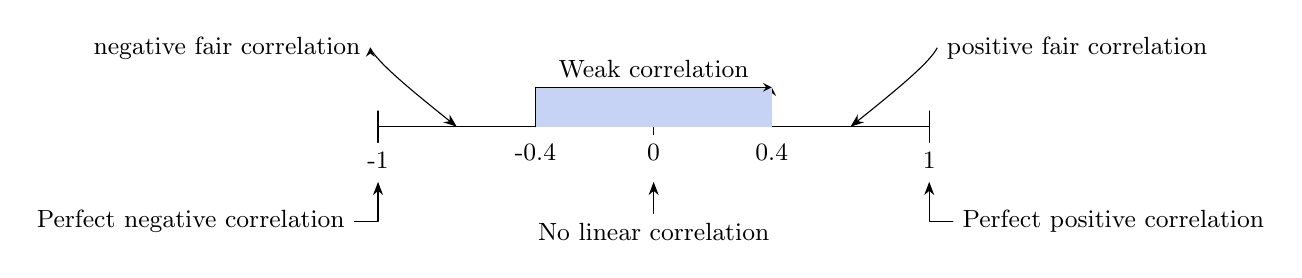
\begin{tikzpicture}[->,>=stealth]
\draw(-3.5,0)--(3.5,0)
(-3.5,-0.2)--(-3.5,0.2)
(3.5,-0.2)--(3.5,0.2)
(0,-0.1)--(0,0.1)
(-1.5,0)--(-1.5,0.5)
(1.5,0)--(1.5,0.5);
\path[fill=blue!25](1.5,0)--(1.5,0.5)--(-1.5,0.5)--(-1.5,0)--cycle;
\draw(-1.5,0.5)--node[above,sloped]{Weak correlation}(1.5,0.5);
\draw(-3.5,-0.2)node[below]{-1}
(3.5,-0.2)node[below]{1}
(0,-0.1)node[below]{0}
(1.5,-0.1)node[below]{0.4}
(-1.5,-0.1)node[below]{-0.4}
(3.8,-1.2)node[right]{Perfect positive correlation}
(-3.8,-1.2)node[left]{Perfect negative correlation}
(0,-1.1)node[below]{No linear correlation}
(3.6,1)node[right]{positive fair correlation}
(-3.6,1)node[left]{negative fair correlation};
\draw[-Stealth](3.8,-1.2)--(3.5,-1.2)--(3.5,-0.7);
\draw[-Stealth](-3.8,-1.2)--(-3.5,-1.2)--(-3.5,-0.7);
\draw[-Stealth](0,-1.1)--(0,-0.7);
\draw[-Stealth](3.6,1)..controls(3.5,0.8)and(3,0.4)..(2.5,0);
\draw[-Stealth](-3.6,1)..controls(-3.5,0.8)and(-3,0.4)..(-2.5,0);
\end{tikzpicture}
\end{figure}









\vspace{0.5cm}


\subsubsection{Pearson Product-Moment Correlation Coefficient}
\begin{align*}
\text{(a).}\hspace{1cm} r&=\frac{\sum(X-\overline{X})(Y-\overline{Y})}{\sqrt{\sum(X-\overline{X})^2}\hspace{0.1cm}.\hspace{0.1cm}\sqrt{\sum(Y-\overline{Y})^2}}\\\\\\
\text{(b).}\hspace{1cm} r&=\frac{n\sum XY-\sum X\sum Y}{\sqrt{n\sum X^2-\Bigg(\sum X\Bigg)^2}\sqrt{n\sum Y^2-\Bigg(\sum Y\Bigg)^2}}\\
\end{align*}

\textbf{Example}
\begin{table}[H]
\begin{tabular}{c|c|c|c|c}
$X$&$Y$&$XY$&$X^2$&$Y^2$\\
\hline 42&31&&&\\
84&83&&&\\50&42&&&\\42&60&&&\\33&28&&&\\50&63&&&\\69&59&&&\\81&92&&&\\50&73&&&\\35&10&&&\\
\end{tabular}
\end{table}






\pagebreak
\subsubsection{Spearman's Rank Correlation Coefficient}
In this case we do not have two continuous variables which are normally distributed but two discrete variables in the form of ranking $$r=1-\frac{6\sum d^2}{n(n^2-1)}$$
If there is an agreement between the two ranks, then $r=1$.\hspace{0.2cm} $d=$ difference between the two ranks.\\





\textbf{Example}\\
Two judges at a competition awarded the following marks to candidates
\begin{table}[H]
\centering
\begin{tabular}{c|ccccccc}
Judge A&5.8&5.5&5.9&4.9&5.9&5.6&5.0\\
\hline Judge B&5.5&5.4&5.8&5.3&5.7&5.7&5.7\\
\end{tabular}
\end{table}


\begin{enumerate}
\item Calculate the Spearmans rank correlation coefficient.
\item Do the judges agree on the order in which they place the candidate.\\
\end{enumerate}




\textbf{Solution}
\begin{table}[H]
\begin{tabular}{cccccc}
Judge A& Rank &Judge B& Rank &$d$& $d^2$\\
\hline 5.8&3&5.5&5&$-2$&4\\
5.5&5&5.4&6&$-1$&1\\ 5.9&3/2&5.8&1&0.5&0.25\\ 4.9&7&5.3&7&0&0\\ 5.9&3/2&5.7&3&$-1.5$&2.25\\ 5.6&4&5.7&3&1&1\\ 5.0&6&5.7&3&3&9\\
\hline &&&&&17.5
\end{tabular}
\end{table}

\begin{align*}
r&=1-\frac{6\sum d^2}{n(n^2-1)}=1-\frac{6\times 17.5}{7(7^2-1)}\\\\ \implies\hspace{0.5cm} r&=0.6875
\end{align*}
There is a positive fair correlation between the judges. So we have that $r_s=0.6875$\\

Now we solve for the second part.\\
Set the hypothesis\\
$H_0$: The  is no correlation between the judges $r_s=0$\\ $H_1:$ There is an association $r_s\neq 0$\\\\ $|r_c|=$ critical value from the table, $n=7$, $|r_c|=0.75$\\ $$r_s=0.6875$$ Since $r_s = 0.6875 < |r_c| = 0.75$, we \textbf{fail to reject} $H_0$ at this level.

Be careful how that is reported. It does \emph{not} show the judges disagree. The observed
$r_s = 0.6875$ is a fairly strong positive association -- it is simply not strong enough,
\emph{with only 7 items}, to rule out chance at this significance level. A test on so few
observations has little power, and the honest conclusion is that there is insufficient
evidence of agreement, not evidence of its absence.\\\\





\subsection{Linear Regression}
When $X$ and $Y$ are linearly related, we can draw a scatter diagram. We can show this relationship between $X$ and $Y$. Our interest is draw a straight line which approximates the points.



% Diagram 31

\begin{figure}[H]
\centering
\begin{tikzpicture}[->,>=stealth]
\draw[-Stealth](-0.5,0)--(4,0);
\draw[-Stealth](0,-0.5)--(0,4);
\draw(0,1)--(3,3);
\draw[-Stealth](1,1.67)--(0.5,2)node[above]{$e_1$};
\draw[-Stealth](2,2.33)--(2.5,2)node[below]{$e_2$};
\draw[-Stealth](2.8,2.87)--(2.8,3.4);
\draw(2.9,3.2)--(3,3.2)node[right]{error};
\end{tikzpicture}
\end{figure}











 
 
 
 
$$Y_i=\alpha +\beta X_i+e_i,\hspace{1cm}\text{and}\hspace{1cm} e_i=Y_i-\alpha -\beta X_i$$
where $\alpha +\beta X_i$ represents the linear relationship between $Y$ and $X_i$ and $e_i$ are a random errors.
\begin{align*}
\beta &=\hspace{0.3cm}\text{coefficient of regression of}\hspace{0.2cm}Y\hspace{0.2cm}\text{and}\hspace{0.2cm}X\\ X&=\hspace{0.3cm}\text{independent variable}\\ Y&=\hspace{0.3cm}\text{dependent variable}\\ \alpha &=\hspace{0.3cm}\text{constant}
\end{align*}
We assume that there's independent of $X_i$ and normally distributed with mean 0 and standard deviation $\sigma_{Y/X}$.\\\\ Our interest is to draw this line by estimating $\alpha$ and $\beta$.\\





\subsubsection{The Method of Least Squares}
The parameters $\alpha$ and $\beta$ are estimated by the method of least squares so called because estimates $\widehat{a}$ and $\widehat{b}$ of $\alpha$ and $\beta$ respectively are chosen so as to minimize $\sum\limits_{i=1}^{n}e_i^2$, the sum of the \emph{squared} errors ($n$ is the number of points on the scatter diagram).
\begin{align*}
Y_i &=\alpha +\beta X_i+e_i\\e_i&=Y_i-\alpha -\beta X_i\\ \sum^n_{i=1} e^2_i &=\sum^n_{i=1}(Y_i-\alpha -\beta X_i)^2
\end{align*}
This expression can be varied by varying $\alpha$ and $\beta$, $\widehat{a}$ and $\widehat{b}$ estimates of $\alpha$ and $\beta$. We choose these $\alpha$ and $\beta$ so that $\sum e^2$ are minimized.\\\\
The appropriate values of $\widehat{a}$ and $\widehat{b}$ are found by partial derivatives. $$Y'=0\hspace{0.5cm}\text{stationary point}$$
$$\sum^n_ie_i^2=\sum^n_i(Y-\alpha -\beta X)^2\hspace{0.2cm}\text{estimate}\hspace{0.2cm}\alpha\hspace{0.2cm}\text{and}\hspace{0.2cm}\beta\hspace{0.2cm}\text{to become}\hspace{0.2cm}\sum^n_ie^2_i=\sum^n_i(Y-\widehat{a}-\widehat{b}X)^2$$ We now take partial derivatives with respect to $\widehat{a}$ and $\widehat{b}$.

\begin{align*}
\frac{\partial}{\partial \widehat{a}}\Bigg(\sum^n_i(Y-\widehat{a}-\widehat{b}X)^2\Bigg)&=0\\\\ 2\Bigg(\sum^n_i(Y-\widehat{a}-\widehat{b}X)\Bigg)(-1) &=0\\\\ -2\sum^n_i(Y-\widehat{a}-\widehat{b}X)&=0 \tag{1}\label{eq:ls1}\\
\end{align*}

\begin{align*}
\frac{\partial}{\partial \widehat{b}}\Bigg(\sum^n_i(Y-\widehat{a}-\widehat{b}X)^2\Bigg)&=0\\\\ -2\sum^n_iX(Y-\widehat{a}-\widehat{b}X)&=0 \tag{2}\label{eq:ls2}\\
\end{align*}

\begin{align*}
\text{Now using equation (1) we have the following}\\
\sum^n_i(Y-\widehat{a}-\widehat{b}X)&=0\\\\ \sum^n_iY-n\widehat{a}-\widehat{b}\sum^n_iX&=0 \tag{3}\label{eq:ls3}\\\\ n\widehat{a}=\sum^n_iY-\widehat{b}\sum^n_iX\hspace{0.5cm}&\implies\hspace{0.5cm} \widehat{a}=\frac{1}{n}\Bigg[\sum^n_iY-\widehat{b}\sum^n_iX\Bigg]\\\\\\ \implies\hspace{0.5cm}\widehat{a}&=\overline{Y}-\widehat{b}\overline{X}\\\\
\end{align*}

\begin{align*}
\text{Also from } \eqref{eq:ls3} \text{, it follows that}\\
\sum^n_1X(Y-\widehat{a}-\widehat{b}X)&=0\\\\ \sum^n_iXY-\widehat{a}\sum^n_iX-\widehat{b}\sum^n_iX^2&=0\\\\ \sum^n_iXY-\sum^n_iX\Bigg[\frac{1}{n}\Bigg(\sum^n_iY-\widehat{b}\sum^n_iX\Bigg)\Bigg]-\widehat{b}\sum^n_iX^2&=0\\\\ \sum^n_iXY-\frac{1}{n}\sum^n_iX\sum^n_iY+\frac{1}{n}\widehat{b}\Bigg(\sum^n_iX\Bigg)^2-\widehat{b}\sum^n_iX^2&=0\\
\end{align*}

\begin{align*}
\widehat{b}\Bigg[\frac{1}{n}\Bigg(\sum^n_iX\Bigg)^2-\sum^n_iX^2\Bigg]&=\frac{1}{n}\sum^n_iX\sum^n_iY-\sum^n_iXY\\\\ \widehat{b}&=\frac{\dfrac{1}{n}\sum\limits^n_iX\sum\limits^n_iY-\sum\limits^n_iXY}{\dfrac{1}{n}\Bigg(\sum\limits^n_iX\Bigg)^2-\sum\limits^n_iX^2}\\\\ \widehat{b}&=\frac{\sum X\sum Y-n\sum XY}{\Bigg(\sum X\Bigg)^2-n\sum X^2}\\\\ \implies\hspace{0.5cm} \widehat{b}=\frac{n\sum XY-\sum X\sum Y}{n\sum X^2-\Bigg(\sum X\Bigg)^2}\\
\end{align*}

Therefore, the relationship between $X$ and $Y$ is given by \hspace{0.1cm}$Y=\widehat{a}+\widehat{b}X\hspace{0.1cm}$ and this is called the Regression line of $Y$ on $X$.

\subsection{Inference for the Regression Line}

Fitting a line is only half the work. Least squares will happily draw a line through points
with no relationship whatever, so the next question is whether the slope we obtained is
real or could plausibly have arisen by chance.

\subsubsection{Partitioning the variation}

Exactly as in the analysis of variance, the total variation in $Y$ splits into a part the
line explains and a part it does not:
$$\underbrace{\sum(Y_i-\overline{Y})^2}_{SS_T}
=\underbrace{\sum(\widehat{Y}_i-\overline{Y})^2}_{SS_R\ \text{(regression)}}
+\underbrace{\sum(Y_i-\widehat{Y}_i)^2}_{SS_E\ \text{(error)}}$$
where $\widehat{Y}_i=\widehat{a}+\widehat{b}X_i$ is the value the line predicts. $SS_E$ is
the sum of squared \textbf{residuals} -- the vertical gaps between the points and the line,
which is precisely the quantity least squares chose $\widehat{a}$ and $\widehat{b}$ to make
as small as possible.

\subsubsection{The coefficient of determination}

\begin{definition_}
The \textbf{coefficient of determination} is
$$R^2=\frac{SS_R}{SS_T}=1-\frac{SS_E}{SS_T},$$
the proportion of the variation in $Y$ that the regression line accounts for.
\end{definition_}

$R^2$ lies between 0 and 1, and in simple linear regression it is exactly the square of the
correlation coefficient, $R^2=r^2$. An $R^2$ of $0.81$ says the line accounts for $81\%$ of
the variation in $Y$; the remaining $19\%$ is unexplained.

Two warnings. A high $R^2$ does not mean the straight-line model is right -- data curving
in a smooth arc can produce a large $R^2$ while a straight line is plainly the wrong shape,
which is why the residuals should always be plotted. And $R^2$ says nothing about
causation: $X$ may predict $Y$ well without influencing it at all.

\subsubsection{The ANOVA table for regression}

\begin{table}[H]
\centering
\begin{tabular}{lcccc}
Source & $SS$ & df & $MS$ & $F$\\
\hline
Regression & $SS_R$ & $1$ & $MS_R=\dfrac{SS_R}{1}$ & $\dfrac{MS_R}{MS_E}$\\[6pt]
Error      & $SS_E$ & $n-2$ & $MS_E=\dfrac{SS_E}{n-2}$ & \\[4pt]
\hline
Total      & $SS_T$ & $n-1$ & & \\
\end{tabular}
\end{table}
The degrees of freedom are worth reading rather than memorising. The total carries $n-1$,
one lost to estimating $\overline{Y}$. The regression carries $1$, because a straight line
has one slope. The error carries $n-2$, since fitting the line used up two estimates,
$\widehat{a}$ and $\widehat{b}$ -- and $1+(n-2)=n-1$, so the table balances.

Under $H_0:\beta=0$ the ratio $F=MS_R/MS_E$ follows an $F$ distribution with $1$ and $n-2$
degrees of freedom. A large $F$ is evidence that the line explains more than chance would.

\subsubsection{Testing and estimating the slope}

The quantity $MS_E$ estimates $\sigma^2$, the variance of the errors about the line, and
its square root $s=\sqrt{MS_E}$ is the standard error of the estimate. The standard error
of the slope is
$$SE(\widehat{b})=\frac{s}{\sqrt{\sum(X_i-\overline{X})^2}}.$$
The denominator carries a useful message: the more spread out the $X$ values, the smaller
the standard error. A line is pinned down more firmly by observations taken over a wide
range of $X$ than by the same number bunched together.

To test $H_0:\beta=0$ against $H_1:\beta\neq 0$, use
$$t=\frac{\widehat{b}-0}{SE(\widehat{b})}, \qquad \text{df}=n-2,$$
and reject when the $P$-value is below $\alpha$. In simple linear regression this $t$-test
and the $F$-test above always agree, because $t^2=F$ -- they are the same test written two
ways.

A confidence interval for the slope is
$$\widehat{b}\pm t_{n-2,\,\alpha/2}\times SE(\widehat{b}),$$
and for the intercept
$$\widehat{a}\pm t_{n-2,\,\alpha/2}\times s\sqrt{\frac{1}{n}+\frac{\overline{X}^2}{\sum(X_i-\overline{X})^2}}.$$
Both use $t$ with $n-2$ degrees of freedom, by the rule from the previous chapter: $\sigma$
is unknown and has been estimated from the data.

The interval for the slope is often more informative than the test. If it excludes zero we
would reject $H_0$ at that level anyway -- but the interval also shows \emph{how large} the
effect might plausibly be, which a $P$-value alone never does.\\\\ The regression line will pass through the point $(\overline{X},\overline{Y})$.



% Diagram 32

\begin{figure}[H]
\centering
\begin{tikzpicture}[->,>=stealth]
\draw[-Stealth](-0.5,0)--(4.5,0);
\draw[-Stealth](0,-0.5)--(0,4);
\draw(0,1)--(4,3.67);
\draw(0,1)node[left]{10}
(0,2.33)node[left]{16}
(2,2.33)node[shape=circle,scale=0.01cm,fill=black]{}
(2,2.2)node[right]{$(\overline{X},\overline{Y})$}
(2,0)node[below]{15}
(3.5,0)node[below]{25};
\draw[dashed](0,2.33)--(2,2.33)--(2,0)
(3.5,0)--(3.5,3.39);
\draw(3.5,3.33)--node[above,sloped]{$Y=\widehat{a} + \widehat{b}X$}(4,3.67);
\end{tikzpicture}
\end{figure}







substituting in the Regression line $\widehat{Y}$- predicted value gives $X=25$.\\\\


\textbf{Example}
\begin{table}[H]
\begin{tabular}{c|cccccccccc}
$X$&0.1&0.2&0.3&0.4&0.5&0.6&0.7&0.8&0.9&1.0\\ $Y$&10.7&11.3&12.0&12.4&13.0&13.7&14.5&15.1&15.6&16\\
\end{tabular}
\end{table}

Find the regression line $Y=\widehat{a}+\widehat{b}X$\\\\


\textbf{Solution}
\begin{table}[H]
\begin{tabular}{|c|c|c|c|c|}
\hline $X$&$Y$&$XY$&$X^2$&$(Y-\widehat{Y})^2$\\
\hline 0.1 &10.7&&&\\
0.2&11.3&&&\\
0.3&12.0&&&\\
0.4&12.4&&&\\
0.5&13.0&&&\\
0.6&13.7&&&\\
0.7&14.5&&&\\
0.8&15.1&&&\\
0.9&15.6&&&\\
1.0&16.0&&&\\
\hline 5.5 &134.4&78.88&3.85&0.11784\\
\hline
\end{tabular}
\end{table}

\begin{align*}
\widehat{b} &=\frac{n\sum XY-\sum X\sum Y}{n\sum X^2-\Bigg(\sum X\Bigg)^2}\hspace{0.5cm}\implies \hspace{0.5cm} \widehat{b}=6.08\\\\
\widehat{a}&=10.1\\
\end{align*}

$\therefore \hspace{0.3cm}$ The regression line of $Y$ on $X$ is $Y=10.1+6.08X$




% Diagram 33

\begin{figure}[H]
\centering
\begin{tikzpicture}[->,>=stealth]
\draw[-Stealth](-0.5,0)--(4,0);
\draw[-Stealth](0,-0.5)--(0,4);
\draw(0,1)--(3,3)node[right]{$Y=10.1 + 6.08X$};
\draw(1,1.67)--(0.5,2)node[above]{$e_1$};
\draw(2,2.33)--(2.5,2)node[below]{$e_2$};
\draw(1,1.1)node[]{$\cdot$}
(1.4,1.5)node[]{$\cdot$}
(1,2.1)node[]{$\cdot$}
(1.4,2.5)node[]{$\cdot$}
(2,1.8)node[]{$\cdot$}
(2.5,2.2)node[]{$\cdot$}
(2,2.5)node[]{$\cdot$}
(2.5,2.9)node[]{$\cdot$}
(2.5,2.8)node[]{$\cdot$}
(1,1.5)node[]{$\cdot$};
\end{tikzpicture}
\end{figure}











 The interpretation of $\widehat{b}=6.08$. This is the expected change in length of the spring with 1 unit increase in weight$(X)$.\\\\ If $X=17$, what is the expected value of $Y$?$$\mu_{Y(X=17)}=10.1+6.08\times 17$$\\
 If $X=18$, what is $P(Y>20)$? $$P(Y>20| X=18)=P\Bigg(\frac{20-18}{\sigma}\Bigg)=1-P(Z<Z_1)$$
 
 The predicted values from the regression line is $\widehat{Y}=\widehat{a}+\widehat{b}X$.\\
 
 If $X=1.2\implies \widehat{Y}=10.1+6.08\times 1.2$\\
 
$\widehat{Y}=17.4$, this is the predicted value for $X=1.2$
 
 \begin{align*}
 \widehat{Y}_i &=\widehat{a}+\widehat{b}X_i\\\\
 \widehat{Y}_1 &=\widehat{a}+\widehat{b}X_1\\
 \widehat{Y}_2 &=\widehat{a}+\widehat{b}X_2\\
 .\\
 .\\
 .\\
 \widehat{Y}_n &=\widehat{a}+\widehat{b}X_n\\
 \end{align*}
$*$ Residuals are deviations of observed and predicted values $$\text{SSE}=\sum_i^ne_i^2=\sum (Y-\widehat{Y})^2$$
Which in turn allows us to estimate $\theta^2$.\\\\
As well as an important statistics referred to as the coefficients of determination
$$R^2=1-\frac{\text{SSE}}{\text{SST}},\hspace{1cm} \text{SST}=\sum^n_i(Y-\widehat{Y})^2$$\\






\subsubsection{Estimating A Value for $\sigma^2_{Y/X}$}
For a value of $X$ the value of $Y$. Predicting by the regression line is given by $\widehat{Y}=\widehat{a}+\widehat{b}X$.\\

The difference between $Y$ and $\widehat{Y}$ is known as a residual, gives the value of $e$ for that point.\\ Each value of $\widehat{Y}-Y$ gives value of $e_i$ from a distribution which is $N(0,\sigma^2_{Y/X})$. The unbiased estimate$\widehat{S}_{Y/X}$ is given by $$\widehat{S}_{Y/X}=\sqrt{\frac{\sum (\widehat{Y}-Y)^2}{n-2}}$$ $n-2$ is the df, $\widehat{a}$, $\widehat{b}$ are calculated from the values of $X$ and $Y$.\\


\textbf{Example}\\
Obtain an estimate of $\sigma^2_{Y/X}$ from the previous example.
$$\widehat{S}_{Y/X}=\sqrt{\frac{0.11784}{8}}\hspace{0.5cm}\implies\hspace{0.5cm} \widehat{S}_{Y/X}=0.121$$
\begin{align*}
P(Y>20|X=18) &=P\Bigg(\frac{20-8}{0.121}\Bigg)=P(16.53)\\\\ &=1-P(Z<16.53)
\end{align*}

\begin{align*}
P(Y>19|X=18) &=P\Bigg(\frac{19-8}{0.121}\Bigg)=P(8.3)\\\\
&=1-P(Z<8.3)=0.99\\
&=0.00099\\
&\approx 0\\
\end{align*}

\subsubsection{Confidence Limit For $\beta$}
How accurate is the estimate $\widehat{b}$ which we have made of $\beta$? Here we want the limit of $\beta$ in terms $\sigma_{Y/X}$ the s.d. of the random error $e_i$.\\ we assume with a normal distribution with mean 0 and s.d. $\sigma_{Y/X}$.
$$E(e)=0\hspace{1cm}\text{and}\hspace{1cm} \text{var}(e)=\sigma^2_{Y/X}$$
We want to calculate the expected value and variance of $\widehat{b}$ in terms of $e_i$


\begin{align*}
\widehat{b} &=\frac{n\sum XY-\sum X\sum Y}{n\sum X^2-\Bigg(\sum X\Bigg)^2}\\\\
\implies &Y=\alpha +\beta X +e\\
\end{align*}
$Y=\beta X+\alpha e$ substitute in $$\widehat{b}=\frac{n\sum X(\beta X+\alpha +e)-\sum X\sum (\beta X+\alpha +e)}{n\sum X^2-\Bigg(\sum X\Bigg)^2}$$
Take the numerator

\begin{align*}
&n\sum X(\beta X+\alpha +e)-\sum X\sum (\beta X+\alpha +e)\\\\ &= n\beta\sum X^2+n\alpha \sum X +n\sum Xe-\Bigg[\beta \Bigg(\sum X\Bigg)^2+\alpha n\sum X +\sum X\sum e\Bigg]\\\\
&=\beta \Bigg[n\sum X^2-\Bigg(\sum X\Bigg)^2\Bigg]+n\sum Xe-\frac{n}{n}\sum X\sum e\\\\ &=\beta \Bigg[n\sum X^2-\Bigg(\sum X\Bigg)^2\Bigg] +n\sum Xe-n\overline{X}\sum e\\\\ &=\beta \Bigg[n\sum X^2-\Bigg(\sum X\Bigg)^2\Bigg]+n\sum (X-\overline{X})e\\
\end{align*}
Dividing the denominator in $\widehat{b}$
\begin{align*}
\widehat{b} &=\frac{\beta \Bigg[n\sum X^2-\Bigg(\sum X\Bigg)^2\Bigg]+n\sum (X-\overline{X})e}{n\sum X^2-\Bigg(\sum X\Bigg)^2}\\\\
&=\beta +\frac{n\sum (X-\overline{X})e}{n\sum X^2-\Bigg(\sum X\Bigg)^2}\\\\
&=\beta +\frac{n\sum (X-\overline{X})e}{n\sum (X-\overline{X})^2}\\\\
\implies\hspace{0.5cm} \widehat{b}&=\beta +\frac{\sum (X-\overline{X})e_i}{\sum (X-\overline{X})^2}
\end{align*}

In this calculation the expected value and variance of $\widehat{b}$.\\\\ The terms in $X_i$ is constant $(X_1-\overline{X}, X_2-\overline{X},........,X_i-\overline{X})$ for each $e_i$ since the value of $X_i$ are pre-determined


\begin{align*}
E(\widehat{b}) &=\beta +\frac{E\Bigg(\sum (X-\overline{X})e_i\Bigg)}{\sum (X-\overline{X})^2}\\\\
&=\beta +\frac{\sum (X-\overline{X})E(e)}{\sum (X-\overline{X})^2}\\\\
& But \hspace{0.5cm} E(e)=0\\
\end{align*}
$\implies\hspace{0.5cm} E(\widehat{b})=\beta\hspace{0.4cm}$ $\widehat{b}$ is an unbiased estimator of $\beta$.\\
\begin{align*}
\text{var}(\widehat{b}) &=\text{var}\Bigg[\frac{\sum (X-\overline{X})e}{\sum (X-\overline{X})^2}\Bigg]\hspace{0.5cm}\implies\hspace{0.5cm}
\text{var}(\widehat{b})=\frac{\sum (X-\overline{X})^2\sum e_i}{\Bigg[\sum (X-\overline{X})^2\Bigg]^2}\\
\text{aX}&=a\text{var}(X)\\\\
\text{var}(X) &=\frac{\sigma^2_{Y/X}}{\sum (X-\overline{X})^2}\\
\end{align*}

Assuming the sampling distribution of $\widehat{b}$ is normal the $95\%$ C.I of $\beta$ is given by 
$$\beta =\widehat{b}\pm \frac{Z_{\alpha/2}\times \sigma_{Y/X}}{\sqrt{\sum (X-\overline{X})^2}}\hspace{0.5cm}\text{If}\hspace{0.3cm}\sigma_{Y/X}^2\hspace{0.3cm} \text{is known}.$$\\
$$\beta =\widehat{b}\pm \frac{t_{n-2,\alpha/2}\times \widehat{S}_{Y/X}}{\sqrt{\sum (X-\overline{X})^2}}\hspace{1cm} \text{if}\hspace{0.3cm}\sigma^2_{Y/X}\hspace{0.3cm}\text{is estimated from}\hspace{0.3cm} \widehat{S}_{Y/X}$$\\

\textbf{Example}\\
To the example above calculate $95\%$ confidence limit for the estimate of $\beta$.
\begin{align*}
\widehat{S}_{Y/X} &=0.121\\
\sum (X-\overline{X}) &=\sum X^2-\frac{\Bigg(\sum X\Bigg)^2}{n}\hspace{1cm}\implies\hspace{0.5cm} \sum (X-\overline{X})=0.825\\
\end{align*}

$$t_{8,0.025}=2.31\hspace{1cm}\text{and}\hspace{1cm} \widehat{b}=6.08$$\\
\begin{align*}
\beta &=6.08\pm \frac{2.31\times 0.121}{\sqrt{0.825}}\hspace{0.5cm} \implies \hspace{0.5cm} \beta =6.08\pm 0.31\\
\end{align*}
$\therefore$ we are $95\%$ confident that the true $\beta$(slope) lies between $$6.08-0.31,\hspace{0.3cm}(5.97)\hspace{0.5cm}\text{and}\hspace{0.5cm} 6.08+0.31,\hspace{0.3cm} (6.39)$$








\pagebreak
\begin{thebibliography}{}
\bibitem{MJDFD}{}
Statistic. Mclave, J.T. and Dietrich, F.H. 1979. Delloen Publishing Company.
\bibitem{WRE}{}
Introduction to statistics. Walpole, R.E. 1984, Macmillan.
\end{thebibliography}
\subsection{Practice problems}

\begin{problem}{Assignment}
Pupils transferring from primary to secondary education are given two verbal reasoning
tests. The scores of twelve pupils, quoted relative to the mean score for each test, are:
\begin{table}[H]
\centering
\begin{tabular}{lcccccccccccc}
Pupil  & A & B & C & D & E & F & G & H & I & J & K & L\\
\hline
Test 1 & $-15$ & $-14$ & $-10$ & $-5$ & $-4$ & $-1$ & 2 & 5 & 10 & 13 & 17 & 20\\
Test 2 & $-10$ & $-7$ & $-4$ & $-6$ & $-1$ & 6 & $-2$ & 5 & 9 & 0 & 10 & 12\\
\end{tabular}
\end{table}
Show that the product-moment correlation coefficient of the test scores is approximately
$0.871$.
\end{problem}

\begin{solution}
Use the computational form, which avoids working out every deviation:
$$r=\frac{n\sum XY-\sum X\sum Y}
{\sqrt{n\sum X^2-\left(\sum X\right)^2}\ \sqrt{n\sum Y^2-\left(\sum Y\right)^2}}.$$
From the table, with $n=12$:
$$\sum X=18,\quad \sum Y=12,\quad \sum XY=837,\quad \sum X^2=1550,\quad \sum Y^2=592.$$
Then
$$n\sum XY-\sum X\sum Y = 12(837)-(18)(12)=10044-216=9828,$$
$$n\sum X^2-\left(\sum X\right)^2=12(1550)-324=18276,$$
$$n\sum Y^2-\left(\sum Y\right)^2=12(592)-144=6960,$$
so
$$r=\frac{9828}{\sqrt{18276}\ \sqrt{6960}}=\frac{9828}{135.19\times 83.43}=0.871,$$
as required.

A word on why the scores being ``quoted relative to the mean'' does not matter. Correlation
is unaffected by adding a constant to either variable, so subtracting each test's mean
beforehand leaves $r$ exactly as it was. It only makes the arithmetic pleasanter.

An $r$ of $0.871$ is a strong positive association: pupils who did well on one test tended
to do well on the other, which is what one would hope of two tests intended to measure the
same thing.
\end{solution}

\begin{problem}{Assignment}
In an experiment the values of two variables $X$ and $Y$ are measured. Ten experiments gave
$$(6,13),\ (12,2),\ (9,12),\ (5,15),\ (2,17),\ (12,5),\ (8,10),\ (3,13),\ (11,12),\ (7,11).$$
\begin{enumerate}
\item[(a).] Find the equation of the regression line of $Y$ on $X$.
\item[(b).] Find $r$ and $R^2$, and say what they mean here.
\item[(c).] Construct the ANOVA table and test whether the slope differs from zero.
\end{enumerate}
\end{problem}

\begin{solution}
\textbf{(a).} With $n=10$,
$$\sum X=75,\quad \sum Y=110,\quad \sum XY=707,\quad \sum X^2=677.$$
$$\widehat{b}=\frac{n\sum XY-\sum X\sum Y}{n\sum X^2-\left(\sum X\right)^2}
=\frac{10(707)-75(110)}{10(677)-75^2}=\frac{7070-8250}{6770-5625}
=\frac{-1180}{1145}=-1.031.$$
$$\widehat{a}=\overline{Y}-\widehat{b}\,\overline{X}=11-(-1.031)(7.5)=18.729.$$
So the regression line is
$$Y=18.729-1.031X.$$
The negative slope says $Y$ falls by about $1.03$ units for each unit increase in $X$. As a
check, the line passes through $(\overline{X},\overline{Y})=(7.5,11)$, as it must.

\textbf{(b).} $r=-0.822$ and $R^2=0.676$.

The sign of $r$ matches the sign of the slope, as it always does. $R^2=0.676$ says the line
accounts for about $68\%$ of the variation in $Y$; the remaining $32\%$ is scatter about
the line that $X$ does not explain.

\textbf{(c).} The fitted values give
$$SS_T=180.0,\qquad SS_R=121.61,\qquad SS_E=58.39,$$
and $SS_R/SS_T=0.676=R^2$, which is a useful arithmetic check.
\begin{table}[H]
\centering
\begin{tabular}{lcccc}
Source & $SS$ & df & $MS$ & $F$\\
\hline
Regression & $121.61$ & $1$ & $121.61$ & $16.66$\\
Error      & $58.39$  & $8$ & $7.30$   & \\
\hline
Total      & $180.00$ & $9$ & & \\
\end{tabular}
\end{table}
Testing $H_0:\beta=0$, the critical value is $F_{1,8,\,0.05}=5.32$ and $16.66$ is well
beyond it. The $P$-value is $0.0035$, so we reject $H_0$: there is strong evidence of a
linear relationship.

The equivalent $t$-test gives the same verdict. With
$s=\sqrt{MS_E}=2.70$ and $\sum(X-\overline{X})^2=114.5$,
$$SE(\widehat{b})=\frac{2.70}{\sqrt{114.5}}=0.2525,
\qquad t=\frac{-1.031}{0.2525}=-4.08$$
on $8$ degrees of freedom, against a critical $2.306$ -- and the same $P$-value of
$0.0035$. Note that
$$t^2=(-4.08)^2=16.66=F,$$
exactly as it must be: in simple linear regression the two tests are one test written two
ways.

A $95\%$ confidence interval for the slope is
$$-1.031\pm 2.306(0.2525)=-1.031\pm 0.582=(-1.613,\ -0.449).$$
It excludes zero, which is the same conclusion again -- but it also says how large the
effect plausibly is, which neither test does on its own.
\end{solution}

\end{document}